% This is the Amherst College LaTeX thesis template.
% See http://web.reed.edu/cis/help/latex.html for help. There are a
% great bunch of help pages there, with notes on
% getting started, bibtex, etc. Go there and read it if you're not
% already familiar with LaTeX.
%
% Any line that starts with a percent symbol is a comment.
% They won't show up in the document, and are useful for notes
% to yourself and explaining commands.
% Commenting also removes a line from the document;
% very handy for troubleshooting problems. -BTS

% As far as I know, this follows the requirements laid out in
% the 2002-2003 Senior Handbook. Ask a librarian to check the
% document before binding. -SN

%%
%% Preamble
%%
% \documentclass{<something>} must begin each LaTeX document
\documentclass[12pt,twoside]{amherstthesis}
% Packages are extensions to the basic LaTeX functions. Whatever you
% want to typeset, there is probably a package out there for it.
% Chemistry (chemtex), screenplays, you name it.
% Check out CTAN to see: http://www.ctan.org/
%%
\usepackage{graphicx,latexsym}
\usepackage{amsmath}
\usepackage{amssymb,amsthm}
\usepackage{longtable,booktabs,setspace}
\usepackage{chemarr} %% Useful for one reaction arrow, useless if you're not a chem major
\usepackage{rotating}

% Modified by CII
\usepackage[hyphens]{url}
\usepackage{hyperref}
\usepackage{lmodern}

% Added by CII (Thanks, Hadley!)
% Use ref for internal links
\renewcommand{\hyperref}[2][???]{\autoref{#1}}
\def\chapterautorefname{Chapter}
\def\sectionautorefname{Section}
\def\subsectionautorefname{Subsection}

\usepackage{caption}
\captionsetup{width=5in}

% \usepackage{times} % other fonts are available like times, bookman, charter, palatino

\title{My Comprehensive Evaluation}
\author{Azka Javaid}
% The month and year that you submit your FINAL draft TO THE LIBRARY (May or December)
\date{May 2017}
\division{Statistics}
\advisor{Nicholas J. Horton}
%If you have two advisors for some reason, you can use the following
%\altadvisor{Your Other Advisor}
%%% Remember to use the correct department!
\department{Mathematics and Statistics}
% if you're writing a thesis in an interdisciplinary major,
% uncomment the line below and change the text as appropriate.
% check the Senior Handbook if unsure.
%\thedivisionof{The Established Interdisciplinary Committee for}
% if you want the approval page to say "Approved for the Committee",
% uncomment the next line
%\approvedforthe{Committee}

% Below added by CII

%%% Copied from knitr
%% maxwidth is the original width if it's less than linewidth
%% otherwise use linewidth (to make sure the graphics do not exceed the margin)
\makeatletter
\def\maxwidth{ %
  \ifdim\Gin@nat@width>\linewidth
    \linewidth
  \else
    \Gin@nat@width
  \fi
}
\makeatother

\renewcommand{\contentsname}{Table of Contents}

\setlength{\parskip}{0pt}

\providecommand{\tightlist}{%
  \setlength{\itemsep}{0pt}\setlength{\parskip}{0pt}}

\Acknowledgements{
\textbar{} I would first like to thank the Amherst College Department of
Mathematics and Statistics and Amherst College Department of Information
Technology (IT) for facilitating this project. I would like to thank
Professor Shu-Min Liao, Professor Pamela B. Matheson and Professor Amy
Wagaman for reviewing the project as well as offering suggestions for
improvement. Additionally I would like to thank Professor Eunice Kim and
Professor Susan Wang for their assistance in the Statistics Program.

This project would not have been possible if it wasn't for Aaron
Coburn's continuous assistance with the Hadoop platform. Additionally, I
would like to thank Andy Anderson and Amherst College Department of IT
for their assistance with the R server.

I would like to thank my classmates from Advanced Data Analysis,
particularly Stephany-Flores Ramos, Jordan Browning and Levi Lee. I
wouldn't have the necessary data wrangling and analytical skills if it
wasn't for the insightful group work. Additionally I would like to thank
Caleb Ki for collaborating on the Advanced Data Analysis group project.

Lastly I would like to thank Professor Nicholas Horton for all his
support with Hadoop, the H2O machine learning platform and for stressing
the importance of statistical analytics, git programming, and
collaborative learning.
}

\Dedication{

}

\Preface{

}

\Abstract{
\textbar{} This study aimed to predict departure delay from 2008 to 2016
against time assessing factors like year, carrier, air time, distance,
week and season. Additionally this work provided an expository review of
modern deep learning techniques like the H2O platform, which was used to
perform modeling techniques like logistic regression and neural networks
in R. Three different models were performed. A simple logistic
regression was used to predict departure delay over 30 minutes against
year, carrier, air time, distance, week and season. A subsequent simple
logistic regression model was built to study influence of weather on
predicting departure delay occurrence over 30 minutes against season,
month, week, weekend, day, hour, distance and air time. Weather
predictors included temperature, dewpoint, humidity, wind direction,
wind speed, wind gust, precipitation, pressure and visibility. Lastly a
deep learning neural network was built to study the influence of
variables like year, month, carrier, distance, hour, week, weekend and
season on predicting departure delay over 90 minutes. Additionally grid,
random search and checkpoint variations of the original models were
developed to facilitate hyperparameter specification. Overall, carrier
type, season, distance and air time were most important at predicting
departure delay occurrence over 30 minutes using logistic regression.
Weather was not very important in predicting departure delay occurrence
over 30 minutes. Hour (5, 6 and 9 am) and carrier status (Hawaiian
Airlines, Northwest, Skywest and US Airlines) were most important at
predicting departure delay over 90 minutes in the deep learning model.
}


%%
%% End Preamble
%%
%

\begin{document}

      \maketitle
  
  \frontmatter % this stuff will be roman-numbered
  \pagestyle{empty} % this removes page numbers from the frontmatter

      \begin{acknowledgements}
      \textbar{} I would first like to thank the Amherst College Department of
      Mathematics and Statistics and Amherst College Department of Information
      Technology (IT) for facilitating this project. I would like to thank
      Professor Shu-Min Liao, Professor Pamela B. Matheson and Professor Amy
      Wagaman for reviewing the project as well as offering suggestions for
      improvement. Additionally I would like to thank Professor Eunice Kim and
      Professor Susan Wang for their assistance in the Statistics Program.
      
      This project would not have been possible if it wasn't for Aaron
      Coburn's continuous assistance with the Hadoop platform. Additionally, I
      would like to thank Andy Anderson and Amherst College Department of IT
      for their assistance with the R server.
      
      I would like to thank my classmates from Advanced Data Analysis,
      particularly Stephany-Flores Ramos, Jordan Browning and Levi Lee. I
      wouldn't have the necessary data wrangling and analytical skills if it
      wasn't for the insightful group work. Additionally I would like to thank
      Caleb Ki for collaborating on the Advanced Data Analysis group project.
      
      Lastly I would like to thank Professor Nicholas Horton for all his
      support with Hadoop, the H2O machine learning platform and for stressing
      the importance of statistical analytics, git programming, and
      collaborative learning.
    \end{acknowledgements}
  
  
  % Add table of abbreviations?

      \hypersetup{linkcolor=black}
    \setcounter{tocdepth}{2}
    \tableofcontents
  
      \listoftables
  
      \listoffigures
  
      \begin{abstract}
      \textbar{} This study aimed to predict departure delay from 2008 to 2016
      against time assessing factors like year, carrier, air time, distance,
      week and season. Additionally this work provided an expository review of
      modern deep learning techniques like the H2O platform, which was used to
      perform modeling techniques like logistic regression and neural networks
      in R. Three different models were performed. A simple logistic
      regression was used to predict departure delay over 30 minutes against
      year, carrier, air time, distance, week and season. A subsequent simple
      logistic regression model was built to study influence of weather on
      predicting departure delay occurrence over 30 minutes against season,
      month, week, weekend, day, hour, distance and air time. Weather
      predictors included temperature, dewpoint, humidity, wind direction,
      wind speed, wind gust, precipitation, pressure and visibility. Lastly a
      deep learning neural network was built to study the influence of
      variables like year, month, carrier, distance, hour, week, weekend and
      season on predicting departure delay over 90 minutes. Additionally grid,
      random search and checkpoint variations of the original models were
      developed to facilitate hyperparameter specification. Overall, carrier
      type, season, distance and air time were most important at predicting
      departure delay occurrence over 30 minutes using logistic regression.
      Weather was not very important in predicting departure delay occurrence
      over 30 minutes. Hour (5, 6 and 9 am) and carrier status (Hawaiian
      Airlines, Northwest, Skywest and US Airlines) were most important at
      predicting departure delay over 90 minutes in the deep learning model.
    \end{abstract}
  
  
  \mainmatter % here the regular arabic numbering starts
  \pagestyle{fancyplain} % turns page numbering back on

  \chapter{Introduction}\label{introduction}
  
  \section{Motivation}\label{motivation}
  
  Airline-related delays (late arrival of 15 minutes) totaled about 20.2
  million minutes in 2015. About 14.3 million minutes of delay was caused
  by weather, congested airports and air traffic system complications.
  Severe weather and security concerns resulted in delays of about 17.5
  million minutes while about 25 million minutes of delay was a result of
  undetermined causes like a previously delayed flight. In total, about 1
  million and 283 thousand hours of delay occurred in 2015 (Levin \&
  Sasso, 2016).
  
  This study strived to assess departure delay from 2008 to 2016. In
  addition, this work aimed to provide an expository review of H2O, the
  Deep Learning and Machine Learning platform, in predicting departure
  delay.
  
  \chapter{Big Data Infrastructure}\label{big-data-infrastructure}
  
  \section{H2O}\label{h2o}
  
  H2O is a big-data machine learning and predictive analytics platform,
  reputable for its fast and scalable deep learning capabilities. Machine
  learning algorithms include supervised and unsupervised learning
  algorithms like neural networks, tree ensembling, generalized linear
  regression models and k-means clustering. H2O provides deep learning
  capabilities through algorithms like perceptrons and feed forward neural
  networks. This platform is built as a Java Virtual Machine (JVM), which
  is an abstract computing environment for running a Java instance
  (Rickert, 2014). H2O clients consequently have a remote connection to
  the data held on the H2O clusters as shown by \autoref{fig:HyarnCluster}
  (Cook, 2016). This contained environment is optimal for performing
  distributed and parallel machine learning computations simultaneously on
  clusters.
  
  \subsection{H2O Installation Process}\label{h2o-installation-process}
  
  H2O installation entails loading Spark 1.6 and H2O version 3.10.06, both
  of which integrate with rsparkling. H2O package can be downloaded from
  (\url{http://h2o-release.s3.amazonaws.com/h2o/rel-turing/6/index.html\#R})\footnote{(``Download
    h2o 3.10.0.6,'' n.d.)}. The rsparkling package can be installed using
  devtools.
  
  Since H2O connection necessitates initialization of a local Spark
  connection, same versions of Spark and Sparkling Water need be
  installed. Desktop version of Spark can be downloaded at
  (\url{http://spark.apache.org/downloads.html})\footnote{(``Download
    apache spark,'' n.d.)}. Desktop version of Sparkling Water can be
  downloaded at
  (\url{http://h2o-release.s3.amazonaws.com/sparkling-water/rel-1.6/8/index.html})\footnote{(``Download
    sparkling water 1.6.8,'' n.d.)}.
  
  \begin{figure}[htbp]
  \centering
  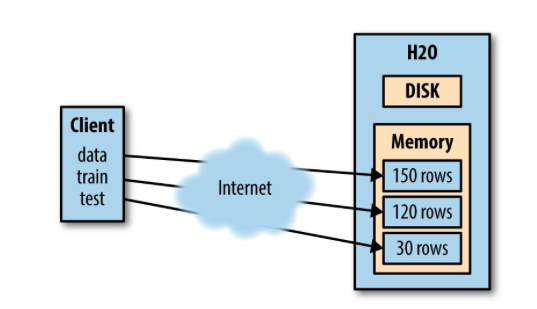
\includegraphics[scale = 0.5,angle = 0]{figure/DataClusters.png}
  \caption[Client and H2O Cluster]{\normalsize{Client and H2O Cluster}}
  \label{fig:HyarnCluster}
  \end{figure}
  
  \section{Apache Spark}\label{apache-spark}
  
  Spark is a big-data platform that provides fast in-memory distributed
  processing. This contrasts with Hadoop, which employs the MapReduce
  processing platform and necessitates data writing to an external disk
  through the Hadoop Distributed File System (HDFS) (Borthakur, n.d.).
  Spark uses the Resilient Distributed Datasets (RDD) data structure,
  which divides the dataset in logical partitions, each of which can be
  processed on separate nodes within clusters. This RDD structure obviates
  the need to write data to an external storage system thus providing
  faster in-memory processing (``Spark programming guide,'' n.d.).
  
  In R, the sparklyr package provides an R interface for Apache Spark.
  This interface facilitates access to Spark's distributed machine
  learning library.
  
  \section{Sparkling Water}\label{sparkling-water}
  
  Sparkling Water combines the machine learning capabilities of H2O with
  the in-memory distributed, fast computation of the Spark platform.
  Tachyon, which is an in-memory distributed file system, facilitates
  exchange of data between Spark and H2O (Ambati, n.d.). The rsparkling
  package in R provides access to H2O's machine learning routines within
  the Spark platform accessible over R. Spark data frames can be converted
  to H2O frames for machine learning and deep learning algorithm
  implementation.
  
  \section{RSparkling}\label{rsparkling}
  
  The rsparkling package facilitates data transfer between Spark and H2O
  dataframes. Rsparkling also allows access to Sparkling Water's machine
  learning algorithms (``Sparkling water (h20) machine learning,'' n.d.).
  
  \section{Hadoop YARN}\label{hadoop-yarn}
  
  Apache Hadoop YARN includes separate resource management and job
  scheduling infrastructures in collective resource manager and individual
  node manager through a master-slave hierarchy (as shown by
  \autoref{fig:Hyarn}(``Spark programming guide,'' n.d.)). The
  per-application based application masters negotiate resources with the
  resource manager and execute and monitor tasks in collaboration with
  node managers. The resource managers additionally contain a scheduler
  that arranges jobs based on resource requirements. Individual node
  managers are responsible for launching application containers and
  examining resource use (like memory and disk consumption). Updates are
  then reported back to the resource manager. Per-node application master
  negotiate resource containers with scheduler (Murthy, 2012).
  
  \begin{figure}[htbp]
  \centering
  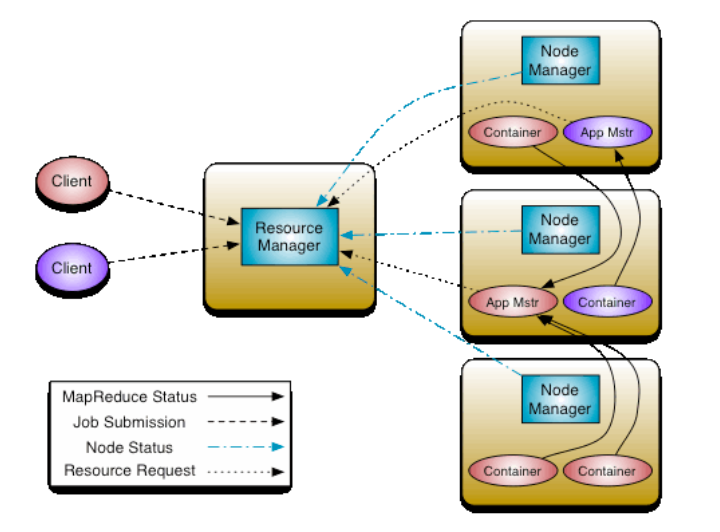
\includegraphics[scale = 0.5,angle = 0]{figure/yarn.png}
  \caption[Hadoop YARN architecture]{\normalsize{Hadoop YARN architecture}}
  \label{fig:Hyarn}
  \end{figure}
  
  \section{Additional Resources}\label{additional-resources}
  
  \begin{itemize}
  \item
    H2O Installation guide -
    \url{http://h2o-release.s3.amazonaws.com/h2o/rel-turing/6/index.html\#R}
  \item
    H2O Documentation -
    \url{http://h2o-release.s3.amazonaws.com/h2o/rel-lambert/5/docs-website/index.html}
  \item
    Sparkling Water Installation -
    \url{http://www.h2o.ai/download/sparkling-water/}
  \item
    Sparkling Water Overview - \url{http://spark.rstudio.com/h2o.html}
  \item
    Sparklyr Overview and Installation - \url{http://spark.rstudio.com}
  \end{itemize}
  
  \chapter{Shiny Application}\label{shiny-application}
  
  \section{Introduction}\label{introduction-1}
  
  Flights dataset from The United States Department of Transportation
  Bureau of Transportation Statistics was used for Shiny visualization.
  The dataset (from 2008-2016) was set up in YARN-client cluster in the
  Hadoop server. Initially it contained variables like year, month and day
  of the trip, departure delay, arrival delay, carrier, tail number,
  distance covered, flight number, flight origin, destination and
  scheduled flight time. Additional predictors were created to assess
  departure delay. These variables included day of week, season, weekend
  status, and hour of flight delay.
  
  Since only flights with departure delay greater than 90 minutes were
  used for deep learning analysis, a table was constructed to show the
  percentage of flights with departure delay greater than 90 minutes from
  the orignal dataset (created as a combination of data from individual
  years). A random sample of 200,000 observations with departure delay
  greater than 90 minutes was selected from the observations shown in
  table 3.1.
  
  \begin{longtable}[]{@{}rrrr@{}}
  \caption{Percentage of observations with \textgreater{}90 minutes
  delay}\tabularnewline
  \toprule
  Year & TotalFlights & NumberDelayed & PercentDelayed\tabularnewline
  \midrule
  \endfirsthead
  \toprule
  Year & TotalFlights & NumberDelayed & PercentDelayed\tabularnewline
  \midrule
  \endhead
  2008 & 7009726 & 235476 & 3.36\tabularnewline
  2009 & 6450285 & 176710 & 2.74\tabularnewline
  2010 & 6450117 & 176460 & 2.74\tabularnewline
  2011 & 6085281 & 176120 & 2.89\tabularnewline
  2012 & 6096761 & 166902 & 2.74\tabularnewline
  2013 & 6369482 & 208306 & 3.27\tabularnewline
  2014 & 5819811 & 198631 & 3.41\tabularnewline
  2015 & 5819079 & 188433 & 3.24\tabularnewline
  2016 & 2289826 & 63429 & 2.77\tabularnewline
  \bottomrule
  \end{longtable}
  
  \section{Web Scraping}\label{web-scraping}
  
  Since carrier, departure airport and destination airport information was
  provided as two and three letter code names, following the guidelines
  set by the International Air Transport Association (IATA), additional
  data was scraped from web to include the origin and destination airport
  information as well as the carrier and state names. This data was then
  merged with the flights dataset. Data scraping was performed using the
  rvest package and the SelectorGadget tool, a Chrome extension that
  allows for easy CSS webpage selection (see Appendix 2 for complete
  scraping code).
  
  \section{Shiny App}\label{shiny-app}
  
  A shiny application was created for initial exploratory analysis.
  Graphical, tabular and weather analysis was performed. Images from the
  shiny app are shown below each commentary. The app itself can be
  accessed at \url{https://aj17.shinyapps.io/flightsapp/}.
  
  \subsection{Tabular Analysis}\label{tabular-analysis}
  
  The tabular analysis displayed the mean departure delay for all flights
  for the specified origin and destination states. In addition, the panel
  showed departure delays for all flights for the user selected origin and
  destination airports.
  
  \subsection{Path Analysis}\label{path-analysis}
  
  Path analysis tab shows flights from a specified origin and destination
  state for a chosen year for all flights with departure delay greater
  than 90 minutes. Point width represents the extent of departure delay in
  minutes. The application was set up so that a point click reveals
  information about the orgin and destination state and airports along
  with the average departure delay for that trip in minutes. An example of
  paths from California to New York is shown by \texttt{ref("shiny90")}
  
  \begin{figure}[htbp]
  \centering
  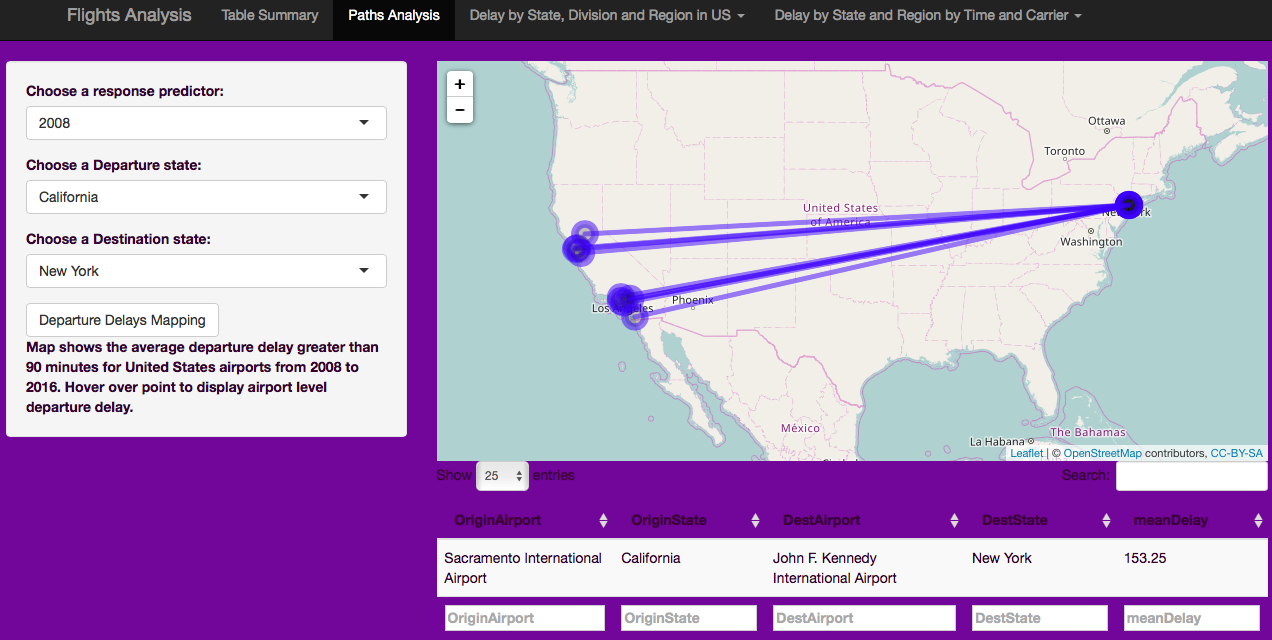
\includegraphics[scale = 0.35,angle = 0]{figure/PathsAnalysis2.png}
  \caption[Paths Analysis from California to New York in 2008]{\normalsize{Paths Analysis from California to New York in 2008}}
  \label{fig:shiny90}
  \end{figure}
  
  \subsection{Departure Delay Analysis}\label{departure-delay-analysis}
  
  \subsubsection{Delay by State, Region and
  Division}\label{delay-by-state-region-and-division}
  
  Departure delay analysis was graphically performed at state, region and
  division level. The first tab shows departure delay by airports for the
  selected state and the aggregated delays for the selected state over all
  airports from 2008 to 2016. In addition, departure delay by four regions
  (Midwest, Northeast, South and West) was analyzed. Each region is
  further analyzed by division. Midwest region is analyzed by East North
  Central and West North Central divisions. Northeast is analyzed by
  Middle Atlantic and New England divisions. South by East South Central,
  West South Central and South Atlantic divisions. Lastly Pacific and
  Mountain divisions are analyzed for Western United States. For each
  region analysis, state-wide trends in the divisions for that region as
  well as aggregate departure delay over 2008 to 2016 are shown. An output
  example for Northeast is shown by \autoref{fig:shiny7}.
  
  \begin{figure}[htbp]
  \centering
  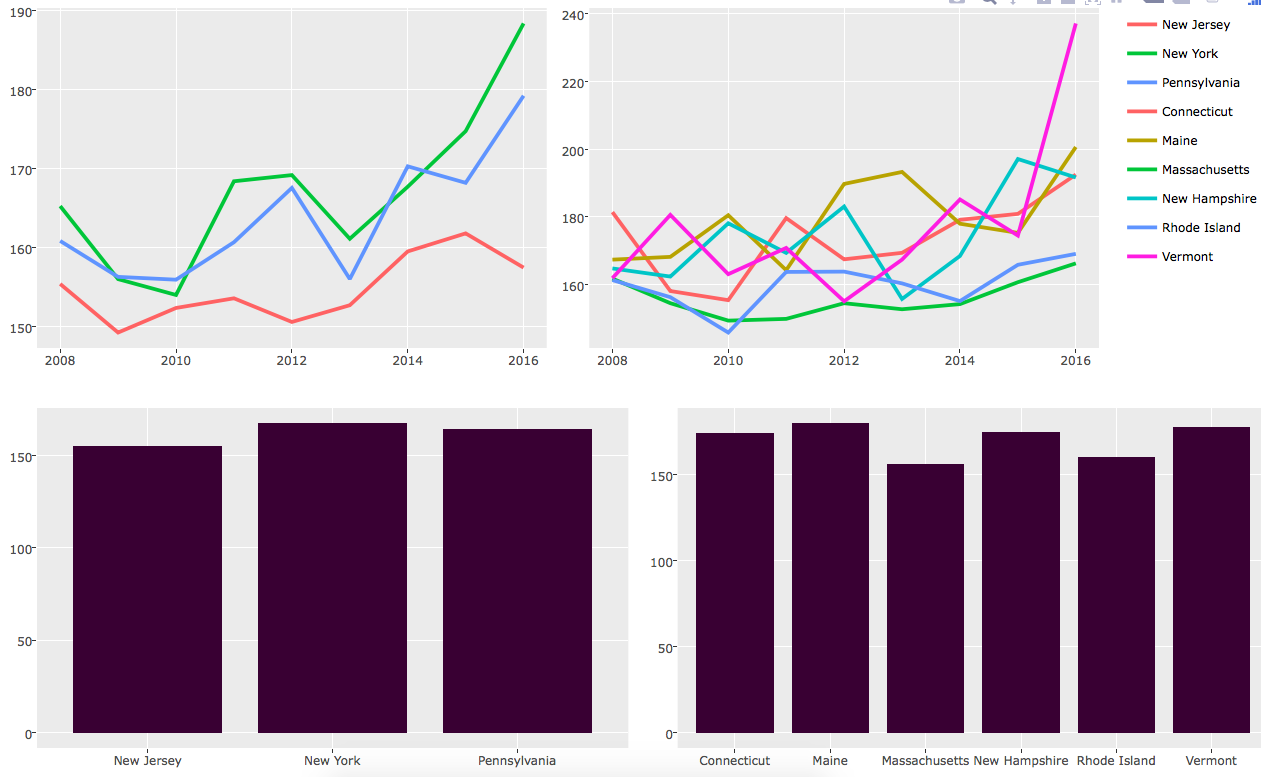
\includegraphics[scale = 0.4,angle = 0]{figure/Northeast1.png}
  \caption[Departure Delay by Region and Division]{\normalsize{Departure Delay by Region and Division}}
  \label{fig:shiny7}
  \end{figure}
  
  \subsubsection{Delay by State and Region over Time and
  Carrier}\label{delay-by-state-and-region-over-time-and-carrier}
  
  In addition to departure delay analysis at the state, region and
  division level, delay was analyzed by variables including hour, day of
  week, weekend status, month, season and carrier type. Analysis was
  performed at regional (Midwest, notheast, south, west) and state levels.
  A general trend pointed towards high delays in South and Midwest in late
  night/early morning hours. Northeast region appears to have the highest
  delays over the week with the highest delays occurring on Sunday and
  weekends. Departure delays in Northeast (June, July, August) are high in
  the summer season while delays are high in spring (April, May) in South.
  In regards to carrier analysis, Hawaiian Airlines experiences the
  highest delay in Northeast and West region. Example below shows delay by
  weekday for Midwest, Northeast, South and Western regions as depicted by
  \autoref{fig:shiny77}.
  
  \begin{figure}[htbp]
  \centering
  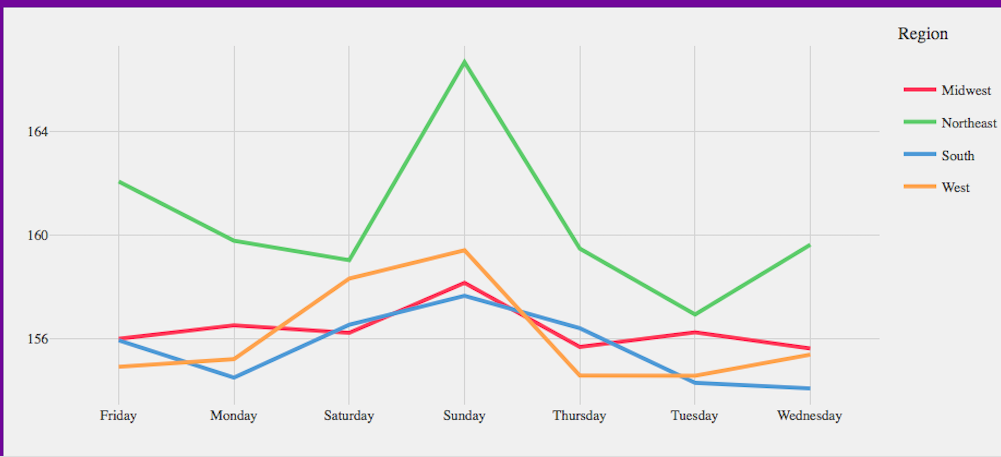
\includegraphics[scale = 0.4,angle = 0]{figure/DelayWeekday.png}
  \caption[Departure Delay by Region over Weekday]{\normalsize{Departure Delay by Region over Weekday}}
  \label{fig:shiny77}
  \end{figure}
  
  \clearpage
  
  \subsection{Aggregate United States Departure
  Delays}\label{aggregate-united-states-departure-delays}
  
  The last shiny panel displays the mean departure delay by airport from
  2008 to 2016 in the United States for all flights with departure delay
  greater than 90 minutes. The dataset for this panel was created by
  filtering all flights with delay greater than 90 minutes for every year
  from 2008 to 2016, resulting in 1,590,467 observations. This data was
  then aggregated by origin and destination airports and year to produce a
  smaller dataset containing 39,277 observations. Hovering over the points
  displays the state, airport and the average departure delay for that
  airport.
  
  \clearpage
  
  \chapter{Logistic Regression}\label{logistic-regression}
  
  \section{Introduction}\label{introduction-2}
  
  H2O platform was used to construct a logistic regressions model to
  predict departure delay occurrence over 30 minutes for flights data from
  The United States Department of Transportation Bureau of Transportation
  Statistics from 2008 to 2016. Cutoff of 30 minutes provided adequate
  sample size for flights that either experienced or did not experience
  departure delay over 30 minutes. Analysis was performed on a random
  sample of 200,000 observations since this dataset of this size could
  easily be transferred to the Spark environment. Occurrence of delay over
  30 minutes was assessed against year, carrier, air time, distance, week
  and season as predictors. Initially, hour, month and weekend status
  predictors were also used to estimate departure delay incidence though
  they appeared to have no importance and therefore were not used in
  subsequent analyses.
  
  \section{H2O Connection}\label{h2o-connection}
  
  H2O connection was established to local host using h2o.init() using
  default 1GB of memory. Additional cluster memory can be allocated with
  max\_mem\_size specification. Since this project was performed using the
  Apache Spark platform, spark connection was established with the YARN
  Hadoop cluster.
  
  \begin{Shaded}
  \begin{Highlighting}[]
  \KeywordTok{library}\NormalTok{(sparklyr)}
  \KeywordTok{library}\NormalTok{(rsparkling)}
  \KeywordTok{library}\NormalTok{(dplyr)}
  \KeywordTok{options}\NormalTok{(}\DataTypeTok{rsparkling.sparklingwater.version =} \StringTok{"1.6.8"}\NormalTok{)}
  
  \CommentTok{#Initialize a cluster (without Hadoop connection)}
  \KeywordTok{h2o.init}\NormalTok{()}
  
  \CommentTok{#Connect to YARN through shell}
  \KeywordTok{kinit}\NormalTok{()}
  \NormalTok{klist  }
  
  \CommentTok{#Connect to Apache Spark Hadoop in markdown }
  \NormalTok{sc <-}\StringTok{ }\KeywordTok{spark_connect}\NormalTok{(}\DataTypeTok{master =} \StringTok{"yarn-client"}\NormalTok{)}
  \end{Highlighting}
  \end{Shaded}
  
  \section{Spark Data Integration}\label{spark-data-integration}
  
  Once spark connection was estabished, flights dataset from 2008-2016 was
  allocated by copying flights data from 2008 to 2016 from Hadoop to the
  Spark environment (see Appendix 2 for full details on the dataset
  creation).
  
  \begin{Shaded}
  \begin{Highlighting}[]
  \CommentTok{#If connection is established to Hadoop:}
  \KeywordTok{load}\NormalTok{(}\StringTok{"HadoopLogMod.Rda"}\NormalTok{)}
  \KeywordTok{set.seed}\NormalTok{(}\DecValTok{134}\NormalTok{)}
  \NormalTok{sample <-}\StringTok{ }\NormalTok{FullDatLog[}\KeywordTok{sample}\NormalTok{(}\KeywordTok{nrow}\NormalTok{(FullDatLog), }
                                \DecValTok{200000}\NormalTok{, }\DataTypeTok{replace =} \OtherTok{FALSE}\NormalTok{, }
                                \DataTypeTok{prob =} \OtherTok{NULL}\NormalTok{),]}
  \NormalTok{LogDataMod <-}\StringTok{ }\KeywordTok{copy_to}\NormalTok{(sc, sample, }\StringTok{"LogData"}\NormalTok{, }
                        \DataTypeTok{overwrite =} \OtherTok{TRUE}\NormalTok{)}
  
  \CommentTok{#If no connection established to Hadoop: }
  \CommentTok{#Read from local file}
  \NormalTok{FlightsDat =}\StringTok{ }\KeywordTok{h2o.importFile}\NormalTok{(localH2O, }\DataTypeTok{path =} \NormalTok{prosFlights)}
  \CommentTok{#Convert to h2o data frame}
  \NormalTok{FlightsDat <-}\StringTok{ }\KeywordTok{as.h2o}\NormalTok{(sample)}
  \end{Highlighting}
  \end{Shaded}
  
  \section{Data Partitioning}\label{data-partitioning}
  
  After data was copied, it was partitioned into test and training sets.
  An approximate 75/25 partition was used where the training dataset was
  allocated about 75\% of the data (149,789 observations) and test set was
  allocated about 25\% (50,211 observations).
  
  \begin{Shaded}
  \begin{Highlighting}[]
  \CommentTok{#Partitioning data frame in Spark }
  \NormalTok{partitions <-}\StringTok{ }\NormalTok{LogDataMod %>%}
  \StringTok{  }\KeywordTok{sdf_partition}\NormalTok{(}\DataTypeTok{training =} \FloatTok{0.75}\NormalTok{, }\DataTypeTok{test =} \FloatTok{0.25}\NormalTok{, }\DataTypeTok{seed =} \DecValTok{1099}\NormalTok{)}
  
  \CommentTok{#Partitioning data locally within the H2O platform}
  \NormalTok{splits <-}\StringTok{ }\KeywordTok{h2o.splitFrame}\NormalTok{(LogDataMod, }\KeywordTok{c}\NormalTok{(}\FloatTok{0.75}\NormalTok{,}\FloatTok{0.25}\NormalTok{), }\DataTypeTok{seed=}\DecValTok{1099}\NormalTok{)}
  \end{Highlighting}
  \end{Shaded}
  
  \section{Checking Conditions}\label{checking-conditions}
  
  Logistic regression necessitated satisfaction of linearity, randomness
  and independence conditions. Since the response (dep\_delayIn) was a
  binary variable indicating the incidence of departure delay of 30
  minutes, linearity was assumed. Randomness and independence may not
  necessarily be valid assumptions since late flight typically results in
  subsequent delays. Analysis of the randomness and independence
  assumption will require tracking flight schedules from 2008 to 2016.
  Future studies could further assess this assumption. This study
  proceeded with caution and therefore findings from this paper need be
  examined conservatively.
  
  \section{Modeling}\label{modeling}
  
  Once data was partitioned, logistic regression model was specified as
  shown. The h2o.glm function was used to specify a binomial family
  function. Additional arguments in the h2o.glm function included nfolds
  (specifies the number of folds for cross validation), alpha (0-1 numeric
  that specifies the elastic-net mixing parameter, set to ensure
  regularization and consequently prevent overfitting), lambda (specifies
  a non-negative shrinkage parameter) and lambda\_search (logical
  indicating whether or not search is conducted over the specified lambda
  space). H2O models can additionally be stopped early with specification
  of metrics like misclassification error, rsquared and mean squared
  error. Every model has an associated model id which can be referenced
  for future model iterations. In the model below, a 5-fold cross
  validation was performed with alpha level of 0.1. As mentioned, the
  logistic model shown below attempted to predict departure delay
  occurrence by variables like year, carrier, air time, distance, week and
  season.
  
  \begin{Shaded}
  \begin{Highlighting}[]
  \NormalTok{myX =}\StringTok{ }\KeywordTok{setdiff}\NormalTok{(}\KeywordTok{colnames}\NormalTok{(training), }\KeywordTok{c}\NormalTok{(}\StringTok{"dep_delayIn"}\NormalTok{, }
                                      \StringTok{"orig_id"}\NormalTok{, }\StringTok{"hour"}\NormalTok{, }
                                      \StringTok{"month"}\NormalTok{, }\StringTok{"weekend"}\NormalTok{))}
   
  \NormalTok{regmod <-}\StringTok{ }\KeywordTok{h2o.glm}\NormalTok{(}\DataTypeTok{y =} \StringTok{"dep_delayIn"}\NormalTok{, }\DataTypeTok{x =} \NormalTok{myX, }
                    \DataTypeTok{training_frame =} \NormalTok{training, }\DataTypeTok{family =} \StringTok{"binomial"}\NormalTok{,}
          \DataTypeTok{alpha =} \FloatTok{0.1}\NormalTok{, }\DataTypeTok{lambda_search =} \OtherTok{FALSE}\NormalTok{, }\DataTypeTok{nfolds =} \DecValTok{5}\NormalTok{)}
  \end{Highlighting}
  \end{Shaded}
  
  \section{Model Assessment}\label{model-assessment}
  
  Model performance was assessed with the h2o.performance function, which
  provides access to evaluation metrics like MSE, RMSE, LogLoss, AUC and
  \(R^{2}\). The \(R^{2}\) for this model was 0.0088 and the AUC was 0.586
  as shown by \autoref{fig:Hyarn20}. The \(R^{2}\) value indicated that
  only about 0.9\% of the variation in departure delay was accounted for
  by predictors year, carrier, air time, distance, week and season. In
  addition to the h2o.performance function, h2o.auc and
  h2o.confusionMatrix (see \autoref{fig:Hyarn26}) were used to retrieve
  the analogous parameters. The AUC curve was visualized as shown by
  figure \autoref{fig:Hyarn48} with the plot(h2o.performance) command. The
  curve with arched midway visually shows area convergence of about 50\%.
  
  \begin{Shaded}
  \begin{Highlighting}[]
  \KeywordTok{h2o.performance}\NormalTok{(regmod) }
  \KeywordTok{h2o.auc}\NormalTok{(regmod) }
  \KeywordTok{h2o.confusionMatrix}\NormalTok{(regmod) }
  \NormalTok{accuracy <-}\StringTok{ }\NormalTok{(mat$No[}\DecValTok{1}\NormalTok{]+mat$Yes[}\DecValTok{2}\NormalTok{])/(mat$No[}\DecValTok{1}\NormalTok{]+}
  \StringTok{                                      }\NormalTok{mat$No[}\DecValTok{2}\NormalTok{]+mat$Yes[}\DecValTok{1}\NormalTok{]+}
  \StringTok{                                      }\NormalTok{mat$Yes[}\DecValTok{2}\NormalTok{]) }
  \KeywordTok{plot}\NormalTok{(}\KeywordTok{h2o.performance}\NormalTok{(regmod)) }\CommentTok{#plot the auc curve }
  \end{Highlighting}
  \end{Shaded}
  
  \begin{figure}[htbp]
  \centering
  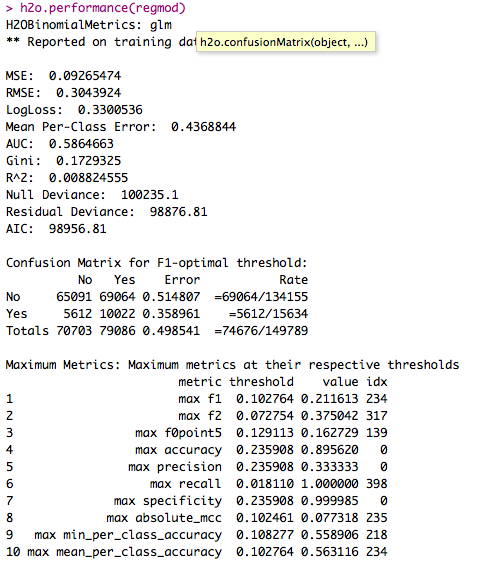
\includegraphics[scale = 0.7,angle = 0]{figure/PerformanceLogMod.png}
  \caption[Model Performance]{\normalsize{Model Performance}}
  \label{fig:Hyarn20}
  \end{figure}
  
  \begin{figure}[htbp]
  \centering
  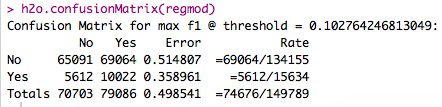
\includegraphics[scale = 0.8,angle = 0]{figure/confMatLog.png}
  \caption[Confusion Matrix]{\normalsize{Confusion Matrix}}
  \label{fig:Hyarn26}
  \end{figure}
  
  \begin{figure}[htbp]
  \centering
  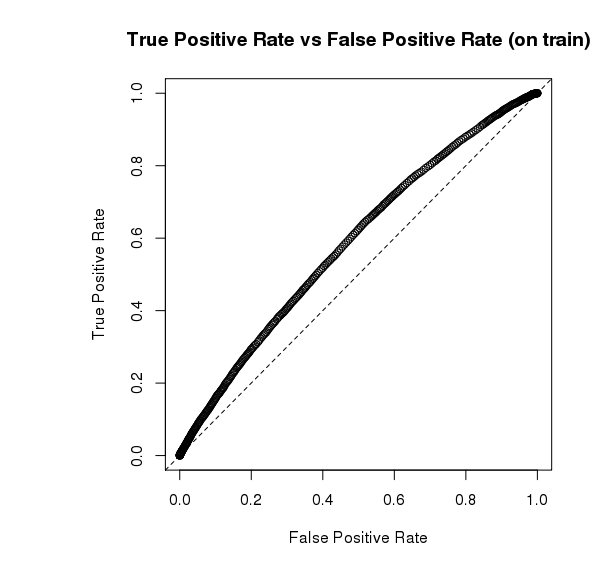
\includegraphics[scale = 0.8,angle = 0]{figure/ROCCurveLog.png}
  \caption[AUC Curve]{\normalsize{AUC Curve}}
  \label{fig:Hyarn48}
  \end{figure}
  
  \clearpage
  
  As the variable importance plot in \autoref{fig:Hyarn34} shows, carrier
  type was the most important predictor of departure delay over 30
  minutes. Hawaiian Airlines (HA) was most negatively associated with
  departure delay. Carrier Spirit (NK) was positively associated with
  departure delay. Additionally, carriers Alaska (AS), US Air (US) were
  negative predictors of departure delay while carriers JetBlue (B6) and
  Atlantic Southeast Airlines were positive predictors of departure delay
  greater than 30 minutes. Season fall was a negative predictor of
  departure delay while summer was a positive predictor of departure delay
  over 30 minutes. Air time was a positive indicator of departure delay
  over 30 minutes while distance was a negative predictor of departure
  delay over 30 minutes.
  
  \begin{Shaded}
  \begin{Highlighting}[]
  \KeywordTok{h2o.varimp}\NormalTok{(regmod) }\CommentTok{#compute variable importance}
  \KeywordTok{h2o.varimp_plot}\NormalTok{(regmod) }\CommentTok{#plot variable importance}
  \end{Highlighting}
  \end{Shaded}
  
  \begin{figure}[htbp]
  \centering
  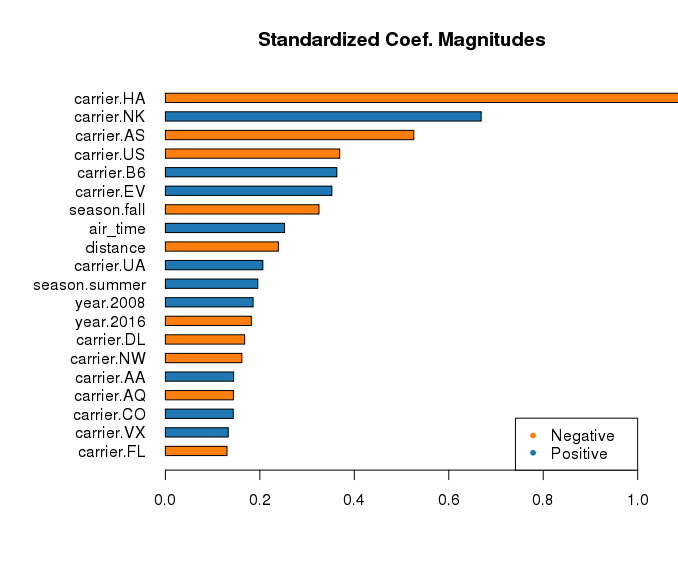
\includegraphics[scale = 1,angle = 0]{figure/LogVarImp.png}
  \caption[Variable Importance for Logistic Regression Analysis]{\normalsize{Variable Importance for Logistic Regression Analysis}}
  \label{fig:Hyarn34}
  \end{figure}
  
  \clearpage
  
  \section{Making Predictions}\label{making-predictions}
  
  After model assessments were analyzed, predictions were performed on the
  test set. The accuracy of the test set was calculated and compared with
  the accuracy of the cross-validated training set. Accuracy of the test
  set of 0.5077 compared with the accuracy of the training data of 0.5015.
  While the accuracy of the training and test data was not very high, the
  error rates for both data were comparable thereby reducing overfitting
  likelihood.
  
  \begin{Shaded}
  \begin{Highlighting}[]
  \NormalTok{pred <-}\StringTok{ }\KeywordTok{h2o.performance}\NormalTok{(}\DataTypeTok{object =} \NormalTok{regmod, }\DataTypeTok{newdata =} \NormalTok{test) }
  \KeywordTok{mean}\NormalTok{(pred$predict==test$dep_delayIn) }\CommentTok{#accuracy of test set }
  \end{Highlighting}
  \end{Shaded}
  
  \section{Conclusion}\label{conclusion}
  
  This chapter discussed concepts like setting up a H2O Yarn connection,
  dataset partitioning, linear regression modeling and model assessments.
  Overall carrier type appeared to be most important in predicting
  departure delay over 30 minutes. Predictors like season, air time and
  distance were important. It must be noted though since the \(R^{2}\)
  value was only about 0.0088 meaning about 0.9\% of the variation in
  departure delay was covered by the chosen predictors, the model does not
  have strong practical significance or predictive ability given an
  accuracy of about 50\%.
  
  \chapter{Logistic Regression and
  Weather}\label{logistic-regression-and-weather}
  
  \section{Introduction}\label{introduction-3}
  
  The H2O platform was used to perform logistic regression to predict
  departure delay over 30 minutes using weather data from the nycflights13
  package for LaGuardia, John F. Kennedy and Newark Liberty International
  airports in 2013. Analysis was performed on data containing 48,126
  observations. Occurrence of delay over 30 minutes was assessed against
  season, month, week, weekend, day, hour, distance and air time. Weather
  predictors included temperature, dewpoint, humidity, wind direction,
  wind speed, wind gust, precipitation, pressure and visibility.
  
  \section{Data Partitioning}\label{data-partitioning-1}
  
  Data from the nycflights13 package was copied in the Spark environment
  followed by a 75/25 partitioning. The training data contained about
  36,153 observations and the test set contained 11,973 observations.
  
  \begin{Shaded}
  \begin{Highlighting}[]
  \KeywordTok{library}\NormalTok{(sparklyr)}
  \KeywordTok{library}\NormalTok{(rsparkling)}
  \KeywordTok{library}\NormalTok{(dplyr)}
  \KeywordTok{options}\NormalTok{(}\DataTypeTok{rsparkling.sparklingwater.version =} \StringTok{"1.6.8"}\NormalTok{)}
  \NormalTok{sc <-}\StringTok{ }\KeywordTok{spark_connect}\NormalTok{(}\DataTypeTok{master =} \StringTok{"yarn-client"}\NormalTok{)}
  \KeywordTok{load}\NormalTok{(}\StringTok{"flights_weather2.Rda"}\NormalTok{)}
  
  \NormalTok{partitions <-}\StringTok{ }\NormalTok{LogDataMod %>%}
  \StringTok{  }\KeywordTok{sdf_partition}\NormalTok{(}\DataTypeTok{training =} \FloatTok{0.75}\NormalTok{, }\DataTypeTok{test =} \FloatTok{0.25}\NormalTok{, }\DataTypeTok{seed =} \DecValTok{1099}\NormalTok{)}
  
  \CommentTok{#Partitioning data locally within the H2O platform}
  \NormalTok{splits <-}\StringTok{ }\KeywordTok{h2o.splitFrame}\NormalTok{(LogDataMod, }\KeywordTok{c}\NormalTok{(}\FloatTok{0.75}\NormalTok{,}\FloatTok{0.25}\NormalTok{), }\DataTypeTok{seed=}\DecValTok{1099}\NormalTok{)}
  \end{Highlighting}
  \end{Shaded}
  
  \section{Checking Conditions}\label{checking-conditions-1}
  
  Linearity was assumed given the binary nature of the response variable
  assessing whether or not departure delay over 30 minutes occurred.
  Randomness and independence may not necessarily be valid assumptions
  since a late flight typically results in subsequent delays. The study
  proceeded with caution.
  
  \section{Modeling}\label{modeling-1}
  
  Logistic model was used to predict departure delay against weather
  predictors like season, month, week, weekend, day, hour, distance, air
  time, temprature, dewpoint, humidity, wind direction, wind speed, wind
  gust, precipitation, pressure and visibility. Same parameters as
  specified in logistic model in the previous chapter were used (alpha =
  0.1, lambda\_search = FALSE and 5-folds cross-validation).
  
  \begin{Shaded}
  \begin{Highlighting}[]
  \NormalTok{myX =}\StringTok{ }\KeywordTok{setdiff}\NormalTok{(}\KeywordTok{colnames}\NormalTok{(training), }\KeywordTok{c}\NormalTok{(}\StringTok{"dep_delayIn"}\NormalTok{)) }\CommentTok{#set difference}
   
  \NormalTok{regmodWeather <-}\StringTok{ }\KeywordTok{h2o.glm}\NormalTok{(}\DataTypeTok{y =} \StringTok{"dep_delayIn"}\NormalTok{, }\DataTypeTok{x =} \NormalTok{myX, }
                    \DataTypeTok{training_frame =} \NormalTok{training, }\DataTypeTok{family =} \StringTok{"binomial"}\NormalTok{,}
          \DataTypeTok{alpha =} \FloatTok{0.1}\NormalTok{, }\DataTypeTok{lambda_search =} \OtherTok{FALSE}\NormalTok{, }\DataTypeTok{nfolds =} \DecValTok{5}\NormalTok{)}
  \end{Highlighting}
  \end{Shaded}
  
  \section{Model Assessment}\label{model-assessment-1}
  
  Model performance was assessed with the h2o.performance function.
  \(R^{2}\) for this model was 0.109 and the AUC was 0.704 as shown by
  \autoref{fig:weath1}. The \(R^{2}\) value indicated that about 11\% of
  the variation in the departure delay variable was captured by season,
  month, week, weekend, day, hour, distance, air time, temprature,
  dewpoint, humidity, wind direction, wind speed, wind gust,
  precipitation, pressure and visibility. In addition to the
  h2o.performance function, h2o.confusionMatrix (see \autoref{fig:weath2})
  was used to retrieve the confusion matrix. The AUC curve was visualized
  as shown by figure \autoref{fig:weath3}.
  
  \begin{Shaded}
  \begin{Highlighting}[]
  \KeywordTok{h2o.performance}\NormalTok{(regmodWeather) }
  \KeywordTok{h2o.auc}\NormalTok{(regmodWeather) }
  \KeywordTok{h2o.confusionMatrix}\NormalTok{(regmod) }
  \NormalTok{accuracy <-}\StringTok{ }\NormalTok{(mat$No[}\DecValTok{1}\NormalTok{]+mat$Yes[}\DecValTok{2}\NormalTok{])/(mat$No[}\DecValTok{1}\NormalTok{]+}
  \StringTok{                                      }\NormalTok{mat$No[}\DecValTok{2}\NormalTok{]+mat$Yes[}\DecValTok{1}\NormalTok{]+}
  \StringTok{                                      }\NormalTok{mat$Yes[}\DecValTok{2}\NormalTok{]) }
  \KeywordTok{plot}\NormalTok{(}\KeywordTok{h2o.performance}\NormalTok{(regmodWeather)) }\CommentTok{#plot the auc curve }
  \end{Highlighting}
  \end{Shaded}
  
  \begin{figure}[htbp]
  \centering
  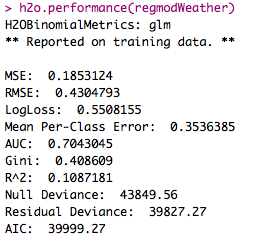
\includegraphics[scale = 0.7,angle = 0]{figure/regmodPerformWeather.png}
  \caption[Model Performance]{\normalsize{Model Performance}}
  \label{fig:weath1}
  \end{figure}
  
  \begin{figure}[htbp]
  \centering
  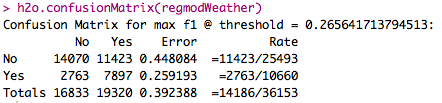
\includegraphics[scale = 0.8,angle = 0]{figure/regModWeather2.png}
  \caption[Confusion Matrix]{\normalsize{Confusion Matrix}}
  \label{fig:weath2}
  \end{figure}
  
  \begin{figure}[htbp]
  \centering
  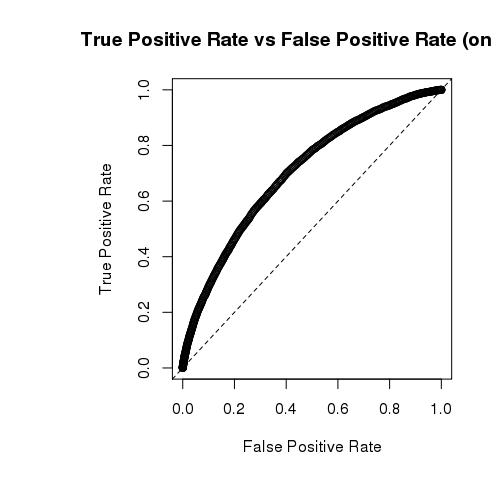
\includegraphics[scale = 0.8,angle = 0]{figure/LogWeatherROC.png}
  \caption[AUC Curve]{\normalsize{AUC Curve}}
  \label{fig:weath3}
  \end{figure}
  
  \clearpage
  
  As shown in the variable importance plot in \autoref{fig:weath4}, air
  time and distance were important in predicting departure delay over 30
  minutes. While air time was a negative predictor of departure delay,
  distance was a positive indicator of departure delay over 30 minutes.
  Hours 5, 6 and 7 am were negative predictors of departure delay over 30
  minutes. In comparison, hours 6, 7 and 8 pm were positive predictors of
  departure delay over 30 minutes. Intuitively, this result suggested that
  there is a higher likelihood of experiencing departure delay greater
  than 30 minutes in evening than in early morning hours. Weather was not
  very important since humidity was the only important positive predictor
  (ranked 36th out of 40) of departure delay greater than 30 minutes.
  
  \begin{Shaded}
  \begin{Highlighting}[]
  \KeywordTok{h2o.varimp}\NormalTok{(regmodWeather) }\CommentTok{#compute variable importance}
  \KeywordTok{h2o.varimp_plot}\NormalTok{(regmodWeather) }\CommentTok{#plot variable importance}
  \end{Highlighting}
  \end{Shaded}
  
  \begin{figure}[htbp]
  \centering
  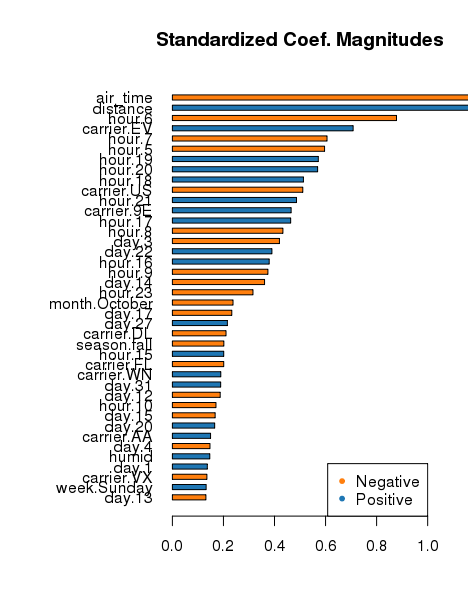
\includegraphics[scale = 1,angle = 0]{figure/top40Weather.png}
  \caption[Variable Importance for Weather Logistic Regression]{\normalsize{Variable Importance for Weather Logistic Regression}}
  \label{fig:weath4}
  \end{figure}
  
  \clearpage
  
  \section{Making Predictions}\label{making-predictions-1}
  
  After model assessments were analyzed, predictions were performed on the
  test set. The accuracy of the test set was calculated and compared with
  the accuracy of the cross-validated training set. In this case, accuracy
  of the test set of 0.612 compared with the accuracy of the training set
  of 0.608. Since the error rates were similar, overfitting occurrence was
  reduced.
  
  \begin{Shaded}
  \begin{Highlighting}[]
  \NormalTok{pred <-}\StringTok{ }\KeywordTok{h2o.performance}\NormalTok{(}\DataTypeTok{object =} \NormalTok{regmodWeather, }\DataTypeTok{newdata =} \NormalTok{test) }
  \KeywordTok{mean}\NormalTok{(pred$predict==test$dep_delayIn) }\CommentTok{#accuracy of test set }
  \end{Highlighting}
  \end{Shaded}
  
  \section{Conclusion}\label{conclusion-1}
  
  This chapter assessed the effects of weather on departure delay aiming
  to examine the role of weather metrics like temperature, dewpoint,
  humidity, wind direction, wind speed, wind gust, precipitation, pressure
  and visibility on departure delay while controlling for predictors like
  distance and air time. Overall air time and distance were the most
  important predictors. Hour was also important in predicting departure
  delay over 30 minutes. Predictors assessing weather were not important.
  While the model including weather produced a \(R^{2}\) of 0.10 (higher
  than the \(R^{2}\) for logistic model without weather), \(R^{2}\) of
  0.10 nonetheless indicates that most of the variation in departure delay
  is unaccounted for by the explanatory predictors including weather.
  
  \chapter{Deep Learning}\label{deep-learning}
  
  \section{Introduction}\label{introduction-4}
  
  \subsection{Machine Learning and Deep
  Learning}\label{machine-learning-and-deep-learning}
  
  Machine learning is the process of insight extraction from natural data
  like speech, text and images to develop pattern-recognition systems,
  transcribe speech in natural language processing (NLP), develop
  reinforcement learning models, identify data anomalies and create
  user-targetted recommendation systems. Conventional machine learning
  models are limited in their capacity to build intricate models from raw
  data of large scale (dataset like ImageNet containing about 15 million
  images) (Krizhevsky, Sutskever, \& Hinton, n.d.). Representation
  learning methods like deep learning provide the ability to automatically
  extract data insights for detection or classification. Deep learning
  provides multiple levels of representation through its non-linear module
  functionality, which transforms data from initial level to a more
  complex state (LeCun, Bengio, \& Hinton, 2015). Learned process' ability
  to automatically extract insights using general-purpose learning process
  provides agility and dynamicity to deep learning models.
  
  Machine Learning is conventionally divided in supervised and
  unsupervised learning. Supervised learning requires labeled data and is
  used to perform operations like image processing. Supervised learning
  includes algorithms like regression, neural networks, random forest and
  support vector machines. Unsupervised learning, on the other hand,
  attempts to locate patterns in unlabeled data and includes algorithms
  like k-nearest neighbor, which use distance metrics to find natural data
  groupings.
  
  This section explores the application of neural networks in a Deep
  Learning context, which describe layered neural networks. Deep learning
  is used in fields like science, advertisement, and business for high
  dimensional natural data processing including image and speech
  recognition, drug molecule activity prediction and natural language
  processing procedures like sentiment analysis and topic classification.
  
  \section{H2O Deep Learning}\label{h2o-deep-learning}
  
  H2O Deep Learning follows the multi-layer, feedforward neural network
  model (Reddy, n.d.). In the feedforward neural network model, the inputs
  are weighted, combined and transmitted as output signal by the connected
  neuron. Function f shown in \autoref{fig:Hyarn6} shows a nonlinear
  activation function where the bias accounts for the activation threshold
  (Candel, Lanford, LeDell, Parmar, \& Arora, 2015). A nonlinear
  activation function ensures that the linearly input hidden layers
  experience variation. Otherwise the output will simply be a linear
  combination of the hidden layers making hidden layers irrelevant.
  Examples of activation functions include sigmoid and rectified linear
  unit (ReLU). The multi-layer platform consists of layers of
  interconnected neurons, which are composed of nonlinear layers
  culminating in a regression or classification layer (Candel et al.,
  2015). An example of a multi-layer neural network is shown in
  \autoref{fig:Hyarn7} (Candel et al., 2015).
  
  \begin{figure}[htbp]
  \centering
  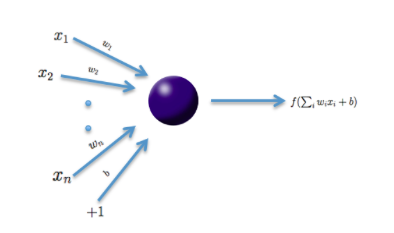
\includegraphics[scale = 0.6,angle = 0]{figure/neuralNet.png}
  \caption[Neural Network]{\normalsize{Neural Network}}
  \label{fig:Hyarn6}
  \end{figure}
  
  \begin{figure}[htbp]
  \centering
  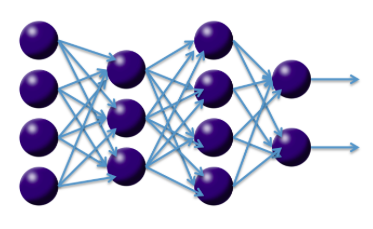
\includegraphics[scale = 0.5,angle = 0]{figure/neuralHid.png}
  \caption[Hidden Layers]{\normalsize{Hidden Layers}}
  \label{fig:Hyarn7}
  \end{figure}
  
  Overall H2O's deep learning functionalities include specification of
  regularization options, learning rate, annealing, hyperparameter
  optimization and model selection through grid and random search.
  Additionally H2O facilitates automatic categorical and numerical data
  processing along with automatic missing data imputation.
  
  H2O deep learning platform was used to predict departure delay over 90
  minutes. The response variable was a continuous predictor capturing
  extent of departure delay in minutes. While the dataset used to perform
  logistic regression contained a binary response indicating the
  occurrence of departure delay over 30 minutes, deep learning was
  performed with a stringent criteria of 90 minutes since a larger delay
  is more likely to incur financial expenses. The explanatory predictors
  of interest for the deep learning model included year, month, carrier,
  distance, hour, week, weekend and season.
  
  \clearpage 
  
  \section{Data Partitioning}\label{data-partitioning-2}
  
  Before data preparation and model building, connection was established
  to the YARN client. Following connection, data sample of 200,000 was
  obtained, which provided easy transferability to the Spark environment.
  Since hyperparameter optimization was performed in the deep learning
  algorithm, a validation data set in addition to a test set was used for
  additional verification. Data was split 60/20/20 consisting of 60\%
  training, 20\% validation and 20\% test set.
  
  \begin{Shaded}
  \begin{Highlighting}[]
  \KeywordTok{options}\NormalTok{(}\DataTypeTok{rsparkling.sparklingwater.version =} \StringTok{"1.6.8"}\NormalTok{)}
  \NormalTok{sc <-}\StringTok{ }\KeywordTok{spark_connect}\NormalTok{(}\DataTypeTok{master =} \StringTok{"yarn-client"}\NormalTok{)}
  
  \KeywordTok{set.seed}\NormalTok{(}\DecValTok{12}\NormalTok{)}
  \NormalTok{thousand <-}\StringTok{ }\NormalTok{FullDat[}\KeywordTok{sample}\NormalTok{(}\KeywordTok{nrow}\NormalTok{(FullDat), }\DecValTok{200000}\NormalTok{, }\DataTypeTok{replace =} \OtherTok{FALSE}\NormalTok{, }
                             \DataTypeTok{prob =} \OtherTok{NULL}\NormalTok{),]}
  \NormalTok{mtcars_tbl <-}\StringTok{ }\KeywordTok{copy_to}\NormalTok{(sc, thousand, }\StringTok{"mtcars"}\NormalTok{, }\DataTypeTok{overwrite =} \OtherTok{TRUE}\NormalTok{) }
  
  \NormalTok{partitions <-}\StringTok{ }\NormalTok{mtcars_tbl %>%}
  \StringTok{  }\KeywordTok{sdf_partition}\NormalTok{(}\DataTypeTok{training =} \FloatTok{0.6}\NormalTok{, }\DataTypeTok{validation =} \FloatTok{0.20}\NormalTok{, }\DataTypeTok{test =} \FloatTok{0.20}\NormalTok{, }
                  \DataTypeTok{seed =} \DecValTok{1099}\NormalTok{)}
  \end{Highlighting}
  \end{Shaded}
  
  \clearpage 
  
  \section{Model Building}\label{model-building}
  
  Following data partitioning, h2o.deeplearning function was used to
  predict departure delay over 90 minutes as a function of year, month,
  carrier, distance, hour, week, weekend and season. The h2o.deeplearning
  function includes specification of the explanatory (x) and response
  predictors (y). In addition, h2o.deeplearning paramaters include
  activation function specification (Tanh, TanhWithDropout, Rectifier,
  RectifierWithDropout, Maxout, MaxoutWithDropout, see
  \autoref{fig:Hyarn77} (Candel et al., 2015)), training and
  validation\_frame delineation along with fine-tuning parameters like
  maximum model iterations, regularization parameters like l1 and l2,
  non-negative shrinkage parameter lambda and cross validation parameter
  (nfolds) specifying number of folds and model iterations, respectively.
  A random seed can also be specified though this is only reproducible
  with algorithms running on a single thread. Additionally
  h2o.deeplearning model provides the ability to stop the model learning
  early if no apparent changes in the loss function are observed.
  
  \begin{figure}[htbp]
  \centering
  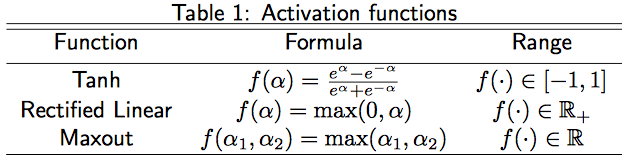
\includegraphics[scale = 0.5,angle = 0]{figure/activationFunc.png}
  \caption[Activation Function]{\normalsize{Activation Function}}
  \label{fig:Hyarn77}
  \end{figure}
  
  A simple model shown below was constructed to predict departure delay
  over 90 minutes as a function of the explantory variables. An epoch of
  one, indicating a single data iteration, was specified. In addition,
  5-fold cross validation was used. Tanh activation layer was used since
  it is more adept at exponentially rising functions and consequently
  appropriate for regularization.
  
  \begin{Shaded}
  \begin{Highlighting}[]
  \NormalTok{myX =}\StringTok{ }\KeywordTok{setdiff}\NormalTok{(}\KeywordTok{colnames}\NormalTok{(training), (}\StringTok{"dep_delay"}\NormalTok{))}
  \NormalTok{deepmod <-}\StringTok{ }\KeywordTok{h2o.deeplearning}\NormalTok{(}
    \DataTypeTok{y=}\StringTok{"dep_delay"}\NormalTok{,}
    \DataTypeTok{x=}\NormalTok{myX,}
    \DataTypeTok{activation=}\StringTok{"Tanh"}\NormalTok{,  }
    \DataTypeTok{training_frame=}\NormalTok{training, }
    \DataTypeTok{validation_frame=}\NormalTok{validation,}
    \DataTypeTok{epochs=}\DecValTok{1}\NormalTok{,}
    \DataTypeTok{variable_importances=}\NormalTok{T,   }
    \DataTypeTok{nfolds =} \DecValTok{5}\NormalTok{,}
    \DataTypeTok{keep_cross_validation_predictions=}\NormalTok{T}
  \NormalTok{)}
  \end{Highlighting}
  \end{Shaded}
  
  A variable importance plot was used to view the most important
  predictors produced by deepmod. In this case, a plot of the top 20
  predictors was produced. As \autoref{fig:Hyarn81} shows, hour and
  carrier type were most important at predicting departure delay greater
  than 90 minutes. Hours 6 am and 5 am along with 9 pm were important at
  predicting departure delay greater than 90 minutes. Additionally
  carriers Northwest (NW), US Air (US) and Frontier (F9) were important at
  predicting departure delay greater than 90 minutes. Besides hour and
  carrier type, flights in April were important at predicting departure
  delay greater than 90 minutes.
  
  \begin{Shaded}
  \begin{Highlighting}[]
  \KeywordTok{h2o.varimp_plot}\NormalTok{(deepmod, }\DataTypeTok{num_of_features =} \DecValTok{20}\NormalTok{)}
  \end{Highlighting}
  \end{Shaded}
  
  \begin{figure}[htbp]
  \centering
  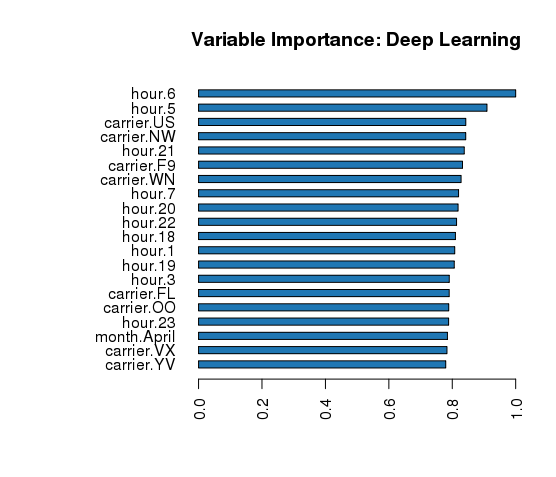
\includegraphics[scale = 1,angle = 0]{figure/VarImpDeep.png}
  \caption[Deep Learning Variable Importance]{\normalsize{Deep Learning Variable Importance}}
  \label{fig:Hyarn81}
  \end{figure}
  
  \clearpage 
  
  \section{Model Assessment}\label{model-assessment-2}
  
  Since the response variable was a continuous indicator of departure
  delay, mean squared error (MSE) was used as an error metric to assess
  the performance of the deep learning model.
  
  As shown by \autoref{fig:Hyarn9}, the MSE on training data was 6522.2
  while MSE on validation data was 6918.5. In comparison, MSE on test data
  was 7010.6. Since MSE for the validation and test data was higher than
  MSE on training data, this was an indication of good fit. Overfitting
  did not appear to be an issue since the difference between the MSE of
  the training, validation and test set was not especially high. The model
  results however need to be considered cautiously due to the high MSE.
  
  \begin{Shaded}
  \begin{Highlighting}[]
  \NormalTok{deepmod@parameters  }
  \KeywordTok{h2o.performance}\NormalTok{(deepmod, }\DataTypeTok{train =} \OtherTok{TRUE}\NormalTok{)  }
  \KeywordTok{h2o.performance}\NormalTok{(deepmod, }\DataTypeTok{valid =} \OtherTok{TRUE}\NormalTok{)  }
  \KeywordTok{h2o.performance}\NormalTok{(deepmod, }\DataTypeTok{newdata =} \NormalTok{test)}
  \end{Highlighting}
  \end{Shaded}
  
  \begin{figure}[htbp]
  \centering
  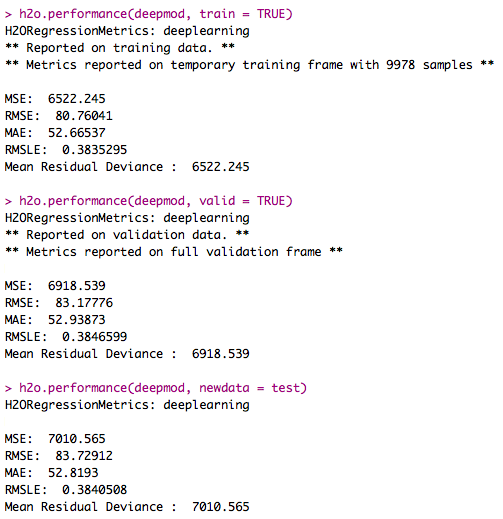
\includegraphics[scale = 0.7,angle = 0]{figure/deepModml.png}
  \caption[Deep Learning Model Performance]{\normalsize{Deep Learning Model Performance}}
  \label{fig:Hyarn9}
  \end{figure}
  
  \clearpage 
  
  \section{Saving Model}\label{saving-model}
  
  Once the model was constructed, it was saved using the h2o.saveModel
  command as shown below with the path specification.
  
  \begin{Shaded}
  \begin{Highlighting}[]
  \NormalTok{DeepModel <-}\StringTok{ }\KeywordTok{h2o.saveModel}\NormalTok{(m1, }\DataTypeTok{path =} \StringTok{"/home/ajavaid17"}\NormalTok{, }\DataTypeTok{force =} \OtherTok{FALSE}\NormalTok{) }
  \end{Highlighting}
  \end{Shaded}
  
  Model can be loaded with the h2o.loadModel command with the specified
  path as an argument.
  
  \begin{Shaded}
  \begin{Highlighting}[]
  \NormalTok{ld <-}\StringTok{ }\KeywordTok{h2o.loadModel}\NormalTok{(}\DataTypeTok{path =}\StringTok{"/home/ajavaid17/}
  \StringTok{                    DeepLearning_model_R_1487567612904_2"}\NormalTok{)}
  \end{Highlighting}
  \end{Shaded}
  
  \section{Grid Search Model}\label{grid-search-model}
  
  H2O's search functionality facilitated experimentation with different
  hyperparameter combinations. All possible combinations of the
  hyperparameters were tested. In the model below, 2 different activation
  functions, 2 hidden layers, 2 input\_dropout\_ratio and 3 rate
  parameters were tested resulting in 24 models. Tanh and TanhWithDropout
  parameters were used since they better regularize for exponential
  functions. The hidden variable specifies the hidden layer sizes. The
  rate parameter specifies the learning rate where a higher rate produces
  less model stability and a lower rate produces slower model convergence.
  The rate\_annealing parameter adjusts learning rate.
  
  \begin{Shaded}
  \begin{Highlighting}[]
  \NormalTok{hyper_params <-}\StringTok{ }\KeywordTok{list}\NormalTok{(}
    \DataTypeTok{activation=}\KeywordTok{c}\NormalTok{(}\StringTok{"Tanh"}\NormalTok{, }\StringTok{"TanhWithDropout"}\NormalTok{),}
    \DataTypeTok{hidden=}\KeywordTok{list}\NormalTok{(}\KeywordTok{c}\NormalTok{(}\DecValTok{20}\NormalTok{,}\DecValTok{20}\NormalTok{),}\KeywordTok{c}\NormalTok{(}\DecValTok{40}\NormalTok{,}\DecValTok{40}\NormalTok{)),}
    \DataTypeTok{input_dropout_ratio=}\KeywordTok{c}\NormalTok{(}\DecValTok{0}\NormalTok{,}\FloatTok{0.05}\NormalTok{),}
    \DataTypeTok{rate=}\KeywordTok{c}\NormalTok{(}\FloatTok{0.01}\NormalTok{,}\FloatTok{0.02}\NormalTok{,}\FloatTok{0.03}\NormalTok{)}
  \NormalTok{)}
  \end{Highlighting}
  \end{Shaded}
  
  Following hyperparameter specification, h2o.grid functionality was used
  for model iteration. In order to expedite the model building process,
  stopping metrics were specified so that the h2o.grid functionality stops
  when the MSE does not improve by greater than or equal to 2\%
  (stopping\_tolerance) for 2 events (stopping\_rounds). In addition to
  the specified hyperparameters, epoch of 10 was chosen for model
  building. Momentum was specified to reduce algorithm halting at local
  minima. Theoretically, momentum specification reduces terrrain
  irregularities thus preventing algorithm to stop at the minima
  (Sutskever, Martens, Dahl, \& Hinton, 2013). The l1 and l2
  regularization parameters attempt to prevent overfitting while the
  max\_w2 sets the constraint for squared sum of incoming weights per
  unit.
  
  \begin{Shaded}
  \begin{Highlighting}[]
  \NormalTok{grid <-}\StringTok{ }\KeywordTok{h2o.grid}\NormalTok{(}
    \DataTypeTok{algorithm=}\StringTok{"deeplearning"}\NormalTok{,}
    \DataTypeTok{grid_id=}\StringTok{"gridDeep"}\NormalTok{, }
    \DataTypeTok{training_frame=}\NormalTok{training,}
    \DataTypeTok{validation_frame=}\NormalTok{validation,}
    \DataTypeTok{y=}\StringTok{"dep_delay"}\NormalTok{,}
    \DataTypeTok{x=}\NormalTok{myX,}
    \DataTypeTok{epochs=}\DecValTok{10}\NormalTok{,}
    \DataTypeTok{stopping_metric=}\StringTok{"MSE"}\NormalTok{,}
    \DataTypeTok{stopping_tolerance=}\FloatTok{2e-2}\NormalTok{,        }
    \DataTypeTok{stopping_rounds=}\DecValTok{2}\NormalTok{, }
    \DataTypeTok{score_duty_cycle=}\FloatTok{0.025}\NormalTok{,         }
    \DataTypeTok{adaptive_rate=}\NormalTok{T,                }
    \DataTypeTok{momentum_start=}\FloatTok{0.5}\NormalTok{,             }
    \DataTypeTok{momentum_stable=}\FloatTok{0.9}\NormalTok{, }
    \DataTypeTok{momentum_ramp=}\FloatTok{1e7}\NormalTok{,}
    \DataTypeTok{variable_importances=}\NormalTok{T,}
    \DataTypeTok{l1=}\FloatTok{1e-5}\NormalTok{,                         }
    \DataTypeTok{l2=}\FloatTok{1e-5}\NormalTok{,}
    \DataTypeTok{max_w2=}\DecValTok{10}\NormalTok{, }
    \DataTypeTok{hyper_params=}\NormalTok{hyper_params}
  \NormalTok{)}
  \end{Highlighting}
  \end{Shaded}
  
  For-loop can be used to iterate over all 24 models. Direct indexing in
  the grid object can be used to retrieve the optimal model by MSE along
  with associated parameters. The gridDeep grid search resulted in an
  optimal model with parameters including the Tanh activation layer,
  hidden layer of (20,20), input\_dropout\_ratio of 0 and rate of 0.03 as
  depicted by \autoref{fig:Hyarn11}.
  
  \begin{Shaded}
  \begin{Highlighting}[]
  \NormalTok{for (model_id in grid@model_ids) \{}
    \NormalTok{model <-}\StringTok{ }\KeywordTok{h2o.getModel}\NormalTok{(model_id)}
    \NormalTok{mse <-}\StringTok{ }\KeywordTok{h2o.mse}\NormalTok{(model, }\DataTypeTok{valid =} \OtherTok{TRUE}\NormalTok{) }
    \KeywordTok{sprintf}\NormalTok{(}\StringTok{"Validation set MSE: %f"}\NormalTok{, mse)}
  \NormalTok{\}}
  
  \CommentTok{#Retrieve optimal model by MSE}
  \NormalTok{grid@summary_table[}\DecValTok{1}\NormalTok{,] }
  \NormalTok{optimal <-}\StringTok{ }\KeywordTok{h2o.getModel}\NormalTok{(grid@model_ids[[}\DecValTok{1}\NormalTok{]]) }
  
  \NormalTok{optimal@allparameters }\CommentTok{#print all parameters of best model }
  \KeywordTok{h2o.performance}\NormalTok{(optimal, }\DataTypeTok{train =} \OtherTok{TRUE}\NormalTok{) }\CommentTok{#retrieve training MSE}
  \KeywordTok{h2o.performance}\NormalTok{(optimal, }\DataTypeTok{valid =} \OtherTok{TRUE}\NormalTok{) }\CommentTok{#retrieve validation MSE}
  \KeywordTok{h2o.performance}\NormalTok{(optimal, }\DataTypeTok{newdata =} \NormalTok{test) }\CommentTok{#retrieve test MSE }
  \end{Highlighting}
  \end{Shaded}
  
  \begin{figure}[htbp]
  \centering
  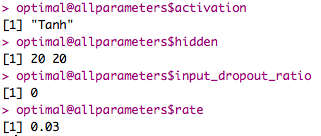
\includegraphics[scale = 0.7,angle = 0]{figure/optimalParam.png}
  \caption[Grid Model Parameters]{\normalsize{Grid Model Parameters}}
  \label{fig:Hyarn11}
  \end{figure}
  
  As shown by \autoref{fig:Hyarn122}, MSE on the optimal model for the
  training data was 6630.62 whereas MSE for the validation data was
  6883.68 and 6972.59 for the test data. The validation and test errors
  were higher than training signaling towards a good model fit, with some
  reservations for overfitting. Grid search model performs better than a
  simple deep model since the MSE for the validation and test data for
  grid search model (optimal) are lower than the MSE for the validation
  and test data for the original non-grid search model (deepmod)
  (validation MSE of 6918.5 and test MSE of 7010.6).
  
  \begin{figure}[htbp]
  \centering
  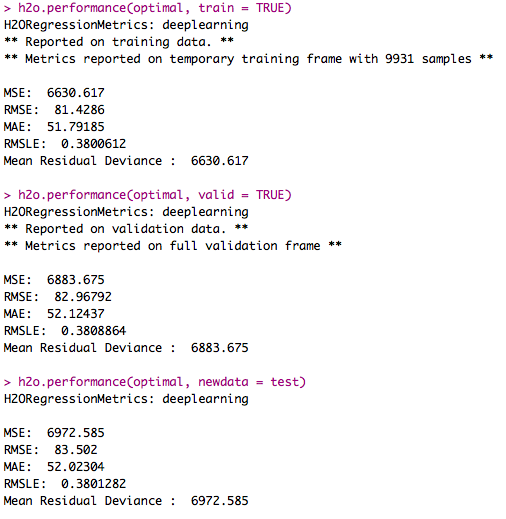
\includegraphics[scale = 0.8,angle = 0]{figure/DeepVarMod1.png}
  \caption[Grid Model Performance]{\normalsize{Grid Model Performance}}
  \label{fig:Hyarn122}
  \end{figure}
  
  Variable importance plot was used to view the most important predictors.
  As \autoref{fig:Hyarn89} shows, hour was most important in predicting
  departure delay greater than 90 minutes. Hour 6 and 5 am along with 9 pm
  were also important. Carriers Southwest (WN) and JetBlue (B6), weekday
  status of a weekend, season being summer and weekday being Friday were
  additionally important in predicting departure delay over 90 minutes.
  
  \begin{Shaded}
  \begin{Highlighting}[]
  \KeywordTok{h2o.varimp_plot}\NormalTok{(optimal, }\DataTypeTok{num_of_features =} \DecValTok{20}\NormalTok{)}
  \end{Highlighting}
  \end{Shaded}
  
  \begin{figure}[htbp]
  \centering
  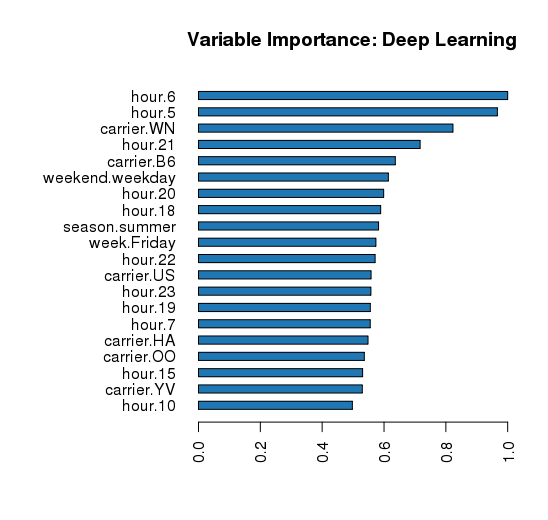
\includegraphics[scale = 1,angle = 0]{figure/VarModGrid.png}
  \caption[Grid Search Variable Importance]{\normalsize{Grid Search Variable Importance}}
  \label{fig:Hyarn89}
  \end{figure}
  
  \clearpage 
  
  \section{Random Grid Search Model}\label{random-grid-search-model}
  
  In comparison to grid search which iterated over parameter combinations
  exhaustively and sequentially, random grid search model was used to
  accelerate hyperparameter selection process. Random grid search proceeds
  to randomly search the user specified space based on established search
  criteria. Since random grid search model was used, additional
  hyperparameters were assessed for analysis. As shown below, Tanh and
  TanhWithDropout functions were tested. The hidden layer additionally
  included (30,30,30), (50,50) and (70,70). Rate 0.03 was tested along
  with 0.0 and 0.02. In addition, various combinations of regularization
  parameters (l1 and l2) were tested.
  
  \begin{Shaded}
  \begin{Highlighting}[]
  \NormalTok{hyper_params <-}\StringTok{ }\KeywordTok{list}\NormalTok{(}
    \DataTypeTok{activation=}\KeywordTok{c}\NormalTok{(}\StringTok{"Tanh"}\NormalTok{,}\StringTok{"TanhWithDropout"}\NormalTok{),}
    \DataTypeTok{hidden=}\KeywordTok{list}\NormalTok{(}\KeywordTok{c}\NormalTok{(}\DecValTok{20}\NormalTok{,}\DecValTok{20}\NormalTok{),}\KeywordTok{c}\NormalTok{(}\DecValTok{30}\NormalTok{,}\DecValTok{30}\NormalTok{,}\DecValTok{30}\NormalTok{),}\KeywordTok{c}\NormalTok{(}\DecValTok{40}\NormalTok{,}\DecValTok{40}\NormalTok{,}\DecValTok{40}\NormalTok{),}\KeywordTok{c}\NormalTok{(}\DecValTok{50}\NormalTok{,}\DecValTok{50}\NormalTok{),}\KeywordTok{c}\NormalTok{(}\DecValTok{70}\NormalTok{,}\DecValTok{70}\NormalTok{)),}
    \DataTypeTok{input_dropout_ratio=}\KeywordTok{c}\NormalTok{(}\DecValTok{0}\NormalTok{,}\FloatTok{0.05}\NormalTok{),}
    \DataTypeTok{rate=}\KeywordTok{c}\NormalTok{(}\FloatTok{0.01}\NormalTok{,}\FloatTok{0.02}\NormalTok{,}\FloatTok{0.03}\NormalTok{),}
    \DataTypeTok{l1=}\KeywordTok{seq}\NormalTok{(}\DecValTok{0}\NormalTok{,}\FloatTok{1e-4}\NormalTok{,}\FloatTok{1e-6}\NormalTok{),}
    \DataTypeTok{l2=}\KeywordTok{seq}\NormalTok{(}\DecValTok{0}\NormalTok{,}\FloatTok{1e-4}\NormalTok{,}\FloatTok{1e-6}\NormalTok{)}
  \NormalTok{)}
  \end{Highlighting}
  \end{Shaded}
  
  With the hyperparameters specified, next step included defining the
  search criteria. As the criteria below shows, the algorithm was defined
  to stop when the top 5 models were within 2\% of each other. Max model
  running time was 600 seconds (10 minutes). In addition to the max
  running time, number of max\_models can also be specified.
  
  \begin{Shaded}
  \begin{Highlighting}[]
  \NormalTok{search_criteria =}\StringTok{ }\KeywordTok{list}\NormalTok{(}\DataTypeTok{strategy =} \StringTok{"RandomDiscrete"}\NormalTok{, }
                         \DataTypeTok{max_runtime_secs =} \DecValTok{600}\NormalTok{, }\DataTypeTok{max_models =} \DecValTok{100}\NormalTok{, }
                         \DataTypeTok{seed=}\DecValTok{22}\NormalTok{, }\DataTypeTok{stopping_rounds=}\DecValTok{5}\NormalTok{, }
                         \DataTypeTok{stopping_tolerance=}\FloatTok{2e-2}\NormalTok{)}
  \end{Highlighting}
  \end{Shaded}
  
  Following delineation of the search criteria, the h2o.grid function was
  used to specify additional fixed parameters. Additional parameters
  included definition of epochs of 40, max\_w2 of 10,
  score\_validation\_samples of 10000 and score\_duty\_cycles of 0.025.
  The score\_validation\_samples specified the number of validation set
  samples for scoring while the score\_duty\_cycles specified the maximum
  duty cycle fraction for scoring. The same stopping parameters as the
  grid search model were used. The algorithm was thus indicated to stop
  when the MSE did not improve by at least 2\% for 2 scoring events.
  
  \begin{Shaded}
  \begin{Highlighting}[]
  \NormalTok{random_grid <-}\StringTok{ }\KeywordTok{h2o.grid}\NormalTok{(}
    \DataTypeTok{algorithm=}\StringTok{"deeplearning"}\NormalTok{,}
    \DataTypeTok{grid_id =} \StringTok{"Gridrandom"}\NormalTok{,}
    \DataTypeTok{training_frame=}\NormalTok{training,}
    \DataTypeTok{validation_frame=}\NormalTok{validation, }
    \DataTypeTok{x=}\NormalTok{myX, }
    \DataTypeTok{y=}\StringTok{"dep_delay"}\NormalTok{,}
    \DataTypeTok{epochs=}\DecValTok{40}\NormalTok{,}
    \DataTypeTok{stopping_metric=}\StringTok{"MSE"}\NormalTok{,}
    \DataTypeTok{stopping_tolerance=}\FloatTok{2e-2}\NormalTok{,        }
    \DataTypeTok{stopping_rounds=}\DecValTok{2}\NormalTok{,}
    \DataTypeTok{score_validation_samples=}\DecValTok{10000}\NormalTok{, }
    \DataTypeTok{score_duty_cycle=}\FloatTok{0.025}\NormalTok{,         }
    \DataTypeTok{max_w2=}\DecValTok{10}\NormalTok{,                      }
    \DataTypeTok{hyper_params =} \NormalTok{hyper_params,}
    \DataTypeTok{search_criteria =} \NormalTok{search_criteria}
  \NormalTok{)}
  \end{Highlighting}
  \end{Shaded}
  
  The validation set MSE for all random search models can be printed using
  for-loops. Additionally, the best model and its associated parameters
  can be viewed. As shown by \autoref{fig:Hyarn111}, optimal model
  generated by random grid search had an activation function of Tanh,
  hidden layer of (40, 40, 40), input\_dropout\_ratio of 0, rate of 0.03,
  l1 of 4.4e-05 and l2 of 7.4e-05.
  
  \begin{Shaded}
  \begin{Highlighting}[]
  \NormalTok{for (model_id in grid@model_ids) \{}
    \NormalTok{model <-}\StringTok{ }\KeywordTok{h2o.getModel}\NormalTok{(model_id)}
    \NormalTok{mse <-}\StringTok{ }\KeywordTok{h2o.mse}\NormalTok{(model, }\DataTypeTok{valid =} \OtherTok{TRUE}\NormalTok{) }
    \KeywordTok{sprintf}\NormalTok{(}\StringTok{"Validation set MSE: %f"}\NormalTok{, mse)}
  \NormalTok{\}}
  
  \CommentTok{#Retrieve optimal model by MSE}
  \NormalTok{grid@summary_table[}\DecValTok{1}\NormalTok{,] }
  \NormalTok{optimalRand <-}\StringTok{ }\KeywordTok{h2o.getModel}\NormalTok{(grid@model_ids[[}\DecValTok{1}\NormalTok{]]) }
  
  \NormalTok{optimalRand@allparameters }\CommentTok{#print all parameters of best model }
  \KeywordTok{h2o.performance}\NormalTok{(optimalRand, }\DataTypeTok{train =} \OtherTok{TRUE}\NormalTok{) }\CommentTok{#retrieve training MSE}
  \KeywordTok{h2o.performance}\NormalTok{(optimalRand, }\DataTypeTok{valid =} \OtherTok{TRUE}\NormalTok{) }\CommentTok{#retrieve validation MSE}
  \KeywordTok{h2o.performance}\NormalTok{(optimalRand, }\DataTypeTok{newdata =} \NormalTok{test) }\CommentTok{#retrieve test MSE }
  \end{Highlighting}
  \end{Shaded}
  
  \begin{figure}[htbp]
  \centering
  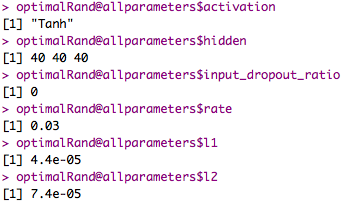
\includegraphics[scale = 0.7,angle = 0]{figure/optimRandomParam.png}
  \caption[Random Grid Model Parameters]{\normalsize{Random Grid Model Parameters}}
  \label{fig:Hyarn111}
  \end{figure}
  
  As \autoref{fig:Hyarn124} indicates, the MSE on the optimal random model
  for the training data was 6560.97 whereas MSE for the validation set was
  6577.3 and 6966.74 for the test set. The training, validation and test
  errors were lower than those yielded by the grid search model (6630.62
  for training, 6883.68 for validation and 6972.59 for test). The
  difference between the MSE for the validation and test set raised
  concerns about overfitting. The errors for the random search model were
  lower than the initial deep learning model deepmod validation and test
  errors (validation MSE of 6918.5 and test MSE of 7010.6).
  
  \begin{figure}[htbp]
  \centering
  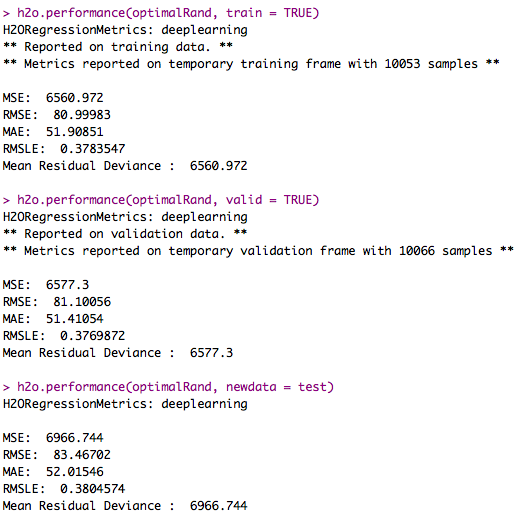
\includegraphics[scale = 0.8,angle = 0]{figure/DeepGridPerformRand.png}
  \caption[Random Grid Performance]{\normalsize{Random Grid Performance}}
  \label{fig:Hyarn124}
  \end{figure}
  
  Variable importance plot can be used to view the most important
  predictors. In this case, a plot of the top 20 predictors was produced.
  As \autoref{fig:Hyarn139} shows, carrier Hawaiian Airlines (HA) were
  most important at predicting departure delay greater than 90 minutes, a
  result corroborated by shiny app. Additionally hour (5, 6 and 9 am)and
  carrier (SkyWest Airlines (OO), Northwest Airlines (NW) and US Airways
  (US)) appeared to be important predictors of departure delay greater
  than 90 minutes.
  
  \begin{Shaded}
  \begin{Highlighting}[]
  \KeywordTok{h2o.varimp_plot}\NormalTok{(optimal, }\DataTypeTok{num_of_features =} \DecValTok{20}\NormalTok{)}
  \end{Highlighting}
  \end{Shaded}
  
  \begin{figure}[htbp]
  \centering
  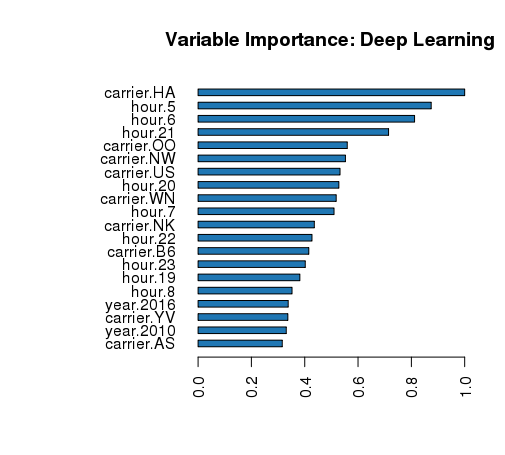
\includegraphics[scale = 1,angle = 0]{figure/VarGridRandom.png}
  \caption[Random Grid Variable Importance]{\normalsize{Random Grid Variable Importance}}
  \label{fig:Hyarn139}
  \end{figure}
  
  \clearpage 
  
  \section{Checkpoint Model}\label{checkpoint-model}
  
  Checkpoint functionality can be used in H2O to continue iterations from
  a previously built model. Checkpoint option allows specification of a
  previously built model key. The new model is then built as a
  continuation of the old model. If the model key is not supplied, then a
  new model is built instead. In the checkpoint model, the value of the
  parameters must be greater than their value set in the previous model.
  Parameters like activation function, max\_categorical\_features,
  momentum\_ramp, momentum\_stable, momentum\_start and nfolds cannot be
  modified. A full list of all the parameters that cannot be modified can
  be found at
  (\url{http://docs.h2o.ai/h2o/latest-stable/h2o-docs/data-science/algo-params/checkpoint.html})\footnote{(``Checkpoint,''
    n.d.)}.
  
  With some reservations about overfitting in the random grid search
  model, higher l1 and l2 parameters were used to see if better performing
  model can be produced than the random grid search model. Additionally
  higher epochs (50) was specified. These additional parameters were
  specified from the initial basis of the optimal random grid search
  model, specified below in the checkpoint specification as
  Gridrandom6\_model\_6. Same activation (Tanh), hidden layer (40, 40, 40)
  and rate (0.03) were used since these parameters can't be altered in the
  checkpoint model.
  
  \begin{Shaded}
  \begin{Highlighting}[]
  \NormalTok{max_epochs <-}\StringTok{ }\DecValTok{50} 
  \NormalTok{checkpoint <-}\StringTok{ }\KeywordTok{h2o.deeplearning}\NormalTok{(}
    \DataTypeTok{model_id=}\StringTok{"GridModRandom_continued2"}\NormalTok{, }
    \DataTypeTok{activation=}\StringTok{"Tanh"}\NormalTok{,}
    \DataTypeTok{checkpoint=}\StringTok{"Gridrandom6_model_6"}\NormalTok{, }
    \DataTypeTok{training_frame=}\NormalTok{training, }
    \DataTypeTok{validation_frame=}\NormalTok{validation, }
    \DataTypeTok{y=}\StringTok{"dep_delay"}\NormalTok{,}
    \DataTypeTok{x=}\NormalTok{myX, }
    \DataTypeTok{hidden=}\KeywordTok{c}\NormalTok{(}\DecValTok{40}\NormalTok{, }\DecValTok{40}\NormalTok{, }\DecValTok{40}\NormalTok{),          }
    \DataTypeTok{epochs=}\NormalTok{max_epochs,              }
    \DataTypeTok{stopping_metric=}\StringTok{"MSE"}\NormalTok{,     }
    \DataTypeTok{stopping_tolerance=}\FloatTok{2e-2}\NormalTok{,       }
    \DataTypeTok{stopping_rounds=}\DecValTok{2}\NormalTok{,}
    \DataTypeTok{score_duty_cycle=}\FloatTok{0.025}\NormalTok{,         }
    \DataTypeTok{adaptive_rate=}\NormalTok{T,                }
    \DataTypeTok{l1=}\FloatTok{1e-4}\NormalTok{,                        }
    \DataTypeTok{l2=}\FloatTok{1e-4}\NormalTok{,}
    \DataTypeTok{max_w2=}\DecValTok{10}\NormalTok{,}
    \DataTypeTok{rate =} \FloatTok{0.03}\NormalTok{,}
    \DataTypeTok{variable_importances=}\NormalTok{T}
  \NormalTok{) }
  \end{Highlighting}
  \end{Shaded}
  
  As shown by \autoref{fig:Hyarn143}, MSE on the training data was
  6874.65, 6899.89 for validation and 6992.02 for test data. Though the
  test set MSE for the checkpoint model is higher than the test MSE
  produced by the random grid model, the test MSE for the checkpoint model
  is closer to the validation set than the MSE for the validation and test
  sets in the model produced by random search grid criteria. The
  checkpoint model thus seems to have produced a better fitting model with
  reduced chance of overfitting than the random grid search model.
  
  \begin{figure}[htbp]
  \centering
  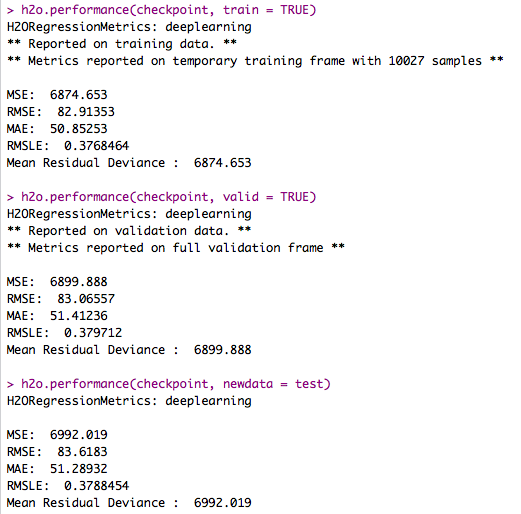
\includegraphics[scale = 0.7,angle = 0]{figure/DeepGridCheckpoint.png}
  \caption[Checkpoint Performance]{\normalsize{Checkpoint Performance}}
  \label{fig:Hyarn143}
  \end{figure}
  
  The variable importance plot shown in \autoref{fig:Hyarn17}, is
  comparable to the variable importance plot produced by random grid
  search model. Hawaiian carrier, 5 am, 6 am and 9 pm appeared to be the
  most important predictors of departure delay greater than 90 minutes.
  Additionally SkyWest Airlines, Northwest Airlines and US Airways
  appeared to be next important in predicting departure delay greater than
  90 minutes.
  
  \begin{figure}[htbp]
  \centering
  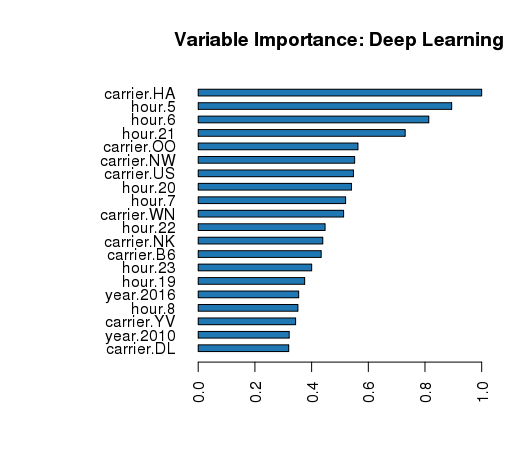
\includegraphics[scale = 0.9,angle = 0]{figure/VarImportCheckpoint.png}
  \caption[Checkpoint Variable Importance]{\normalsize{Checkpoint Variable Importance}}
  \label{fig:Hyarn17}
  \end{figure}
  
  \clearpage 
  
  \section{Conclusions}\label{conclusions}
  
  This chapter discussed deep learning models including concepts like
  setting up hyperparameters for deep learning models through the grid
  search and random search methods. In addition, the checkpoint model
  functionality was discussed.
  
  Overall, hour and carrier status predictors were most important
  predictors of departure delay greater than 90 minutes. Hour 5 am, 6 am,
  9 pm along with carriers Hawaiian Airlines, Northwest, Skywest, US
  Airlines, Southwest and JetBlue were also important.
  
  In regards to model performance, the grid search and the random grid
  model both performed better than the initial deep learning model. In
  addition, the checkpoint model reduced overfitting, thereby producing
  better performance than the random grid model.
  
  \chapter*{Conclusion}\label{conclusion-2}
  \addcontentsline{toc}{chapter}{Conclusion}
  
  This project assessed departure delay from 2008 to 2016. It involved
  navigation of both the R and Hadoop servers and utilized packages like
  h2o and rsparkling amongst others. Shiny application was used for
  initial data visualization. H2O platform was used to perform logistic
  modeling and deep learning. Logistic regression was performed with
  binary departure delay indicator variable (categorized by whether or not
  departure delay was over 30 minutes). In comparison, deep learning was
  performed with a continuous indicator of departure delay with data
  filtered for all flights with departure delay greater than 90 minutes.
  As described in the Deep Learning chapter, criteria of 30 minutes was
  chosen for logistic regression since it provided an adequate number of
  observations that either experienced or did not experience departure
  delay higher than 30 minutes. In comparison, a more stringent criteria
  of 90 minutes was used to model departure delay in neural network model
  since the interest was in modeling higher departure delay, which
  typically results in greater inconvenience. Weather was also assessed
  via logistic regression. Conceptually, this project explored big data
  infrastructure of platforms like Hadoop and Apache Spark, algorithms
  like neural networks and model optimization through grid and random
  based hyperparameter specification.
  
  \section{Limitation}\label{limitation}
  
  A limitation of this study was that although the original flights
  dataset had about a million observations, only a sample of about 200,000
  observations was copied in the Spark environment. Capacity of Spark can
  be improved to handle additional data. Parallel computing through the
  parallel package can be used to split the original data in smaller
  datasets followed by a computation aggregation.
  
  \section{Future Work}\label{future-work}
  
  Future extensions of this project can include building data pipelines to
  dynamically collect and study weather data for the associated flights.
  Data containing security alerts can also be used to gauge whether flight
  delays have been associated with increased alerts. Data on computer
  glitches and technical abnormalities as related to departure delay would
  also be insightful. Additionally, data on plane manufacturer can be
  obtained to gauge whether or not the extent of departure delay
  experienced by a plane is associated with its manufacture information.
  
  \appendix
  
  \chapter{Appendix}\label{appendix}
  
  \subsubsection{Creation of the FullDat dataset (flights data from 2008
  to
  2016)}\label{creation-of-the-fulldat-dataset-flights-data-from-2008-to-2016}
  
  \begin{Shaded}
  \begin{Highlighting}[]
  \KeywordTok{library}\NormalTok{(sparklyr)}
  \KeywordTok{library}\NormalTok{(rsparkling)}
  \KeywordTok{library}\NormalTok{(dplyr)}
  \KeywordTok{library}\NormalTok{(h2o)}
  
  \KeywordTok{options}\NormalTok{(}\DataTypeTok{rsparkling.sparklingwater.version =} \StringTok{"1.6.8"}\NormalTok{)}
  
  \NormalTok{sc <-}
  \KeywordTok{spark_connect}\NormalTok{(}\DataTypeTok{master =} \StringTok{"yarn-client"}\NormalTok{) }\CommentTok{#connecting to the cluster.}
  \CommentTok{#spark_disconnect(sc) disconnect to cluster}
  
  \CommentTok{#loading in flights dataset from 2008 to 2016}
  \NormalTok{flights2008 <-}
  \KeywordTok{spark_read_csv}\NormalTok{(}
  \NormalTok{sc,}
  \StringTok{"flights"}\NormalTok{,}
  \StringTok{"hdfs:///stats/nycflights}
  \StringTok{/flights/2008/part-m-*"}\NormalTok{,}
  \DataTypeTok{header =} \OtherTok{FALSE}\NormalTok{,}
  \DataTypeTok{memory =} \OtherTok{FALSE}
  \NormalTok{)}
  \NormalTok{flights2009 <-}
  \KeywordTok{spark_read_csv}\NormalTok{(}
  \NormalTok{sc,}
  \StringTok{"flights"}\NormalTok{,}
  \StringTok{"hdfs:///stats/nycflights}
  \StringTok{/flights/2009/part-m-*"}\NormalTok{,}
  \DataTypeTok{header =} \OtherTok{FALSE}\NormalTok{,}
  \DataTypeTok{memory =} \OtherTok{FALSE}
  \NormalTok{)}
  \NormalTok{flights2010 <-}
  \KeywordTok{spark_read_csv}\NormalTok{(}
  \NormalTok{sc,}
  \StringTok{"flights"}\NormalTok{,}
  \StringTok{"hdfs:///stats/nycflights}
  \StringTok{/flights/2010/part-m-*"}\NormalTok{,}
  \DataTypeTok{header =} \OtherTok{FALSE}\NormalTok{,}
  \DataTypeTok{memory =} \OtherTok{FALSE}
  \NormalTok{)}
  \NormalTok{flights2011 <-}
  \KeywordTok{spark_read_csv}\NormalTok{(}
  \NormalTok{sc,}
  \StringTok{"flights"}\NormalTok{,}
  \StringTok{"hdfs:///stats/nycflights}
  \StringTok{/flights/2011/part-m-*"}\NormalTok{,}
  \DataTypeTok{header =} \OtherTok{FALSE}\NormalTok{,}
  \DataTypeTok{memory =} \OtherTok{FALSE}
  \NormalTok{)}
  \NormalTok{flights2012 <-}
  \KeywordTok{spark_read_csv}\NormalTok{(}
  \NormalTok{sc,}
  \StringTok{"flights"}\NormalTok{,}
  \StringTok{"hdfs:///stats/nycflights}
  \StringTok{/flights/2012/part-m-*"}\NormalTok{,}
  \DataTypeTok{header =} \OtherTok{FALSE}\NormalTok{,}
  \DataTypeTok{memory =} \OtherTok{FALSE}
  \NormalTok{)}
  \NormalTok{flights2013 <-}
  \KeywordTok{spark_read_csv}\NormalTok{(}
  \NormalTok{sc,}
  \StringTok{"flights"}\NormalTok{,}
  \StringTok{"hdfs:///stats/nycflights}
  \StringTok{/flights/2013/part-m-*"}\NormalTok{,}
  \DataTypeTok{header =} \OtherTok{FALSE}\NormalTok{,}
  \DataTypeTok{memory =} \OtherTok{FALSE}
  \NormalTok{)}
  \NormalTok{flights2014 <-}
  \KeywordTok{spark_read_csv}\NormalTok{(}
  \NormalTok{sc,}
  \StringTok{"flights"}\NormalTok{,}
  \StringTok{"hdfs:///stats/nycflights}
  \StringTok{/flights/2014/part-m-*"}\NormalTok{,}
  \DataTypeTok{header =} \OtherTok{FALSE}\NormalTok{,}
  \DataTypeTok{memory =} \OtherTok{FALSE}
  \NormalTok{)}
  \NormalTok{flights2015 <-}
  \KeywordTok{spark_read_csv}\NormalTok{(}
  \NormalTok{sc,}
  \StringTok{"flights"}\NormalTok{,}
  \StringTok{"hdfs:///stats/nycflights}
  \StringTok{/flights/2015/part-m-*"}\NormalTok{,}
  \DataTypeTok{header =} \OtherTok{FALSE}\NormalTok{,}
  \DataTypeTok{memory =} \OtherTok{FALSE}
  \NormalTok{)}
  \NormalTok{flights2016 <-}
  \KeywordTok{spark_read_csv}\NormalTok{(}
  \NormalTok{sc,}
  \StringTok{"flights"}\NormalTok{,}
  \StringTok{"hdfs:///stats/nycflights}
  \StringTok{/flights/2016/part-m-*"}\NormalTok{,}
  \DataTypeTok{header =} \OtherTok{FALSE}\NormalTok{,}
  \DataTypeTok{memory =} \OtherTok{FALSE}
  \NormalTok{)}
  
  \CommentTok{#Columns were named}
  \NormalTok{flights2008 <-}\StringTok{ }\NormalTok{flights2008 %>%}
  \KeywordTok{rename}\NormalTok{(}\DataTypeTok{year =} \NormalTok{V1) %>%}
  \KeywordTok{rename}\NormalTok{(}\DataTypeTok{month =} \NormalTok{V2) %>%}
  \KeywordTok{rename}\NormalTok{(}\DataTypeTok{day =} \NormalTok{V3) %>%}
  \KeywordTok{rename}\NormalTok{(}\DataTypeTok{dep_time =} \NormalTok{V4) %>%}
  \KeywordTok{rename}\NormalTok{(}\DataTypeTok{sched_dep_time =} \NormalTok{V5) %>%}
  \KeywordTok{rename}\NormalTok{(}\DataTypeTok{dep_delay =} \NormalTok{V6) %>%}
  \KeywordTok{rename}\NormalTok{(}\DataTypeTok{arr_time =} \NormalTok{V7) %>%}
  \KeywordTok{rename}\NormalTok{(}\DataTypeTok{sched_arr_time =} \NormalTok{V8) %>%}
  \KeywordTok{rename}\NormalTok{(}\DataTypeTok{arr_delay =} \NormalTok{V9) %>%}
  \KeywordTok{rename}\NormalTok{(}\DataTypeTok{carrier =} \NormalTok{V10) %>%}
  \KeywordTok{rename}\NormalTok{(}\DataTypeTok{tailnum =} \NormalTok{V11) %>%}
  \KeywordTok{rename}\NormalTok{(}\DataTypeTok{flight =} \NormalTok{V12) %>%}
  \KeywordTok{rename}\NormalTok{(}\DataTypeTok{origin =} \NormalTok{V13) %>%}
  \KeywordTok{rename}\NormalTok{(}\DataTypeTok{dest =} \NormalTok{V14) %>%}
  \KeywordTok{rename}\NormalTok{(}\DataTypeTok{air_time =} \NormalTok{V15) %>%}
  \KeywordTok{rename}\NormalTok{(}\DataTypeTok{distance =} \NormalTok{V16) %>%}
  \KeywordTok{rename}\NormalTok{(}\DataTypeTok{hour =} \NormalTok{V18) %>%}
  \KeywordTok{rename}\NormalTok{(}\DataTypeTok{minute =} \NormalTok{V19) %>%}
  \KeywordTok{rename}\NormalTok{(}\DataTypeTok{time_hour =} \NormalTok{V20)}
  
  \CommentTok{#repeat this step for 2009-2016.}
  \KeywordTok{save}\NormalTok{(flights2008, }\DataTypeTok{file =} \StringTok{"Flights08.Rda"}\NormalTok{)}
  
  \KeywordTok{load}\NormalTok{(}\StringTok{"Flights08.Rda"}\NormalTok{)}
  \KeywordTok{load}\NormalTok{(}\StringTok{"Flights09.Rda"}\NormalTok{)}
  \KeywordTok{load}\NormalTok{(}\StringTok{"Flights10.Rda"}\NormalTok{)}
  \KeywordTok{load}\NormalTok{(}\StringTok{"Flights11.Rda"}\NormalTok{)}
  \KeywordTok{load}\NormalTok{(}\StringTok{"Flights12.Rda"}\NormalTok{)}
  \KeywordTok{load}\NormalTok{(}\StringTok{"Flights13.Rda"}\NormalTok{)}
  \KeywordTok{load}\NormalTok{(}\StringTok{"Flights14.Rda"}\NormalTok{)}
  \KeywordTok{load}\NormalTok{(}\StringTok{"Flights15.Rda"}\NormalTok{)}
  \KeywordTok{load}\NormalTok{(}\StringTok{"Flights16.Rda"}\NormalTok{)}
  
  \NormalTok{FinalDat <-}\StringTok{ }\KeywordTok{rbind}\NormalTok{(}
  \NormalTok{DatNew08,}
  \NormalTok{DatNew09,}
  \NormalTok{DatNew10,}
  \NormalTok{DatNew11,}
  \NormalTok{DatNew12,}
  \NormalTok{DatNew13,}
  \NormalTok{DatNew14,}
  \NormalTok{DatNew15,}
  \NormalTok{DatNew16}
  \NormalTok{)}
  \KeywordTok{save}\NormalTok{(FinalDat, }\DataTypeTok{file =} \StringTok{"FinalDataYear.Rda"}\NormalTok{)}
  \end{Highlighting}
  \end{Shaded}
  
  \subsubsection{H2O Logistic Regression}\label{h2o-logistic-regression}
  
  \begin{Shaded}
  \begin{Highlighting}[]
  \KeywordTok{library}\NormalTok{(sparklyr)}
  \KeywordTok{library}\NormalTok{(rsparkling)}
  \KeywordTok{library}\NormalTok{(dplyr)}
  \KeywordTok{library}\NormalTok{(h2o)}
  
  \KeywordTok{options}\NormalTok{(}\DataTypeTok{rsparkling.sparklingwater.version =} \StringTok{"1.6.8"}\NormalTok{)}
  \NormalTok{sc <-}\StringTok{ }\KeywordTok{spark_connect}\NormalTok{(}\DataTypeTok{master =} \StringTok{"yarn-client"}\NormalTok{)}
  
  \NormalTok{log <-}\StringTok{ }\KeywordTok{load}\NormalTok{(}\StringTok{"FullLogData.Rda"}\NormalTok{)}
  \NormalTok{datlog <-}\StringTok{ }\NormalTok{FullDatLog}
  
  \NormalTok{DatNew <-}\StringTok{ }\NormalTok{FullDatLog}
  \NormalTok{DatNew$hour <-}\StringTok{ }\KeywordTok{hour}\NormalTok{(}\KeywordTok{as.POSIXct}\NormalTok{(DatNew$time_hour))}
  \NormalTok{DatNew$week <-}\StringTok{ }\KeywordTok{weekdays}\NormalTok{(}\KeywordTok{as.Date}\NormalTok{(DatNew$time_hour))}
  \NormalTok{DatNew$hour <-}\StringTok{ }\KeywordTok{as.numeric}\NormalTok{(DatNew$hour)}
  \NormalTok{DatNew$hour <-}\StringTok{ }\KeywordTok{as.factor}\NormalTok{(DatNew$hour)}
  \NormalTok{DatNew$weekend <-}\StringTok{ }\KeywordTok{ifelse}\NormalTok{(DatNew$week %in%}\StringTok{ }\KeywordTok{c}\NormalTok{(}\StringTok{"Saturday"}\NormalTok{, }\StringTok{"Sunday"}\NormalTok{),}
  \StringTok{"weekend"}\NormalTok{, }\StringTok{"weekday"}\NormalTok{)}
  \NormalTok{data3 <-}\StringTok{ }\NormalTok{DatNew}
  \NormalTok{data3$carrier <-}\StringTok{ }\KeywordTok{as.character}\NormalTok{(data3$carrier)}
  
  
  \NormalTok{data3$weekend <-}\StringTok{ }\KeywordTok{as.factor}\NormalTok{(data3$weekend)}
  \NormalTok{data3$week <-}\StringTok{ }\KeywordTok{as.factor}\NormalTok{(data3$week)}
  \NormalTok{data3$carrier <-}\StringTok{ }\KeywordTok{as.factor}\NormalTok{(data3$carrier)}
  \NormalTok{data3$month <-}\StringTok{ }\KeywordTok{as.factor}\NormalTok{(data3$month)}
  \NormalTok{data3$month <-}\StringTok{ }\NormalTok{plyr::}\KeywordTok{mapvalues}\NormalTok{(}
  \NormalTok{data3$month,}
  \DataTypeTok{from =} \KeywordTok{c}\NormalTok{(}\StringTok{"1"}\NormalTok{, }\StringTok{"2"}\NormalTok{, }\StringTok{"3"}\NormalTok{,}
  \StringTok{"4"}\NormalTok{, }\StringTok{"5"}\NormalTok{, }\StringTok{"6"}\NormalTok{,}
  \StringTok{"7"}\NormalTok{, }\StringTok{"8"}\NormalTok{, }\StringTok{"9"}\NormalTok{,}
  \StringTok{"10"}\NormalTok{, }\StringTok{"11"}\NormalTok{, }\StringTok{"12"}\NormalTok{),}
  \DataTypeTok{to =} \KeywordTok{c}\NormalTok{(}
  \StringTok{"January"}\NormalTok{,}
  \StringTok{"February"}\NormalTok{,}
  \StringTok{"March"}\NormalTok{,}
  \StringTok{"April"}\NormalTok{,}
  \StringTok{"May"}\NormalTok{,}
  \StringTok{"June"}\NormalTok{,}
  \StringTok{"July"}\NormalTok{,}
  \StringTok{"August"}\NormalTok{,}
  \StringTok{"September"}\NormalTok{,}
  \StringTok{"October"}\NormalTok{,}
  \StringTok{"November"}\NormalTok{,}
  \StringTok{"December"}
  \NormalTok{)}
  \NormalTok{)}
  \NormalTok{data3$season <-}\StringTok{ }\KeywordTok{ifelse}\NormalTok{(}
  \NormalTok{data3$month %in%}\StringTok{ }\KeywordTok{c}\NormalTok{(}\StringTok{"March"}\NormalTok{, }\StringTok{"April"}\NormalTok{, }\StringTok{"May"}\NormalTok{),}
  \StringTok{"spring"}\NormalTok{,}
  \KeywordTok{ifelse}\NormalTok{(}
  \NormalTok{data3$month %in%}\StringTok{ }\KeywordTok{c}\NormalTok{(}\StringTok{"June"}\NormalTok{, }\StringTok{"July"}\NormalTok{,}
  \StringTok{"August"}\NormalTok{),}
  \StringTok{"summer"}\NormalTok{,}
  \KeywordTok{ifelse}\NormalTok{(}
  \NormalTok{data3$month %in%}\StringTok{ }\KeywordTok{c}\NormalTok{(}\StringTok{"September"}\NormalTok{,}
  \StringTok{"October"}\NormalTok{,}
  \StringTok{"November"}\NormalTok{),}
  \StringTok{"fall"}\NormalTok{,}
  \StringTok{"winter"}
  \NormalTok{)}
  \NormalTok{)}
  \NormalTok{)}
  
  \NormalTok{data3$season <-}\StringTok{ }\KeywordTok{as.factor}\NormalTok{(data3$season)}
  \NormalTok{data3$year <-}\StringTok{ }\KeywordTok{as.factor}\NormalTok{(data3$year)}
  \NormalTok{FullDatLog <-}\StringTok{ }\NormalTok{data3}
  
  \NormalTok{FullDatLog$year <-}\StringTok{ }\KeywordTok{as.factor}\NormalTok{(FullDatLog$year)}
  \NormalTok{FullDatLog$dep_delayIn =}\StringTok{ }\KeywordTok{ifelse}\NormalTok{(FullDatLog$dep_delay >}\StringTok{ }\DecValTok{30}\NormalTok{, }\StringTok{"Yes"}\NormalTok{, }\StringTok{"No"}\NormalTok{)}
  \NormalTok{FullDatLog$dep_delayIn <-}\StringTok{ }\KeywordTok{as.factor}\NormalTok{(FullDatLog$dep_delayIn)}
  \NormalTok{FullDatLog1 <-}\StringTok{ }\NormalTok{FullDatLog[}\KeywordTok{c}\NormalTok{(}\DecValTok{1}\NormalTok{, }\DecValTok{2}\NormalTok{, }\DecValTok{9}\NormalTok{, }\DecValTok{10}\NormalTok{, }\DecValTok{15}\NormalTok{, }\DecValTok{16}\NormalTok{, }\DecValTok{18}\NormalTok{, }\DecValTok{21}\NormalTok{, }\DecValTok{22}\NormalTok{, }\DecValTok{23}\NormalTok{, }\DecValTok{24}\NormalTok{)]}
  
  \NormalTok{FullDatLog <-}\StringTok{ }\NormalTok{FullDatLog1}
  \KeywordTok{save}\NormalTok{(FullDatLog, }\DataTypeTok{file =} \StringTok{"HadoopLogMod.Rda"}\NormalTok{)}
  
  \NormalTok{FullDatLog2 <-}\StringTok{ }\KeywordTok{load}\NormalTok{(}\StringTok{"HadoopLogMod.Rda"}\NormalTok{)}
  \KeywordTok{set.seed}\NormalTok{(}\DecValTok{134}\NormalTok{)}
  \NormalTok{sampled <-}
  \NormalTok{FullDatLog[}\KeywordTok{sample}\NormalTok{(}\KeywordTok{nrow}\NormalTok{(FullDatLog), }\DecValTok{200000}\NormalTok{, }\DataTypeTok{replace =} \OtherTok{FALSE}\NormalTok{,}
  \DataTypeTok{prob =} \OtherTok{NULL}\NormalTok{), ]}
  
  \NormalTok{mtcars_tbl <-}\StringTok{ }\KeywordTok{copy_to}\NormalTok{(sc, sampled, }\StringTok{"LogData"}\NormalTok{, }\DataTypeTok{overwrite =} \OtherTok{TRUE}\NormalTok{)}
  \NormalTok{partitions <-}\StringTok{ }\NormalTok{mtcars_tbl %>%}
  \KeywordTok{sdf_partition}\NormalTok{(}\DataTypeTok{training =} \FloatTok{0.75}\NormalTok{,}
  \DataTypeTok{test =} \FloatTok{0.25}\NormalTok{,}
  \DataTypeTok{seed =} \DecValTok{1099}\NormalTok{)}
  
  \NormalTok{training <-}\StringTok{ }\KeywordTok{as_h2o_frame}\NormalTok{(sc, partitions$training)}
  \NormalTok{test <-}\StringTok{ }\KeywordTok{as_h2o_frame}\NormalTok{(sc, partitions$test)}
  
  \NormalTok{training$dep_delayIn <-}\StringTok{ }\KeywordTok{as.factor}\NormalTok{(training$dep_delayIn)}
  \NormalTok{training$season <-}\StringTok{ }\KeywordTok{as.factor}\NormalTok{(training$season)}
  \NormalTok{training$week <-}\StringTok{ }\KeywordTok{as.factor}\NormalTok{(training$week)}
  \NormalTok{training$weekend <-}\StringTok{ }\KeywordTok{as.factor}\NormalTok{(training$weekend)}
  \NormalTok{training$carrier <-}\StringTok{ }\KeywordTok{as.factor}\NormalTok{(training$carrier)}
  \NormalTok{training$hour <-}\StringTok{ }\KeywordTok{as.factor}\NormalTok{(training$hour)}
  \NormalTok{training$month <-}\StringTok{ }\KeywordTok{as.factor}\NormalTok{(training$month)}
  \NormalTok{training$year <-}\StringTok{ }\KeywordTok{as.factor}\NormalTok{(training$year)}
  
  
  \NormalTok{test$dep_delayIn <-}\StringTok{ }\KeywordTok{as.factor}\NormalTok{(test$dep_delayIn)}
  \NormalTok{test$season <-}\StringTok{ }\KeywordTok{as.factor}\NormalTok{(test$season)}
  \NormalTok{test$week <-}\StringTok{ }\KeywordTok{as.factor}\NormalTok{(test$week)}
  \NormalTok{test$weekend <-}\StringTok{ }\KeywordTok{as.factor}\NormalTok{(test$weekend)}
  \NormalTok{test$carrier <-}\StringTok{ }\KeywordTok{as.factor}\NormalTok{(test$carrier)}
  \NormalTok{test$hour <-}\StringTok{ }\KeywordTok{as.factor}\NormalTok{(test$hour)}
  \NormalTok{test$month <-}\StringTok{ }\KeywordTok{as.factor}\NormalTok{(test$month)}
  \NormalTok{test$year <-}\StringTok{ }\KeywordTok{as.factor}\NormalTok{(test$year)}
  
  \NormalTok{myX =}\StringTok{ }\KeywordTok{setdiff}\NormalTok{(}\KeywordTok{colnames}\NormalTok{(training),}
  \KeywordTok{c}\NormalTok{(}\StringTok{"dep_delayIn"}\NormalTok{, }\StringTok{"orig_id"}\NormalTok{, }\StringTok{"hour"}\NormalTok{,}
  \StringTok{"month"}\NormalTok{, }\StringTok{"weekend"}\NormalTok{))}
  
  \NormalTok{regmod <-}\StringTok{ }\KeywordTok{h2o.glm}\NormalTok{(}
  \DataTypeTok{y =} \StringTok{"dep_delayIn"}\NormalTok{,}
  \DataTypeTok{x =} \NormalTok{myX,}
  \DataTypeTok{training_frame =} \NormalTok{training,}
  \DataTypeTok{family =} \StringTok{"binomial"}\NormalTok{,}
  \DataTypeTok{alpha =} \FloatTok{0.1}\NormalTok{,}
  \DataTypeTok{lambda_search =} \OtherTok{FALSE}\NormalTok{,}
  \DataTypeTok{nfolds =} \DecValTok{5}
  \NormalTok{)}
  
  \KeywordTok{h2o.performance}\NormalTok{(regmod)}
  \KeywordTok{h2o.varimp}\NormalTok{(regmod)}
  \KeywordTok{h2o.varimp_plot}\NormalTok{(regmod, }\DataTypeTok{num_of_features =} \DecValTok{20}\NormalTok{)}
  \NormalTok{mat <-}\StringTok{ }\KeywordTok{h2o.confusionMatrix}\NormalTok{(regmod)}
  \CommentTok{#model accuracy}
  \NormalTok{(mat$No[}\DecValTok{1}\NormalTok{] +}\StringTok{ }\NormalTok{mat$Yes[}\DecValTok{2}\NormalTok{]) /}\StringTok{ }\NormalTok{(mat$No[}\DecValTok{1}\NormalTok{] +}\StringTok{ }\NormalTok{mat$No[}\DecValTok{2}\NormalTok{] +}\StringTok{ }
  \StringTok{                              }\NormalTok{mat$Yes[}\DecValTok{1}\NormalTok{] +}\StringTok{ }\NormalTok{mat$Yes[}\DecValTok{2}\NormalTok{])}
  
  \NormalTok{pred <-}\StringTok{ }\KeywordTok{h2o.predict}\NormalTok{(}\DataTypeTok{object =} \NormalTok{regmod, }\DataTypeTok{newdata =} \NormalTok{test)}
  \KeywordTok{mean}\NormalTok{(pred$predict ==}\StringTok{ }\NormalTok{test$dep_delayIn)}
  \KeywordTok{plot}\NormalTok{(}\KeywordTok{h2o.performance}\NormalTok{(regmod))}
  
  \CommentTok{#Weather Logistic Regression}
  
  \NormalTok{flights$hour <-}\StringTok{ }\KeywordTok{ifelse}\NormalTok{(flights$hour ==}\StringTok{ }\DecValTok{24}\NormalTok{, }\DecValTok{0}\NormalTok{, flights$hour)}
  \NormalTok{flights_weather <-}\StringTok{ }\KeywordTok{left_join}\NormalTok{(flights, weather)}
  \NormalTok{flights_weather$total <-}\StringTok{ }\NormalTok{flights_weather$dep_delay +}
  \NormalTok{flights_weather$arr_delay}
  \NormalTok{flights_weather2 <-}\StringTok{ }\KeywordTok{filter}\NormalTok{(flights_weather, total >}\StringTok{ }\DecValTok{0}\NormalTok{)}
  
  \NormalTok{DatNew <-}\StringTok{ }\NormalTok{flights_weather2}
  \NormalTok{DatNew$hour <-}\StringTok{ }\KeywordTok{hour}\NormalTok{(}\KeywordTok{as.POSIXct}\NormalTok{(DatNew$time_hour))}
  \NormalTok{DatNew$week <-}\StringTok{ }\KeywordTok{weekdays}\NormalTok{(}\KeywordTok{as.Date}\NormalTok{(DatNew$time_hour))}
  \NormalTok{DatNew$hour <-}\StringTok{ }\KeywordTok{as.numeric}\NormalTok{(DatNew$hour)}
  \NormalTok{DatNew$hour <-}\StringTok{ }\KeywordTok{as.factor}\NormalTok{(DatNew$hour)}
  \NormalTok{DatNew$weekend <-}\StringTok{ }\KeywordTok{ifelse}\NormalTok{(DatNew$week %in%}\StringTok{ }\KeywordTok{c}\NormalTok{(}\StringTok{"Saturday"}\NormalTok{, }\StringTok{"Sunday"}\NormalTok{),}
  \StringTok{"weekend"}\NormalTok{, }\StringTok{"weekday"}\NormalTok{)}
  \NormalTok{DatNew$month <-}\StringTok{ }\KeywordTok{as.factor}\NormalTok{(DatNew$month)}
  \NormalTok{DatNew$month <-}
  \NormalTok{plyr::}\KeywordTok{mapvalues}\NormalTok{(}
  \NormalTok{DatNew$month,}
  \DataTypeTok{from =} \KeywordTok{c}\NormalTok{(}\StringTok{"1"}\NormalTok{, }\StringTok{"2"}\NormalTok{, }\StringTok{"3"}\NormalTok{,}
  \StringTok{"4"}\NormalTok{, }\StringTok{"5"}\NormalTok{, }\StringTok{"6"}\NormalTok{,}
  \StringTok{"7"}\NormalTok{, }\StringTok{"8"}\NormalTok{, }\StringTok{"9"}\NormalTok{,}
  \StringTok{"10"}\NormalTok{, }\StringTok{"11"}\NormalTok{, }\StringTok{"12"}\NormalTok{),}
  \DataTypeTok{to =} \KeywordTok{c}\NormalTok{(}
  \StringTok{"January"}\NormalTok{,}
  \StringTok{"February"}\NormalTok{,}
  \StringTok{"March"}\NormalTok{,}
  \StringTok{"April"}\NormalTok{,}
  \StringTok{"May"}\NormalTok{,}
  \StringTok{"June"}\NormalTok{,}
  \StringTok{"July"}\NormalTok{,}
  \StringTok{"August"}\NormalTok{,}
  \StringTok{"September"}\NormalTok{,}
  \StringTok{"October"}\NormalTok{,}
  \StringTok{"November"}\NormalTok{,}
  \StringTok{"December"}
  \NormalTok{)}
  \NormalTok{)}
  \NormalTok{DatNew$season <-}
  \KeywordTok{ifelse}\NormalTok{(}
  \NormalTok{DatNew$month %in%}\StringTok{ }\KeywordTok{c}\NormalTok{(}\StringTok{"March"}\NormalTok{, }\StringTok{"April"}\NormalTok{, }\StringTok{"May"}\NormalTok{),}
  \StringTok{"spring"}\NormalTok{,}
  \KeywordTok{ifelse}\NormalTok{(}
  \NormalTok{DatNew$month %in%}\StringTok{ }\KeywordTok{c}\NormalTok{(}\StringTok{"June"}\NormalTok{, }\StringTok{"July"}\NormalTok{,}
  \StringTok{"August"}\NormalTok{),}
  \StringTok{"summer"}\NormalTok{,}
  \KeywordTok{ifelse}\NormalTok{(}
  \NormalTok{DatNew$month %in%}\StringTok{ }\KeywordTok{c}\NormalTok{(}\StringTok{"September"}\NormalTok{,}
  \StringTok{"October"}\NormalTok{, }\StringTok{"November"}\NormalTok{),}
  \StringTok{"fall"}\NormalTok{,}
  \StringTok{"winter"}
  \NormalTok{)}
  \NormalTok{)}
  \NormalTok{)}
  
  \NormalTok{flights_weather2 <-}\StringTok{ }\NormalTok{DatNew}
  \KeywordTok{save}\NormalTok{(flights_weather2, }\DataTypeTok{file =} \StringTok{"flights_weather22.Rda"}\NormalTok{)}
  
  \KeywordTok{load}\NormalTok{(}\StringTok{"flights_weather22.Rda"}\NormalTok{)}
  \KeywordTok{head}\NormalTok{(flights_weather2)}
  \KeywordTok{names}\NormalTok{(flights_weather2)}
  \KeywordTok{nrow}\NormalTok{(flights_weather2)}
  \NormalTok{flights2 <-}\StringTok{ }\KeywordTok{na.omit}\NormalTok{(flights_weather2)}
  
  \NormalTok{mtcars_tbl <-}\StringTok{ }\KeywordTok{copy_to}\NormalTok{(sc, flights2, }\StringTok{"flights"}\NormalTok{, }\DataTypeTok{overwrite =} \OtherTok{TRUE}\NormalTok{)}
  \NormalTok{partitions <-}\StringTok{ }\NormalTok{mtcars_tbl %>%}
  \KeywordTok{sdf_partition}\NormalTok{(}\DataTypeTok{training =} \FloatTok{0.75}\NormalTok{,}
  \DataTypeTok{test =} \FloatTok{0.25}\NormalTok{,}
  \DataTypeTok{seed =} \DecValTok{1099}\NormalTok{)}
  
  \NormalTok{training <-}\StringTok{ }\KeywordTok{as_h2o_frame}\NormalTok{(sc, partitions$training)}
  \NormalTok{test <-}\StringTok{ }\KeywordTok{as_h2o_frame}\NormalTok{(sc, partitions$test)}
  
  \NormalTok{training$dep_delayIn <-}\StringTok{ }\KeywordTok{ifelse}\NormalTok{(training$dep_delay >}\StringTok{ }\DecValTok{30}\NormalTok{, }\StringTok{"Yes"}\NormalTok{, }\StringTok{"No"}\NormalTok{)}
  \NormalTok{test$dep_delayIn <-}\StringTok{ }\KeywordTok{ifelse}\NormalTok{(test$dep_delay >}\StringTok{ }\DecValTok{30}\NormalTok{, }\StringTok{"Yes"}\NormalTok{, }\StringTok{"No"}\NormalTok{)}
  
  \NormalTok{training$dep_delayIn <-}\StringTok{ }\KeywordTok{as.factor}\NormalTok{(training$dep_delayIn)}
  \NormalTok{training$season <-}\StringTok{ }\KeywordTok{as.factor}\NormalTok{(training$season)}
  \NormalTok{training$week <-}\StringTok{ }\KeywordTok{as.factor}\NormalTok{(training$week)}
  \NormalTok{training$weekend <-}\StringTok{ }\KeywordTok{as.factor}\NormalTok{(training$weekend)}
  \NormalTok{training$carrier <-}\StringTok{ }\KeywordTok{as.factor}\NormalTok{(training$carrier)}
  \NormalTok{training$hour <-}\StringTok{ }\KeywordTok{as.factor}\NormalTok{(training$hour)}
  \NormalTok{training$month <-}\StringTok{ }\KeywordTok{as.factor}\NormalTok{(training$month)}
  \NormalTok{training$year <-}\StringTok{ }\KeywordTok{as.factor}\NormalTok{(training$year)}
  \NormalTok{training$day <-}\StringTok{ }\KeywordTok{as.factor}\NormalTok{(training$day)}
  
  \NormalTok{test$dep_delayIn <-}\StringTok{ }\KeywordTok{as.factor}\NormalTok{(test$dep_delayIn)}
  \NormalTok{test$season <-}\StringTok{ }\KeywordTok{as.factor}\NormalTok{(test$season)}
  \NormalTok{test$week <-}\StringTok{ }\KeywordTok{as.factor}\NormalTok{(test$week)}
  \NormalTok{test$weekend <-}\StringTok{ }\KeywordTok{as.factor}\NormalTok{(test$weekend)}
  \NormalTok{test$carrier <-}\StringTok{ }\KeywordTok{as.factor}\NormalTok{(test$carrier)}
  \NormalTok{test$hour <-}\StringTok{ }\KeywordTok{as.factor}\NormalTok{(test$hour)}
  \NormalTok{test$month <-}\StringTok{ }\KeywordTok{as.factor}\NormalTok{(test$month)}
  \NormalTok{test$year <-}\StringTok{ }\KeywordTok{as.factor}\NormalTok{(test$year)}
  \NormalTok{test$day <-}\StringTok{ }\KeywordTok{as.factor}\NormalTok{(test$day)}
  
  \NormalTok{testDat <-}\StringTok{ }\NormalTok{test[, }\KeywordTok{c}\NormalTok{(}\DecValTok{1}\NormalTok{, }\DecValTok{2}\NormalTok{, }\DecValTok{3}\NormalTok{, }\DecValTok{9}\NormalTok{, }\DecValTok{10}\NormalTok{, }\DecValTok{15}\NormalTok{, }\DecValTok{16}\NormalTok{, }\DecValTok{17}\NormalTok{, }\DecValTok{20}\NormalTok{, }\DecValTok{21}\NormalTok{, }\DecValTok{22}\NormalTok{,}
  \DecValTok{23}\NormalTok{, }\DecValTok{24}\NormalTok{, }\DecValTok{25}\NormalTok{, }\DecValTok{26}\NormalTok{, }\DecValTok{27}\NormalTok{, }\DecValTok{28}\NormalTok{, }\DecValTok{30}\NormalTok{, }\DecValTok{31}\NormalTok{, }\DecValTok{32}\NormalTok{, }\DecValTok{33}\NormalTok{)]}
  \NormalTok{trainDat <-}\StringTok{ }\NormalTok{training[, }\KeywordTok{c}\NormalTok{(}\DecValTok{1}\NormalTok{, }\DecValTok{2}\NormalTok{, }\DecValTok{3}\NormalTok{, }\DecValTok{9}\NormalTok{, }\DecValTok{10}\NormalTok{, }\DecValTok{15}\NormalTok{, }\DecValTok{16}\NormalTok{, }\DecValTok{17}\NormalTok{, }\DecValTok{20}\NormalTok{, }\DecValTok{21}\NormalTok{, }\DecValTok{22}\NormalTok{,}
  \DecValTok{23}\NormalTok{, }\DecValTok{24}\NormalTok{, }\DecValTok{25}\NormalTok{, }\DecValTok{26}\NormalTok{, }\DecValTok{27}\NormalTok{, }\DecValTok{28}\NormalTok{, }\DecValTok{30}\NormalTok{, }\DecValTok{31}\NormalTok{, }\DecValTok{32}\NormalTok{, }\DecValTok{33}\NormalTok{)]}
  
  \NormalTok{myX =}\StringTok{ }\KeywordTok{setdiff}\NormalTok{(}\KeywordTok{colnames}\NormalTok{(testDat), }\KeywordTok{c}\NormalTok{(}\StringTok{"dep_delayIn"}\NormalTok{))}
  \NormalTok{regmod <-}\StringTok{ }\KeywordTok{h2o.glm}\NormalTok{(}
  \DataTypeTok{y =} \StringTok{"dep_delayIn"}\NormalTok{,}
  \DataTypeTok{x =} \NormalTok{myX,}
  \DataTypeTok{training_frame =} \NormalTok{trainDat,}
  \DataTypeTok{family =} \StringTok{"binomial"}\NormalTok{,}
  \DataTypeTok{alpha =} \FloatTok{0.1}\NormalTok{,}
  \DataTypeTok{lambda_search =} \OtherTok{FALSE}\NormalTok{,}
  \DataTypeTok{nfolds =} \DecValTok{5}
  \NormalTok{)}
  
  \NormalTok{regmodWeather <-}\StringTok{ }\NormalTok{regmod}
  \KeywordTok{h2o.performance}\NormalTok{(regmodWeather)}
  \KeywordTok{h2o.varimp}\NormalTok{(regmod)}
  \KeywordTok{h2o.varimp_plot}\NormalTok{(regmodWeather, }\DataTypeTok{num_of_features =} \DecValTok{30}\NormalTok{)}
  \KeywordTok{h2o.confusionMatrix}\NormalTok{(regmodWeather)}
  \NormalTok{(mat$No[}\DecValTok{1}\NormalTok{] +}\StringTok{ }\NormalTok{mat$Yes[}\DecValTok{2}\NormalTok{]) /}\StringTok{ }\NormalTok{(mat$No[}\DecValTok{1}\NormalTok{] +}\StringTok{ }\NormalTok{mat$No[}\DecValTok{2}\NormalTok{] +}\StringTok{ }
  \StringTok{                              }\NormalTok{mat$Yes[}\DecValTok{1}\NormalTok{] +}\StringTok{ }\NormalTok{mat$Yes[}\DecValTok{2}\NormalTok{])}
  
  \NormalTok{pred <-}\StringTok{ }\KeywordTok{h2o.predict}\NormalTok{(}\DataTypeTok{object =} \NormalTok{regmodWeather, }\DataTypeTok{newdata =} \NormalTok{testDat)}
  \KeywordTok{mean}\NormalTok{(pred$predict ==}\StringTok{ }\NormalTok{testDat$dep_delayIn) }\CommentTok{#accuracy of test set}
  \end{Highlighting}
  \end{Shaded}
  
  \subsubsection{H2O Deep Learning}\label{h2o-deep-learning-1}
  
  \begin{Shaded}
  \begin{Highlighting}[]
  \KeywordTok{library}\NormalTok{(sparklyr)}
  \KeywordTok{library}\NormalTok{(rsparkling)}
  \KeywordTok{library}\NormalTok{(dplyr)}
  \KeywordTok{library}\NormalTok{(h2o)}
  
   
  \KeywordTok{options}\NormalTok{(}\DataTypeTok{rsparkling.sparklingwater.version =} \StringTok{"1.6.8"}\NormalTok{)}
  \CommentTok{#spark_disconnect(sc)}
  \NormalTok{sc <-}\StringTok{ }\KeywordTok{spark_connect}\NormalTok{(}\DataTypeTok{master =} \StringTok{"yarn-client"}\NormalTok{) }
  
  \NormalTok{yas <-}\StringTok{ }\KeywordTok{load}\NormalTok{(}\StringTok{"FinalDataYear.Rda"}\NormalTok{)}
  \KeywordTok{head}\NormalTok{(FinalDat)}
  \KeywordTok{nrow}\NormalTok{(FinalDat)}
  \KeywordTok{unique}\NormalTok{(FinalDat$year)}
  
  \NormalTok{DatNew <-}\StringTok{ }\NormalTok{FinalDat}
  \NormalTok{DatNew$hour <-}\StringTok{ }\KeywordTok{hour}\NormalTok{(}\KeywordTok{as.POSIXct}\NormalTok{(DatNew$time_hour))}
  \NormalTok{DatNew$week <-}\StringTok{ }\KeywordTok{weekdays}\NormalTok{(}\KeywordTok{as.Date}\NormalTok{(DatNew$time_hour))}
  \NormalTok{DatNew$hour <-}\StringTok{ }\KeywordTok{as.numeric}\NormalTok{(DatNew$hour)}
  \NormalTok{DatNew$hour <-}\StringTok{ }\KeywordTok{as.factor}\NormalTok{(DatNew$hour)}
  \NormalTok{DatNew$weekend<-}\StringTok{ }\KeywordTok{ifelse}\NormalTok{(DatNew$week %in%}\StringTok{ }\KeywordTok{c}\NormalTok{(}\StringTok{"Saturday"}\NormalTok{, }\StringTok{"Sunday"}\NormalTok{), }
                          \StringTok{"weekend"}\NormalTok{,}\StringTok{"weekday"}\NormalTok{)}
  \NormalTok{data3 <-}\StringTok{ }\NormalTok{DatNew}
  \NormalTok{data3$carrier <-}\StringTok{ }\KeywordTok{as.character}\NormalTok{(data3$carrier)}
  
  
  \NormalTok{data3$weekend <-}\StringTok{ }\KeywordTok{as.factor}\NormalTok{(data3$weekend)}
  \NormalTok{data3$week <-}\StringTok{ }\KeywordTok{as.factor}\NormalTok{(data3$week)}
  \NormalTok{data3$carrier <-}\StringTok{ }\KeywordTok{as.factor}\NormalTok{(data3$carrier)}
  \NormalTok{data3$month <-}\StringTok{ }\KeywordTok{as.factor}\NormalTok{(data3$month)}
  \NormalTok{data3$month <-}\StringTok{ }\NormalTok{plyr::}\KeywordTok{mapvalues}\NormalTok{(data3$month, }
                                 \DataTypeTok{from =} \KeywordTok{c}\NormalTok{(}\StringTok{"1"}\NormalTok{, }\StringTok{"2"}\NormalTok{, }\StringTok{"3"}\NormalTok{, }
                                          \StringTok{"4"}\NormalTok{, }\StringTok{"5"}\NormalTok{, }\StringTok{"6"}\NormalTok{, }
                                          \StringTok{"7"}\NormalTok{, }\StringTok{"8"}\NormalTok{, }\StringTok{"9"}\NormalTok{, }
                                          \StringTok{"10"}\NormalTok{, }\StringTok{"11"}\NormalTok{, }\StringTok{"12"}\NormalTok{), }
                        \DataTypeTok{to =} \KeywordTok{c}\NormalTok{(}\StringTok{"January"}\NormalTok{, }\StringTok{"February"}\NormalTok{, }\StringTok{"March"}\NormalTok{, }
                              \StringTok{"April"}\NormalTok{, }\StringTok{"May"}\NormalTok{, }\StringTok{"June"}\NormalTok{, }\StringTok{"July"}\NormalTok{, }
                              \StringTok{"August"}\NormalTok{, }\StringTok{"September"}\NormalTok{, }
                              \StringTok{"October"}\NormalTok{, }\StringTok{"November"}\NormalTok{, }\StringTok{"December"}\NormalTok{))}
  \NormalTok{data3$season <-}\StringTok{ }\KeywordTok{ifelse}\NormalTok{(data3$month %in%}\StringTok{ }\KeywordTok{c}\NormalTok{(}\StringTok{"March"}\NormalTok{, }\StringTok{"April"}\NormalTok{, }\StringTok{"May"}\NormalTok{), }
                         \StringTok{"spring"}\NormalTok{, }
                         \KeywordTok{ifelse}\NormalTok{(data3$month %in%}\StringTok{ }\KeywordTok{c}\NormalTok{(}\StringTok{"June"}\NormalTok{, }\StringTok{"July"}\NormalTok{, }
                                                   \StringTok{"August"}\NormalTok{), }
                                \StringTok{"summer"}\NormalTok{, }
                                \KeywordTok{ifelse}\NormalTok{(data3$month %in%}\StringTok{ }\KeywordTok{c}\NormalTok{(}\StringTok{"September"}\NormalTok{, }
                                                          \StringTok{"October"}\NormalTok{, }
                                                          \StringTok{"November"}\NormalTok{), }
                                       \StringTok{"fall"}\NormalTok{, }\StringTok{"winter"}\NormalTok{)))}
  
  \NormalTok{data3$season <-}\StringTok{ }\KeywordTok{as.factor}\NormalTok{(data3$season)}
  \NormalTok{data3$year <-}\StringTok{ }\KeywordTok{as.factor}\NormalTok{(data3$year)}
  \NormalTok{FullDatLog <-}\StringTok{ }\NormalTok{data3}
  \NormalTok{FullDatLog$year <-}\StringTok{ }\KeywordTok{as.factor}\NormalTok{(FullDatLog$year)}
  \NormalTok{FullDatLog$dep_delay <-}\StringTok{ }\KeywordTok{as.numeric}\NormalTok{(FullDatLog$dep_delay)}
  \KeywordTok{nrow}\NormalTok{(FullDatLog)}
  
  \KeywordTok{set.seed}\NormalTok{(}\DecValTok{12}\NormalTok{) }
  \NormalTok{sampled <-}\StringTok{ }\NormalTok{FullDatLog[}\KeywordTok{sample}\NormalTok{(}\KeywordTok{nrow}\NormalTok{(FullDatLog), }
                                \DecValTok{200000}\NormalTok{, }\DataTypeTok{replace =} \OtherTok{FALSE}\NormalTok{, }\DataTypeTok{prob =} \OtherTok{NULL}\NormalTok{),]}
  \NormalTok{mtcars_tbl <-}\StringTok{ }\KeywordTok{copy_to}\NormalTok{(sc, sampled, }\StringTok{"deep"}\NormalTok{, }\DataTypeTok{overwrite =} \OtherTok{TRUE}\NormalTok{)  }
  \NormalTok{partitions <-}\StringTok{ }\NormalTok{mtcars_tbl %>%}
  \StringTok{  }\KeywordTok{sdf_partition}\NormalTok{(}\DataTypeTok{training =} \FloatTok{0.5}\NormalTok{, }\DataTypeTok{validation =} \FloatTok{0.25}\NormalTok{, }
                  \DataTypeTok{test =} \FloatTok{0.25}\NormalTok{, }\DataTypeTok{seed =} \DecValTok{1099}\NormalTok{)}
  
  \NormalTok{training <-}\StringTok{ }\KeywordTok{as_h2o_frame}\NormalTok{(sc, partitions$training)}
  \NormalTok{validation <-}\StringTok{ }\KeywordTok{as_h2o_frame}\NormalTok{(sc, partitions$validation)}
  \NormalTok{test <-}\StringTok{ }\KeywordTok{as_h2o_frame}\NormalTok{(sc, partitions$test)}
  
  \NormalTok{training$dep_delay <-}\StringTok{ }\KeywordTok{as.numeric}\NormalTok{(training$dep_delay)}
  \NormalTok{training$arr_delay <-}\StringTok{ }\KeywordTok{as.numeric}\NormalTok{(training$arr_delay)}
  \NormalTok{training$air_time <-}\StringTok{ }\KeywordTok{as.numeric}\NormalTok{(training$air_time)}
  \NormalTok{training$season <-}\StringTok{ }\KeywordTok{as.factor}\NormalTok{(training$season)}
  \NormalTok{training$week <-}\StringTok{ }\KeywordTok{as.factor}\NormalTok{(training$week)}
  \NormalTok{training$weekend <-}\StringTok{ }\KeywordTok{as.factor}\NormalTok{(training$weekend)}
  \NormalTok{training$carrier <-}\StringTok{ }\KeywordTok{as.factor}\NormalTok{(training$carrier)}
  \NormalTok{training$hour <-}\StringTok{ }\KeywordTok{as.factor}\NormalTok{(training$hour)}
  \NormalTok{training$month <-}\StringTok{ }\KeywordTok{as.factor}\NormalTok{(training$month)}
  \NormalTok{training$year <-}\StringTok{ }\KeywordTok{as.factor}\NormalTok{(training$year)}
  
  \NormalTok{validation$dep_delay <-}\StringTok{ }\KeywordTok{as.numeric}\NormalTok{(validation$dep_delay)}
  \NormalTok{validation$arr_delay <-}\StringTok{ }\KeywordTok{as.numeric}\NormalTok{(validation$arr_delay)}
  \NormalTok{validation$air_time <-}\StringTok{ }\KeywordTok{as.numeric}\NormalTok{(validation$air_time)}
  \NormalTok{validation$season <-}\StringTok{ }\KeywordTok{as.factor}\NormalTok{(validation$season)}
  \NormalTok{validation$week <-}\StringTok{ }\KeywordTok{as.factor}\NormalTok{(validation$week)}
  \NormalTok{validation$weekend <-}\StringTok{ }\KeywordTok{as.factor}\NormalTok{(validation$weekend)}
  \NormalTok{validation$carrier <-}\StringTok{ }\KeywordTok{as.factor}\NormalTok{(validation$carrier)}
  \NormalTok{validation$hour <-}\StringTok{ }\KeywordTok{as.factor}\NormalTok{(validation$hour)}
  \NormalTok{validation$month <-}\StringTok{ }\KeywordTok{as.factor}\NormalTok{(validation$month)}
  \NormalTok{validation$year <-}\StringTok{ }\KeywordTok{as.factor}\NormalTok{(validation$year)}
  
  \NormalTok{test$dep_delay <-}\StringTok{ }\KeywordTok{as.numeric}\NormalTok{(test$dep_delay)}
  \NormalTok{test$arr_delay <-}\StringTok{ }\KeywordTok{as.numeric}\NormalTok{(test$arr_delay)}
  \NormalTok{test$air_time <-}\StringTok{ }\KeywordTok{as.numeric}\NormalTok{(test$air_time)}
  \NormalTok{test$season <-}\StringTok{ }\KeywordTok{as.factor}\NormalTok{(test$season)}
  \NormalTok{test$week <-}\StringTok{ }\KeywordTok{as.factor}\NormalTok{(test$week)}
  \NormalTok{test$weekend <-}\StringTok{ }\KeywordTok{as.factor}\NormalTok{(test$weekend)}
  \NormalTok{test$carrier <-}\StringTok{ }\KeywordTok{as.factor}\NormalTok{(test$carrier)}
  \NormalTok{test$hour <-}\StringTok{ }\KeywordTok{as.factor}\NormalTok{(test$hour)}
  \NormalTok{test$month <-}\StringTok{ }\KeywordTok{as.factor}\NormalTok{(test$month)}
  \NormalTok{test$year <-}\StringTok{ }\KeywordTok{as.factor}\NormalTok{(test$year)}
  
  \NormalTok{training <-}\StringTok{ }\NormalTok{training[,}\KeywordTok{c}\NormalTok{(}\DecValTok{1}\NormalTok{,}\DecValTok{2}\NormalTok{,}\DecValTok{6}\NormalTok{,}\DecValTok{9}\NormalTok{,}\DecValTok{10}\NormalTok{,}\DecValTok{15}\NormalTok{,}\DecValTok{16}\NormalTok{,}\DecValTok{18}\NormalTok{,}\DecValTok{21}\NormalTok{,}\DecValTok{22}\NormalTok{,}\DecValTok{23}\NormalTok{)]}
  \NormalTok{test <-}\StringTok{ }\NormalTok{test[,}\KeywordTok{c}\NormalTok{(}\DecValTok{1}\NormalTok{,}\DecValTok{2}\NormalTok{,}\DecValTok{6}\NormalTok{,}\DecValTok{9}\NormalTok{,}\DecValTok{10}\NormalTok{,}\DecValTok{15}\NormalTok{,}\DecValTok{16}\NormalTok{,}\DecValTok{18}\NormalTok{,}\DecValTok{21}\NormalTok{,}\DecValTok{22}\NormalTok{,}\DecValTok{23}\NormalTok{)]}
  \NormalTok{validation <-}\StringTok{ }\NormalTok{validation[,}\KeywordTok{c}\NormalTok{(}\DecValTok{1}\NormalTok{,}\DecValTok{2}\NormalTok{,}\DecValTok{6}\NormalTok{,}\DecValTok{9}\NormalTok{,}\DecValTok{10}\NormalTok{,}\DecValTok{15}\NormalTok{,}\DecValTok{16}\NormalTok{,}\DecValTok{18}\NormalTok{,}\DecValTok{21}\NormalTok{,}\DecValTok{22}\NormalTok{,}\DecValTok{23}\NormalTok{)]}
  
  \NormalTok{myX =}\StringTok{ }\KeywordTok{setdiff}\NormalTok{(}\KeywordTok{colnames}\NormalTok{(training), (}\StringTok{"dep_delay"}\NormalTok{))}
  
  \CommentTok{#First simplified deep learning model }
  \NormalTok{m1 <-}\StringTok{ }\KeywordTok{h2o.deeplearning}\NormalTok{(}
    \DataTypeTok{y=}\StringTok{"dep_delay"}\NormalTok{,}
    \DataTypeTok{x=}\NormalTok{myX,}
    \DataTypeTok{activation=}\StringTok{"Tanh"}\NormalTok{,  }
    \DataTypeTok{training_frame=}\NormalTok{training, }
    \DataTypeTok{validation_frame=}\NormalTok{validation,}
    \DataTypeTok{epochs=}\DecValTok{1}\NormalTok{,}
    \DataTypeTok{variable_importances=}\NormalTok{T,    }
    \DataTypeTok{nfolds =} \DecValTok{5}\NormalTok{,}
    \DataTypeTok{keep_cross_validation_predictions=}\NormalTok{T}
  \NormalTok{)}
  
  \NormalTok{deepmod <-}\StringTok{ }\NormalTok{m1}
  \KeywordTok{h2o.performance}\NormalTok{(deepmod, }\DataTypeTok{train =} \OtherTok{TRUE}\NormalTok{)  }
  \KeywordTok{h2o.performance}\NormalTok{(deepmod, }\DataTypeTok{valid =} \OtherTok{TRUE}\NormalTok{) }
  \KeywordTok{h2o.performance}\NormalTok{(deepmod, }\DataTypeTok{newdata =} \NormalTok{test)}
  \KeywordTok{h2o.varimp_plot}\NormalTok{(deepmod, }\DataTypeTok{num_of_features =} \DecValTok{20}\NormalTok{)}
  
  \CommentTok{#Grid search model iteration }
  \NormalTok{hyper_params <-}\StringTok{ }\KeywordTok{list}\NormalTok{(}
    \DataTypeTok{activation=}\KeywordTok{c}\NormalTok{(}\StringTok{"Tanh"}\NormalTok{, }\StringTok{"TanhWithDropout"}\NormalTok{),}
    \DataTypeTok{hidden=}\KeywordTok{list}\NormalTok{(}\KeywordTok{c}\NormalTok{(}\DecValTok{20}\NormalTok{,}\DecValTok{20}\NormalTok{),}\KeywordTok{c}\NormalTok{(}\DecValTok{40}\NormalTok{,}\DecValTok{40}\NormalTok{)),}
    \DataTypeTok{input_dropout_ratio=}\KeywordTok{c}\NormalTok{(}\DecValTok{0}\NormalTok{,}\FloatTok{0.05}\NormalTok{),}
    \DataTypeTok{rate=}\KeywordTok{c}\NormalTok{(}\FloatTok{0.01}\NormalTok{,}\FloatTok{0.02}\NormalTok{,}\FloatTok{0.03}\NormalTok{)}
  \NormalTok{)}
  
  \NormalTok{grid <-}\StringTok{ }\KeywordTok{h2o.grid}\NormalTok{(}
    \DataTypeTok{algorithm=}\StringTok{"deeplearning"}\NormalTok{,}
    \DataTypeTok{grid_id=}\StringTok{"gridDeep"}\NormalTok{, }
    \DataTypeTok{training_frame=}\NormalTok{training,}
    \DataTypeTok{validation_frame=}\NormalTok{validation,}
    \DataTypeTok{y=}\StringTok{"dep_delay"}\NormalTok{,}
    \DataTypeTok{x=}\NormalTok{myX,}
    \DataTypeTok{epochs=}\DecValTok{10}\NormalTok{,}
    \DataTypeTok{stopping_metric=}\StringTok{"MSE"}\NormalTok{,}
    \DataTypeTok{stopping_tolerance=}\FloatTok{2e-2}\NormalTok{,        }
    \DataTypeTok{stopping_rounds=}\DecValTok{2}\NormalTok{, }
    \DataTypeTok{score_duty_cycle=}\FloatTok{0.025}\NormalTok{,         }
    \DataTypeTok{adaptive_rate=}\NormalTok{T,                }
    \DataTypeTok{momentum_start=}\FloatTok{0.5}\NormalTok{,             }
    \DataTypeTok{momentum_stable=}\FloatTok{0.9}\NormalTok{, }
    \DataTypeTok{momentum_ramp=}\FloatTok{1e7}\NormalTok{,}
    \DataTypeTok{variable_importances=}\NormalTok{T,}
    \DataTypeTok{l1=}\FloatTok{1e-5}\NormalTok{,                         }
    \DataTypeTok{l2=}\FloatTok{1e-5}\NormalTok{,}
    \DataTypeTok{max_w2=}\DecValTok{10}\NormalTok{, }
    \DataTypeTok{hyper_params=}\NormalTok{hyper_params}
  \NormalTok{)}
  
  \NormalTok{for (model_id in grid@model_ids) \{ }\CommentTok{#print model MSE}
    \NormalTok{model <-}\StringTok{ }\KeywordTok{h2o.getModel}\NormalTok{(model_id)}
    \NormalTok{mse <-}\StringTok{ }\KeywordTok{h2o.mse}\NormalTok{(model, }\DataTypeTok{valid =} \OtherTok{TRUE}\NormalTok{) }
    \KeywordTok{print}\NormalTok{(}\KeywordTok{sprintf}\NormalTok{(}\StringTok{"Validation set MSE: %f"}\NormalTok{, mse))}
  \NormalTok{\}}
  \NormalTok{grid@summary_table[}\DecValTok{1}\NormalTok{,] }
  \NormalTok{optimal <-}\StringTok{ }\KeywordTok{h2o.getModel}\NormalTok{(grid@model_ids[[}\DecValTok{1}\NormalTok{]]) }
  
  \NormalTok{optimal@allparameters }\CommentTok{#print all parameters of best model }
  \KeywordTok{h2o.performance}\NormalTok{(optimal, }\DataTypeTok{train =} \OtherTok{TRUE}\NormalTok{) }\CommentTok{#retrieve training MSE}
  \KeywordTok{h2o.performance}\NormalTok{(optimal, }\DataTypeTok{valid =} \OtherTok{TRUE}\NormalTok{) }\CommentTok{#retrieve validation MSE}
  \KeywordTok{h2o.performance}\NormalTok{(optimal, }\DataTypeTok{newdata =} \NormalTok{test) }\CommentTok{#retrieve test MSE }
  
  \KeywordTok{h2o.varimp_plot}\NormalTok{(optimal, }\DataTypeTok{num_of_features =} \DecValTok{20}\NormalTok{)}
  
  \CommentTok{#Random grid search model }
  \NormalTok{hyper_params <-}\StringTok{ }\KeywordTok{list}\NormalTok{(}
    \DataTypeTok{activation=}\KeywordTok{c}\NormalTok{(}\StringTok{"Tanh"}\NormalTok{,}\StringTok{"TanhWithDropout"}\NormalTok{),}
    \DataTypeTok{hidden=}\KeywordTok{list}\NormalTok{(}\KeywordTok{c}\NormalTok{(}\DecValTok{20}\NormalTok{,}\DecValTok{20}\NormalTok{),}\KeywordTok{c}\NormalTok{(}\DecValTok{30}\NormalTok{,}\DecValTok{30}\NormalTok{,}\DecValTok{30}\NormalTok{),}\KeywordTok{c}\NormalTok{(}\DecValTok{40}\NormalTok{,}\DecValTok{40}\NormalTok{,}\DecValTok{40}\NormalTok{),}
                \KeywordTok{c}\NormalTok{(}\DecValTok{50}\NormalTok{,}\DecValTok{50}\NormalTok{),}\KeywordTok{c}\NormalTok{(}\DecValTok{70}\NormalTok{,}\DecValTok{70}\NormalTok{)),}
    \DataTypeTok{input_dropout_ratio=}\KeywordTok{c}\NormalTok{(}\DecValTok{0}\NormalTok{,}\FloatTok{0.05}\NormalTok{),}
    \DataTypeTok{rate=}\KeywordTok{c}\NormalTok{(}\FloatTok{0.01}\NormalTok{,}\FloatTok{0.02}\NormalTok{,}\FloatTok{0.03}\NormalTok{),}
    \DataTypeTok{l1=}\KeywordTok{seq}\NormalTok{(}\DecValTok{0}\NormalTok{,}\FloatTok{1e-4}\NormalTok{,}\FloatTok{1e-6}\NormalTok{),}
    \DataTypeTok{l2=}\KeywordTok{seq}\NormalTok{(}\DecValTok{0}\NormalTok{,}\FloatTok{1e-4}\NormalTok{,}\FloatTok{1e-6}\NormalTok{)}
  \NormalTok{)}
  
  \NormalTok{search_criteria =}\StringTok{ }\KeywordTok{list}\NormalTok{(}\DataTypeTok{strategy =} \StringTok{"RandomDiscrete"}\NormalTok{, }
                         \DataTypeTok{max_runtime_secs =} \DecValTok{600}\NormalTok{, }
                         \DataTypeTok{max_models =} \DecValTok{100}\NormalTok{, }
                         \DataTypeTok{seed=}\DecValTok{22}\NormalTok{, }\DataTypeTok{stopping_rounds=}\DecValTok{5}\NormalTok{, }
                         \DataTypeTok{stopping_tolerance=}\FloatTok{2e-2}\NormalTok{)}
  
  \NormalTok{random_grid <-}\StringTok{ }\KeywordTok{h2o.grid}\NormalTok{(}
    \DataTypeTok{algorithm=}\StringTok{"deeplearning"}\NormalTok{,}
    \DataTypeTok{grid_id =} \StringTok{"Gridrandom6_model_6"}\NormalTok{,}
    \DataTypeTok{training_frame=}\NormalTok{training,}
    \DataTypeTok{validation_frame=}\NormalTok{validation, }
    \DataTypeTok{x=}\NormalTok{myX, }
    \DataTypeTok{y=}\StringTok{"dep_delay"}\NormalTok{,}
    \DataTypeTok{epochs=}\DecValTok{10}\NormalTok{,}
    \DataTypeTok{stopping_metric=}\StringTok{"MSE"}\NormalTok{,}
    \DataTypeTok{stopping_tolerance=}\FloatTok{2e-2}\NormalTok{,        }
    \DataTypeTok{stopping_rounds=}\DecValTok{2}\NormalTok{,}
    \DataTypeTok{score_validation_samples=}\DecValTok{10000}\NormalTok{, }
    \DataTypeTok{score_duty_cycle=}\FloatTok{0.025}\NormalTok{,         }
    \DataTypeTok{max_w2=}\DecValTok{10}\NormalTok{,                      }
    \DataTypeTok{hyper_params =} \NormalTok{hyper_params,}
    \DataTypeTok{search_criteria =} \NormalTok{search_criteria}
  \NormalTok{)}
  
  \NormalTok{for (model_id in grid@model_ids) \{}
    \NormalTok{model <-}\StringTok{ }\KeywordTok{h2o.getModel}\NormalTok{(model_id)}
    \NormalTok{mse <-}\StringTok{ }\KeywordTok{h2o.mse}\NormalTok{(model, }\DataTypeTok{valid =} \OtherTok{TRUE}\NormalTok{) }
    \KeywordTok{sprintf}\NormalTok{(}\StringTok{"Validation set MSE: %f"}\NormalTok{, mse)}
  \NormalTok{\}}
  
  \CommentTok{#Retrieve optimal model by MSE}
  \NormalTok{grid@summary_table[}\DecValTok{1}\NormalTok{,] }
  \NormalTok{optimal <-}\StringTok{ }\KeywordTok{h2o.getModel}\NormalTok{(grid@model_ids[[}\DecValTok{1}\NormalTok{]]) }
  
  \NormalTok{optimal@allparameters }\CommentTok{#print all parameters of best model }
  \KeywordTok{h2o.performance}\NormalTok{(optimal, }\DataTypeTok{train =} \OtherTok{TRUE}\NormalTok{) }\CommentTok{#retrieve training MSE}
  \KeywordTok{h2o.performance}\NormalTok{(optimal, }\DataTypeTok{valid =} \OtherTok{TRUE}\NormalTok{) }\CommentTok{#retrieve validation MSE}
  \KeywordTok{h2o.performance}\NormalTok{(optimal, }\DataTypeTok{newdata =} \NormalTok{test) }\CommentTok{#retrieve test MSE }
  
  \KeywordTok{h2o.varimp_plot}\NormalTok{(optimal, }\DataTypeTok{num_of_features =} \DecValTok{20}\NormalTok{)}
  
  \NormalTok{DeepMod <-}\StringTok{ }\KeywordTok{h2o.saveModel}\NormalTok{(optimal, }\DataTypeTok{path =} \StringTok{"/home/ajavaid17"}\NormalTok{, }
                           \DataTypeTok{force =} \OtherTok{FALSE}\NormalTok{)}
  \NormalTok{randomModel <-}\StringTok{ }\KeywordTok{h2o.loadModel}\NormalTok{(}\DataTypeTok{path =} \StringTok{"/home/ajavaid17/DeepLearning_}
  \StringTok{                             model_R_1487567612904_2"}\NormalTok{)}
  
  \CommentTok{#Checkpoint continuation from random model}
  \NormalTok{max_epochs <-}\StringTok{ }\DecValTok{20} 
  \NormalTok{checkpoint <-}\StringTok{ }\KeywordTok{h2o.deeplearning}\NormalTok{(}
    \DataTypeTok{model_id=}\StringTok{"GridModRandom_continued2"}\NormalTok{, }
    \DataTypeTok{activation=}\StringTok{"Tanh"}\NormalTok{,}
    \DataTypeTok{checkpoint=}\StringTok{"Gridrandom6_model_6"}\NormalTok{, }
    \DataTypeTok{training_frame=}\NormalTok{training, }
    \DataTypeTok{validation_frame=}\NormalTok{validation, }
    \DataTypeTok{y=}\StringTok{"dep_delay"}\NormalTok{,}
    \DataTypeTok{x=}\NormalTok{myX, }
    \DataTypeTok{hidden=}\KeywordTok{c}\NormalTok{(}\DecValTok{30}\NormalTok{,}\DecValTok{30}\NormalTok{,}\DecValTok{30}\NormalTok{),          }
    \DataTypeTok{epochs=}\NormalTok{max_epochs,              }
    \DataTypeTok{stopping_metric=}\StringTok{"MSE"}\NormalTok{,     }
    \DataTypeTok{stopping_tolerance=}\FloatTok{2e-2}\NormalTok{,       }
    \DataTypeTok{stopping_rounds=}\DecValTok{2}\NormalTok{,}
    \DataTypeTok{score_duty_cycle=}\FloatTok{0.025}\NormalTok{,         }
    \DataTypeTok{adaptive_rate=}\NormalTok{T,                }
    \DataTypeTok{l1=}\FloatTok{1e-4}\NormalTok{,                        }
    \DataTypeTok{l2=}\FloatTok{1e-4}\NormalTok{,}
    \DataTypeTok{max_w2=}\DecValTok{10}\NormalTok{,}
    \DataTypeTok{rate =} \FloatTok{0.02}\NormalTok{,}
    \DataTypeTok{variable_importances=}\NormalTok{T}
  \NormalTok{) }
  
  \KeywordTok{spark_disconnect}\NormalTok{(sc) }
  \KeywordTok{h2o.shutdown}\NormalTok{(}\DataTypeTok{prompt=}\OtherTok{FALSE}\NormalTok{) }
  \end{Highlighting}
  \end{Shaded}
  
  \subsubsection{Shiny Application Code}\label{shiny-application-code}
  
  \begin{Shaded}
  \begin{Highlighting}[]
  \KeywordTok{library}\NormalTok{(shiny)}
  \KeywordTok{library}\NormalTok{(plyr)}
  \KeywordTok{library}\NormalTok{(dplyr)}
  \KeywordTok{library}\NormalTok{(mosaic)}
  \KeywordTok{library}\NormalTok{(base)}
  \KeywordTok{library}\NormalTok{(plotly)}
  \KeywordTok{library}\NormalTok{(ggplot2)}
  \KeywordTok{library}\NormalTok{(nycflights13)}
  \KeywordTok{library}\NormalTok{(lubridate)}
  \KeywordTok{library}\NormalTok{(igraph)}
  \KeywordTok{require}\NormalTok{(visNetwork)}
  \KeywordTok{library}\NormalTok{(gridExtra)}
  \KeywordTok{library}\NormalTok{(grid)}
  \KeywordTok{library}\NormalTok{(leaflet)}
  \KeywordTok{library}\NormalTok{(ggthemes)}
  
  \KeywordTok{load}\NormalTok{(}\StringTok{"fullDivision.Rda"}\NormalTok{)}
  \KeywordTok{load}\NormalTok{(}\StringTok{"data3N.Rda"}\NormalTok{)}
  \KeywordTok{load}\NormalTok{(}\StringTok{"data2N.Rda"}\NormalTok{)}
  \KeywordTok{load}\NormalTok{(}\StringTok{"USAirSum32N.Rda"}\NormalTok{)}
  \KeywordTok{load}\NormalTok{(}\StringTok{"stateDelay.Rda"}\NormalTok{)}
  
  \KeywordTok{data}\NormalTok{(flights)}
  \KeywordTok{data}\NormalTok{(weather)}
  
  \NormalTok{ui <-}\StringTok{ }\KeywordTok{navbarPage}\NormalTok{(}\StringTok{"Flights Analysis"}\NormalTok{, }\DataTypeTok{inverse =} \OtherTok{TRUE}\NormalTok{,}
                   \KeywordTok{tabPanel}\NormalTok{(}\StringTok{"Table Summary"}\NormalTok{,}
                            \KeywordTok{sidebarLayout}\NormalTok{(}
                              \KeywordTok{sidebarPanel}\NormalTok{(}
                                
                    \NormalTok{tags$}\KeywordTok{head}\NormalTok{(}
                        \NormalTok{tags$}\KeywordTok{style}\NormalTok{(}\KeywordTok{HTML}\NormalTok{(}\StringTok{"}
  \StringTok{                        body \{}
  \StringTok{                        background-color: #663399;}
  \StringTok{                        color: #330033;}
  \StringTok{                        \}}
  \StringTok{                        "}\NormalTok{))}
                    \NormalTok{),}
                                
                                
      \KeywordTok{selectInput}\NormalTok{(}\StringTok{"origin"}\NormalTok{, }\StringTok{"Choose a origin airport:"}\NormalTok{,}
              \DataTypeTok{choices =} \KeywordTok{sort}\NormalTok{(}\KeywordTok{unique}\NormalTok{(data2$OriginAirport)), }
              \DataTypeTok{selected =} \StringTok{"John F. Kennedy International Airport"}\NormalTok{),}
                                
      \KeywordTok{selectInput}\NormalTok{(}\StringTok{"destination"}\NormalTok{, }\StringTok{"Choose a destination airport:"}\NormalTok{,}
              \DataTypeTok{choices =} \KeywordTok{sort}\NormalTok{(}\KeywordTok{unique}\NormalTok{(data2$DestAirport)), }
              \DataTypeTok{selected =} \StringTok{"San Francisco International Airport"}\NormalTok{),}
                                
      \KeywordTok{actionButton}\NormalTok{(}\StringTok{"go1"}\NormalTok{, }\StringTok{"Airport Flights Data"}\NormalTok{, }
    \DataTypeTok{style=}\StringTok{"color: #ffffff;background-color: #663399;margin: 4px;"}\NormalTok{),}
                                
      \KeywordTok{selectInput}\NormalTok{(}\StringTok{"originState"}\NormalTok{, }\StringTok{"Choose a origin state:"}\NormalTok{,}
              \DataTypeTok{choices =} \KeywordTok{sort}\NormalTok{(}\KeywordTok{unique}\NormalTok{(data2$OriginFState)), }
              \DataTypeTok{selected =} \StringTok{"New York"}\NormalTok{),}
                                
      \KeywordTok{selectInput}\NormalTok{(}\StringTok{"destState"}\NormalTok{, }\StringTok{"Choose a destination state:"}\NormalTok{,}
              \DataTypeTok{choices =} \KeywordTok{sort}\NormalTok{(}\KeywordTok{unique}\NormalTok{(data2$DestFState)), }
              \DataTypeTok{selected =} \StringTok{"California"}\NormalTok{),}
                                
      \KeywordTok{actionButton}\NormalTok{(}\StringTok{"go2"}\NormalTok{, }\StringTok{"State Flights Data"}\NormalTok{, }
   \DataTypeTok{style=}\StringTok{"color: #ffffff;background-color: #663399;margin: 4px;"}\NormalTok{),}
                                
          \KeywordTok{HTML}\NormalTok{(}\StringTok{'<br/>'}\NormalTok{, }\StringTok{'<br/>'}\NormalTok{),}
                                
    \KeywordTok{strong}\NormalTok{(}\StringTok{"Table shows the mean departure delay in minutes }
  \StringTok{  from 2008-2016 for all flights with departure delay greater }
  \StringTok{  than 90 minutes with the specified origin and destination airport. }
  \StringTok{  Alternatively, origin and destination states can also be }
  \StringTok{  specified."}\NormalTok{), }\DataTypeTok{width =} \DecValTok{3}
                                \NormalTok{),}
                              \KeywordTok{mainPanel}\NormalTok{(}
                                \KeywordTok{dataTableOutput}\NormalTok{(}\StringTok{"view"}\NormalTok{),}
                                \KeywordTok{verbatimTextOutput}\NormalTok{(}\StringTok{"avgDelayState"}\NormalTok{),}
                                \KeywordTok{dataTableOutput}\NormalTok{(}\StringTok{"view2"}\NormalTok{)}
                              \NormalTok{)}
                              \NormalTok{)}
                   \NormalTok{),}
                   
                   \KeywordTok{tabPanel}\NormalTok{(}\StringTok{"Paths Analysis"}\NormalTok{,}
                            \KeywordTok{sidebarLayout}\NormalTok{(}
                              \KeywordTok{sidebarPanel}\NormalTok{(}
                                \KeywordTok{selectInput}\NormalTok{(}\StringTok{"responseP"}\NormalTok{, }\StringTok{"Choose a }
  \StringTok{                            response predictor:"}\NormalTok{,}
                                \DataTypeTok{choices =} \KeywordTok{as.character}\NormalTok{(}\KeywordTok{c}\NormalTok{(}\DecValTok{2008}\NormalTok{, }
              \DecValTok{2009}\NormalTok{, }\DecValTok{2010}\NormalTok{, }\DecValTok{2011}\NormalTok{, }\DecValTok{2012}\NormalTok{, }\DecValTok{2013}\NormalTok{, }\DecValTok{2014}\NormalTok{, }\DecValTok{2015}\NormalTok{, }\DecValTok{2016}\NormalTok{))),}
                                
              \KeywordTok{selectInput}\NormalTok{(}\StringTok{"responseP2"}\NormalTok{, }\StringTok{"Choose an Origin state:"}\NormalTok{,}
          \DataTypeTok{choices =} \KeywordTok{sort}\NormalTok{(}\KeywordTok{as.character}\NormalTok{(}\KeywordTok{unique}\NormalTok{(group12$OriginFState))), }
          \StringTok{"New York"}\NormalTok{),}
              \KeywordTok{selectInput}\NormalTok{(}\StringTok{"responseP3"}\NormalTok{, }\StringTok{"Choose a Destination state:"}\NormalTok{,}
          \DataTypeTok{choices =} \KeywordTok{sort}\NormalTok{(}\KeywordTok{as.character}\NormalTok{(}\KeywordTok{unique}\NormalTok{(group12$DestFState))), }
          \StringTok{"California"}\NormalTok{),}
          \KeywordTok{actionButton}\NormalTok{(}\StringTok{"go111"}\NormalTok{, }\StringTok{"Departure Delays Mapping"}\NormalTok{, }\DataTypeTok{style=}\StringTok{"color:}
  \StringTok{                     #ffffff;background-color: #663399;margin: 4px;"}\NormalTok{),}
            \KeywordTok{br}\NormalTok{(),}
        \KeywordTok{strong}\NormalTok{(}\StringTok{"Map shows the average departure delay in minutes from }
  \StringTok{2008-2016 for all United States flights with departure delay greater }
  \StringTok{than 90 minutes. Click a point to display airport level departure delay."}\NormalTok{),}
  \DataTypeTok{width =} \DecValTok{3}
              \NormalTok{),}
          \KeywordTok{mainPanel}\NormalTok{(}
            \KeywordTok{leafletOutput}\NormalTok{(}\StringTok{"map4"}\NormalTok{),}
            \KeywordTok{dataTableOutput}\NormalTok{(}\StringTok{"lat"}\NormalTok{)}
              \NormalTok{)}
              \NormalTok{)}
              \NormalTok{),}
    \KeywordTok{navbarMenu}\NormalTok{(}\StringTok{"Delay by State, Division and Region from 2008-2016"}\NormalTok{,}
        \KeywordTok{tabPanel}\NormalTok{(}\StringTok{"State"}\NormalTok{,}
          \KeywordTok{sidebarLayout}\NormalTok{(}
            \KeywordTok{sidebarPanel}\NormalTok{(}
            \KeywordTok{selectInput}\NormalTok{(}\StringTok{"stateDest"}\NormalTok{, }\StringTok{"Choose a state:"}\NormalTok{,}
              \DataTypeTok{choices =} \KeywordTok{sort}\NormalTok{(}\KeywordTok{as.character}\NormalTok{(}\KeywordTok{unique}\NormalTok{(group12$OriginFState))),}
              \StringTok{"New York"}\NormalTok{),}
                  \KeywordTok{br}\NormalTok{(),}
            \KeywordTok{strong}\NormalTok{(}\StringTok{"Top plot shows departure delay in minutes for all}
  \StringTok{airports in the specified state from 2008-2016 for all flights with }
  \StringTok{departure delay greater than 90 minutes. Bottom plot displays the }
  \StringTok{aggregate departure delay for the specified state from 2008-2016."}\NormalTok{), }
  \DataTypeTok{width =} \DecValTok{2}
            \NormalTok{),}
                  \KeywordTok{mainPanel}\NormalTok{(}
                    \KeywordTok{plotlyOutput}\NormalTok{(}\StringTok{'plot31'}\NormalTok{),}
                    \KeywordTok{plotlyOutput}\NormalTok{(}\StringTok{'plot32'}\NormalTok{)}
                    \NormalTok{)}
                    \NormalTok{)}
                    \NormalTok{),       }
                \KeywordTok{tabPanel}\NormalTok{(}\StringTok{"Midwest"}\NormalTok{,}
                  \KeywordTok{sidebarLayout}\NormalTok{(}
                    \KeywordTok{sidebarPanel}\NormalTok{(}
                      \KeywordTok{strong}\NormalTok{(}\StringTok{"Top pair of plots shows average }
  \StringTok{departure delay in minutes for Midwestern United States over 2008-2016. }
  \StringTok{Bottom pair of plots shows aggregated departure delay from 2008 to 2016. }
  \StringTok{Left graph in both pairs corresponds to East North Central while right }
  \StringTok{graph corresponds to West North Central."}\NormalTok{), }\DataTypeTok{width =} \FloatTok{0.5}
                        \NormalTok{),}
                        \KeywordTok{mainPanel}\NormalTok{(}
                          \KeywordTok{plotlyOutput}\NormalTok{(}\StringTok{'plot34'}\NormalTok{),}
                          \KeywordTok{plotlyOutput}\NormalTok{(}\StringTok{'plot35'}\NormalTok{), }\DataTypeTok{width =} \FloatTok{12.5}
                          \NormalTok{)}
                      \NormalTok{)}
                    \NormalTok{),}
                    \KeywordTok{tabPanel}\NormalTok{(}\StringTok{"Northeast"}\NormalTok{,}
                             \KeywordTok{sidebarLayout}\NormalTok{(}
                               \KeywordTok{sidebarPanel}\NormalTok{(}
                      \KeywordTok{strong}\NormalTok{(}\StringTok{"Top pair of plots shows average }
  \StringTok{departure delay in minutes for Northeastern United States }
  \StringTok{over 2008-2016. Bottom pair of plots shows aggregated }
  \StringTok{departure delay from 2008 to 2016. Left graph in both }
  \StringTok{pairs corresponds to Middle Atlantic while right }
  \StringTok{graph corresponds to New England."}\NormalTok{), }\DataTypeTok{width =} \FloatTok{0.5}
                                 \NormalTok{),}
                               \KeywordTok{mainPanel}\NormalTok{(}
                                 \KeywordTok{plotlyOutput}\NormalTok{(}\StringTok{'plot36'}\NormalTok{),}
                                 \KeywordTok{plotlyOutput}\NormalTok{(}\StringTok{'plot37'}\NormalTok{), }\DataTypeTok{width =} \FloatTok{12.5}
                               \NormalTok{)}
                                 \NormalTok{)}
                             \NormalTok{),}
                  \KeywordTok{tabPanel}\NormalTok{(}\StringTok{"South"}\NormalTok{,}
                    \KeywordTok{sidebarLayout}\NormalTok{(}
                      \KeywordTok{sidebarPanel}\NormalTok{(}
                        \KeywordTok{strong}\NormalTok{(}\StringTok{"Top three plots shows average }
  \StringTok{departure delay in minutes for Southern United States over }
  \StringTok{2008-2016. Bottom three plots show aggregated departure delay }
  \StringTok{from 2008 to 2016. Left graph in both trios corresponds to }
  \StringTok{East South Central, middle graph corresponds to }
  \StringTok{West South Central and right graph to South Atlantic."}\NormalTok{), }
  \DataTypeTok{width =} \FloatTok{0.5}
            \NormalTok{),}
            \KeywordTok{mainPanel}\NormalTok{(}
                \KeywordTok{plotlyOutput}\NormalTok{(}\StringTok{'plot38'}\NormalTok{),}
                \KeywordTok{plotlyOutput}\NormalTok{(}\StringTok{'plot39'}\NormalTok{), }\DataTypeTok{width =} \FloatTok{12.5}
                      \NormalTok{)}
                    \NormalTok{)}
                  \NormalTok{),}
                  \KeywordTok{tabPanel}\NormalTok{(}\StringTok{"West"}\NormalTok{,}
                    \KeywordTok{sidebarLayout}\NormalTok{(}
                      \KeywordTok{sidebarPanel}\NormalTok{(}
                        \KeywordTok{strong}\NormalTok{(}\StringTok{"Top pair of plots shows average }
  \StringTok{departure delay in minutes for Western United States over 2008-2016. }
  \StringTok{Bottom pair of plots shows aggregated departure delay from 2008 }
  \StringTok{to 2016. Left graph in both pairs corresponds to Pacific region while }
  \StringTok{right graph corresponds to Mountain region."}\NormalTok{), }\DataTypeTok{width =} \FloatTok{0.5}
                               \NormalTok{),}
                             \KeywordTok{mainPanel}\NormalTok{(}
                               \KeywordTok{plotlyOutput}\NormalTok{(}\StringTok{'plot40'}\NormalTok{),}
                               \KeywordTok{plotlyOutput}\NormalTok{(}\StringTok{'plot41'}\NormalTok{), }\DataTypeTok{width =} \FloatTok{12.5}
                             \NormalTok{)}
                               \NormalTok{)}
                           \NormalTok{)}
                  \NormalTok{),}
  \KeywordTok{navbarMenu}\NormalTok{(}\StringTok{"Delay by State and Region by Time and Carrier"}\NormalTok{,}
  \KeywordTok{tabPanel}\NormalTok{(}\StringTok{"Delay by Hour"}\NormalTok{,}
    \KeywordTok{sidebarLayout}\NormalTok{(}
      \KeywordTok{sidebarPanel}\NormalTok{(}
        \KeywordTok{selectInput}\NormalTok{(}\StringTok{"stateDest21"}\NormalTok{, }\StringTok{"Choose a state:"}\NormalTok{,}
          \DataTypeTok{choices =} \KeywordTok{sort}\NormalTok{(}\KeywordTok{as.character}\NormalTok{(}\KeywordTok{unique}\NormalTok{(group18$OriginFState))), }
          \StringTok{"New York"}\NormalTok{),}
          \KeywordTok{strong}\NormalTok{(}\StringTok{"Specify state to observe departure delay by hour and }
  \StringTok{    region and aggregated departure delay for specified state from 2008 }
  \StringTok{    to 2016."}\NormalTok{), }\DataTypeTok{width =} \DecValTok{2}
                      \NormalTok{),}
                    \KeywordTok{mainPanel}\NormalTok{(}
                      \KeywordTok{plotlyOutput}\NormalTok{(}\StringTok{'plot61'}\NormalTok{),}
                      \KeywordTok{plotlyOutput}\NormalTok{(}\StringTok{'plot42'}\NormalTok{), }\DataTypeTok{width =} \DecValTok{10}
                            \NormalTok{)}
                            \NormalTok{)}
                          \NormalTok{),}
                    \KeywordTok{tabPanel}\NormalTok{(}\StringTok{"Day of Week"}\NormalTok{,}
                        \KeywordTok{sidebarLayout}\NormalTok{(}
                          \KeywordTok{sidebarPanel}\NormalTok{(}
                          \KeywordTok{selectInput}\NormalTok{(}\StringTok{"stateDest22"}\NormalTok{, }\StringTok{"Choose a state:"}\NormalTok{,}
      \DataTypeTok{choices =} \KeywordTok{sort}\NormalTok{(}\KeywordTok{as.character}\NormalTok{(}\KeywordTok{unique}\NormalTok{(group18$OriginFState))), }
      \StringTok{"New York"}\NormalTok{),}
              \KeywordTok{strong}\NormalTok{(}\StringTok{"Departure delay by week."}\NormalTok{), }\DataTypeTok{width =} \DecValTok{2}
                    \NormalTok{),}
                    \KeywordTok{mainPanel}\NormalTok{(}
                        \KeywordTok{plotlyOutput}\NormalTok{(}\StringTok{'plot43'}\NormalTok{),}
                        \KeywordTok{plotlyOutput}\NormalTok{(}\StringTok{'plot44'}\NormalTok{)}
                              \NormalTok{)}
                              \NormalTok{)}
                             \NormalTok{),}
                \KeywordTok{tabPanel}\NormalTok{(}\StringTok{"Weekend Status"}\NormalTok{,}
                    \KeywordTok{sidebarLayout}\NormalTok{(}
                      \KeywordTok{sidebarPanel}\NormalTok{(}
                    \KeywordTok{selectInput}\NormalTok{(}\StringTok{"stateDest23"}\NormalTok{, }\StringTok{"Choose a state:"}\NormalTok{,}
      \DataTypeTok{choices =} \KeywordTok{sort}\NormalTok{(}\KeywordTok{as.character}\NormalTok{(}\KeywordTok{unique}\NormalTok{(group18$OriginFState))), }
      \StringTok{"New York"}\NormalTok{),}
          \KeywordTok{strong}\NormalTok{(}\StringTok{"Departure delay by weekend status."}\NormalTok{), }\DataTypeTok{width =} \DecValTok{2}
                \NormalTok{),}
                \KeywordTok{mainPanel}\NormalTok{(}
                    \KeywordTok{plotlyOutput}\NormalTok{(}\StringTok{'plot45'}\NormalTok{),}
                    \KeywordTok{plotlyOutput}\NormalTok{(}\StringTok{'plot46'}\NormalTok{)}
                        \NormalTok{)}
                      \NormalTok{)}
                    \NormalTok{),}
                \KeywordTok{tabPanel}\NormalTok{(}\StringTok{"Month"}\NormalTok{,}
                    \KeywordTok{sidebarLayout}\NormalTok{(}
                      \KeywordTok{sidebarPanel}\NormalTok{(}
                      \KeywordTok{selectInput}\NormalTok{(}\StringTok{"stateDest24"}\NormalTok{, }\StringTok{"Choose a state:"}\NormalTok{,}
      \DataTypeTok{choices =} \KeywordTok{sort}\NormalTok{(}\KeywordTok{as.character}\NormalTok{(}\KeywordTok{unique}\NormalTok{(group18$OriginFState))), }
      \StringTok{"New York"}\NormalTok{),}
          \KeywordTok{strong}\NormalTok{(}\StringTok{"Departure delay by month."}\NormalTok{), }\DataTypeTok{width =} \DecValTok{2}
              \NormalTok{),}
                  \KeywordTok{mainPanel}\NormalTok{(}
                      \KeywordTok{plotlyOutput}\NormalTok{(}\StringTok{'plot47'}\NormalTok{),}
                      \KeywordTok{plotlyOutput}\NormalTok{(}\StringTok{'plot48'}\NormalTok{)}
                        \NormalTok{)}
                      \NormalTok{)}
                    \NormalTok{),}
                \KeywordTok{tabPanel}\NormalTok{(}\StringTok{"Season"}\NormalTok{,}
                    \KeywordTok{sidebarLayout}\NormalTok{(}
                      \KeywordTok{sidebarPanel}\NormalTok{(}
                      \KeywordTok{selectInput}\NormalTok{(}\StringTok{"stateDest25"}\NormalTok{, }\StringTok{"Choose a state:"}\NormalTok{,}
        \DataTypeTok{choices =} \KeywordTok{sort}\NormalTok{(}\KeywordTok{as.character}\NormalTok{(}\KeywordTok{unique}\NormalTok{(group18$OriginFState))), }
        \StringTok{"New York"}\NormalTok{),}
            \KeywordTok{strong}\NormalTok{(}\StringTok{"Departure delay by season."}\NormalTok{), }\DataTypeTok{width =} \DecValTok{2}
              \NormalTok{),}
                  \KeywordTok{mainPanel}\NormalTok{(}
                     \KeywordTok{plotlyOutput}\NormalTok{(}\StringTok{'plot49'}\NormalTok{),}
                     \KeywordTok{plotlyOutput}\NormalTok{(}\StringTok{'plot50'}\NormalTok{)}
                        \NormalTok{)}
                      \NormalTok{)}
                    \NormalTok{),}
                \KeywordTok{tabPanel}\NormalTok{(}\StringTok{"Carrier"}\NormalTok{,}
                    \KeywordTok{sidebarLayout}\NormalTok{(}
                      \KeywordTok{sidebarPanel}\NormalTok{(}
                      \KeywordTok{selectInput}\NormalTok{(}\StringTok{"stateDest26"}\NormalTok{, }\StringTok{"Choose a state:"}\NormalTok{,}
        \DataTypeTok{choices =} \KeywordTok{sort}\NormalTok{(}\KeywordTok{as.character}\NormalTok{(}\KeywordTok{unique}\NormalTok{(group18$OriginFState))), }
        \StringTok{"New York"}\NormalTok{),}
            \KeywordTok{strong}\NormalTok{(}\StringTok{"Departure delay by carrier."}\NormalTok{), }\DataTypeTok{width =} \FloatTok{0.5}
              \NormalTok{),}
                   \KeywordTok{mainPanel}\NormalTok{(}
                      \KeywordTok{plotlyOutput}\NormalTok{(}\StringTok{'plot51'}\NormalTok{),}
                      \KeywordTok{plotlyOutput}\NormalTok{(}\StringTok{'plot52'}\NormalTok{), }\DataTypeTok{width =} \DecValTok{12}
                        \NormalTok{)}
                      \NormalTok{)}
                    \NormalTok{)}
                  \NormalTok{),}
      \KeywordTok{tabPanel}\NormalTok{(}\StringTok{"Aggregate Delay by Region"}\NormalTok{,}
          \KeywordTok{sidebarLayout}\NormalTok{(}
            \KeywordTok{sidebarPanel}\NormalTok{(}
              \KeywordTok{selectInput}\NormalTok{(}\StringTok{"responseM"}\NormalTok{, }\StringTok{"Choose a response predictor:"}\NormalTok{,}
          \DataTypeTok{choices =} \KeywordTok{as.character}\NormalTok{(}\KeywordTok{c}\NormalTok{(}\DecValTok{2008}\NormalTok{, }\DecValTok{2009}\NormalTok{, }\DecValTok{2010}\NormalTok{, }\DecValTok{2011}\NormalTok{, }\DecValTok{2012}\NormalTok{, }
                                   \DecValTok{2013}\NormalTok{, }\DecValTok{2014}\NormalTok{, }\DecValTok{2015}\NormalTok{, }\DecValTok{2016}\NormalTok{))),}
          \KeywordTok{selectInput}\NormalTok{(}\StringTok{"responseM2"}\NormalTok{, }\StringTok{"Choose a US region:"}\NormalTok{,}
            \DataTypeTok{choices =} \KeywordTok{sort}\NormalTok{(}\KeywordTok{as.character}\NormalTok{(}\KeywordTok{c}\NormalTok{(}\StringTok{"East North Central"}\NormalTok{, }
                                          \StringTok{"East South Central"}\NormalTok{,}
                            \StringTok{"Middle Atlantic"}\NormalTok{, }\StringTok{"Mountain"}\NormalTok{, }
                            \StringTok{"New England"}\NormalTok{, }\StringTok{"Pacific"}\NormalTok{,}
                            \StringTok{"South Atlantic"}\NormalTok{,}
                            \StringTok{"West North Central"}\NormalTok{, }
                            \StringTok{"West South Central"}\NormalTok{)))),}
          \KeywordTok{br}\NormalTok{(),}
          \KeywordTok{strong}\NormalTok{(}\StringTok{"Map shows the average departure delay greater}
  \StringTok{than 90 minutes for United States airports from 2008 to 2016. }
  \StringTok{Hover over a point to display airport level departure delay."}\NormalTok{)}
                 \NormalTok{),}
                 \KeywordTok{mainPanel}\NormalTok{(}
                   \KeywordTok{plotlyOutput}\NormalTok{(}\StringTok{'plot3'}\NormalTok{)}
                 \NormalTok{)}
               \NormalTok{)}
      \NormalTok{)}
  \NormalTok{)}
  
  \NormalTok{server <-}\StringTok{ }\KeywordTok{shinyServer}\NormalTok{(function(input, output) \{}
    \NormalTok{df_subset <-}\StringTok{ }\KeywordTok{eventReactive}\NormalTok{(input$go1, \{}
      \NormalTok{a <-}\StringTok{ }\NormalTok{data2 %>%}\StringTok{ }\KeywordTok{filter}\NormalTok{(OriginAirport ==}\StringTok{ }\NormalTok{input$origin }
                            \NormalTok{&}\StringTok{ }\NormalTok{DestAirport ==}\StringTok{ }
  \StringTok{                            }\NormalTok{input$destination)}
      \KeywordTok{return}\NormalTok{(a)}
    \NormalTok{\})}
    
    \NormalTok{df_subset2 <-}\StringTok{ }\KeywordTok{eventReactive}\NormalTok{(input$go2, \{}
      \NormalTok{b <-}\StringTok{ }\NormalTok{data2 %>%}\StringTok{ }\KeywordTok{filter}\NormalTok{(OriginFState ==}\StringTok{ }\NormalTok{input$originState }
                            \NormalTok{&}\StringTok{ }\NormalTok{DestFState ==}\StringTok{ }
  \StringTok{                            }\NormalTok{input$destState) %>%}\StringTok{ }
  \StringTok{      }\KeywordTok{arrange}\NormalTok{(}\KeywordTok{desc}\NormalTok{(meanDelay))}
      \KeywordTok{return}\NormalTok{(b)}
    \NormalTok{\})}
    
    \NormalTok{df_weekend <-}\StringTok{ }\KeywordTok{eventReactive}\NormalTok{(input$go, \{}
      \NormalTok{DatCarrier <-}\StringTok{ }\NormalTok{data3 %>%}\StringTok{ }\KeywordTok{filter}\NormalTok{(year >=}\StringTok{ }\NormalTok{input$yearInitial }
                                     \NormalTok{&}\StringTok{ }\NormalTok{year <=}\StringTok{ }
  \StringTok{                                     }\NormalTok{input$yearEnd) %>%}\StringTok{ }
  \StringTok{      }\KeywordTok{mutate}\NormalTok{(}\DataTypeTok{yearF =} \KeywordTok{as.factor}\NormalTok{(year)) %>%}\StringTok{ }
  \StringTok{      }\NormalTok{dplyr::}\KeywordTok{group_by_}\NormalTok{(}\StringTok{"yearF"}\NormalTok{, input$response) %>%}\StringTok{ }
  \StringTok{      }\NormalTok{dplyr::}\KeywordTok{summarise}\NormalTok{(}\DataTypeTok{MeanDep =} \KeywordTok{mean}\NormalTok{(dep_delay))}
      \KeywordTok{return}\NormalTok{(DatCarrier)}
    \NormalTok{\})}
  
    
    \NormalTok{output$plot <-}\StringTok{ }\KeywordTok{renderPlotly}\NormalTok{(\{}
      \KeywordTok{withProgress}\NormalTok{(}\DataTypeTok{message =} \StringTok{"Application loading"}\NormalTok{, }\DataTypeTok{value =} \DecValTok{0}\NormalTok{, \{}
        \NormalTok{dfweek <-}\StringTok{  }\KeywordTok{df_weekend}\NormalTok{()}
        \KeywordTok{incProgress}\NormalTok{(}\FloatTok{0.6}\NormalTok{, }\DataTypeTok{detail =} \StringTok{"Building plot"}\NormalTok{)}
        \NormalTok{p =}\StringTok{ }\KeywordTok{ggplot}\NormalTok{(dfweek, }\KeywordTok{aes_string}\NormalTok{(}\DataTypeTok{x =} \StringTok{"yearF"}\NormalTok{, }\DataTypeTok{y =} \StringTok{"MeanDep"}\NormalTok{, }
                                      \DataTypeTok{group =} \NormalTok{input$response, }
                                      \DataTypeTok{color =} \NormalTok{input$response)) +}\StringTok{ }
  \StringTok{        }\KeywordTok{geom_point}\NormalTok{() +}\StringTok{ }\KeywordTok{geom_line}\NormalTok{(}\DataTypeTok{size =} \DecValTok{1}\NormalTok{) +}\StringTok{ }
  \StringTok{        }\KeywordTok{ggtitle}\NormalTok{(}\KeywordTok{paste}\NormalTok{(}\StringTok{"Mean departure delay overtime by"}\NormalTok{, }
                        \NormalTok{input$response))}
        \KeywordTok{incProgress}\NormalTok{(}\FloatTok{0.4}\NormalTok{, }\DataTypeTok{detail =} \StringTok{"Finishing..."}\NormalTok{)}
        \KeywordTok{ggplotly}\NormalTok{(p)}
      \NormalTok{\})}
    \NormalTok{\})  }
    
    \NormalTok{output$plot3 <-}\StringTok{ }\KeywordTok{renderPlotly}\NormalTok{(\{}
      \NormalTok{USAirSum32 <-}\StringTok{ }\KeywordTok{subset}\NormalTok{(USAirSum32, year ==}\StringTok{ }\NormalTok{input$responseM &}\StringTok{ }
  \StringTok{                           }\NormalTok{Division ==}\StringTok{ }\NormalTok{input$responseM2)}
      \NormalTok{USAirSum33 <-}\StringTok{ }\NormalTok{USAirSum32}
      \NormalTok{USAirSum33 <-}\StringTok{ }\NormalTok{plyr::}\KeywordTok{rename}\NormalTok{(USAirSum33, }\DataTypeTok{replace =} 
                                   \KeywordTok{c}\NormalTok{(}\StringTok{"mean2"} \NormalTok{=}\StringTok{ "AverageDelay"}\NormalTok{))}
      \NormalTok{g <-}\StringTok{ }\KeywordTok{list}\NormalTok{(}
        \DataTypeTok{scope =} \StringTok{'usa'}\NormalTok{,}
        \DataTypeTok{projection =} \KeywordTok{list}\NormalTok{(}\DataTypeTok{type =} \StringTok{'albers usa'}\NormalTok{),}
        \DataTypeTok{showland =} \OtherTok{TRUE}\NormalTok{,}
        \DataTypeTok{landcolor =} \KeywordTok{toRGB}\NormalTok{(}\StringTok{"gray85"}\NormalTok{),}
        \DataTypeTok{subunitwidth =} \DecValTok{1}\NormalTok{,}
        \DataTypeTok{countrywidth =} \DecValTok{1}\NormalTok{,}
        \DataTypeTok{subunitcolor =} \KeywordTok{toRGB}\NormalTok{(}\StringTok{"white"}\NormalTok{),}
        \DataTypeTok{countrycolor =} \KeywordTok{toRGB}\NormalTok{(}\StringTok{"white"}\NormalTok{)}
      \NormalTok{)}
      \NormalTok{USAirSum33$AverageDelay <-}\StringTok{ }\KeywordTok{round}\NormalTok{(USAirSum33$AverageDelay, }\DecValTok{2}\NormalTok{)}
      \NormalTok{p <-}\StringTok{ }\KeywordTok{plot_geo}\NormalTok{(USAirSum33, }\DataTypeTok{locationmode =} \StringTok{'USA-states'}\NormalTok{, }
                    \DataTypeTok{sizes =} \KeywordTok{c}\NormalTok{(}\DecValTok{1}\NormalTok{, }\DecValTok{250}\NormalTok{)) %>%}
  \StringTok{      }\KeywordTok{add_markers}\NormalTok{(}\DataTypeTok{x =} \NormalTok{~}\StringTok{ }\NormalTok{OriginLong, }\DataTypeTok{y =} \NormalTok{~}\StringTok{ }\NormalTok{OriginLat, }
                    \DataTypeTok{color =} \NormalTok{~}\StringTok{ }\NormalTok{AverageDelay, }\DataTypeTok{alpha=} \FloatTok{0.8}\NormalTok{,}
                    \DataTypeTok{text =} \NormalTok{~}\StringTok{ }\KeywordTok{paste}\NormalTok{(OriginFState, }\StringTok{"<br />"}\NormalTok{, }
                                   \NormalTok{AverageDelay, }\StringTok{"<br />"}\NormalTok{, }
                                   \NormalTok{OriginAirport)) %>%}
  \StringTok{      }\KeywordTok{layout}\NormalTok{(}\DataTypeTok{title =} \NormalTok{(}\KeywordTok{paste}\NormalTok{(}\StringTok{'Mean Departure Delay by Airport for'}\NormalTok{, }
                              \KeywordTok{unique}\NormalTok{(USAirSum33$year), }\StringTok{'and'}\NormalTok{,}
                              \KeywordTok{unique}\NormalTok{(USAirSum33$Division))), }
               \DataTypeTok{geo =} \NormalTok{g)}
      \CommentTok{#plot_ly(p)}
      \KeywordTok{ggplotly}\NormalTok{(p)}
      \CommentTok{#ggplotly(p)}
    \NormalTok{\})}
    
    
    \NormalTok{datMap2 <-}\StringTok{ }\KeywordTok{eventReactive}\NormalTok{(input$go111, \{}
      \NormalTok{group13 <-}\StringTok{ }\KeywordTok{subset}\NormalTok{(group12, year ==}\StringTok{ }\NormalTok{input$responseP &}\StringTok{ }
  \StringTok{                        }\NormalTok{OriginFState ==}\StringTok{ }
  \StringTok{                        }\NormalTok{input$responseP2 &}\StringTok{ }\NormalTok{DestFState ==}\StringTok{ }
  \StringTok{                        }\NormalTok{input$responseP3)}
      \NormalTok{group13$OriginLong <-}\StringTok{ }\KeywordTok{round}\NormalTok{(group13$OriginLong, }\DecValTok{4}\NormalTok{)}
      \NormalTok{group13$OriginLat <-}\StringTok{ }\KeywordTok{round}\NormalTok{(group13$OriginLat, }\DecValTok{4}\NormalTok{)}
      
      \NormalTok{group13$DestLong <-}\StringTok{ }\KeywordTok{round}\NormalTok{(group13$DestLong, }\DecValTok{4}\NormalTok{)}
      \NormalTok{group13$DestLat <-}\StringTok{ }\KeywordTok{round}\NormalTok{(group13$DestLat, }\DecValTok{4}\NormalTok{)}
      \KeywordTok{return}\NormalTok{(group13)}
    \NormalTok{\})}
    
    \NormalTok{output$map4 <-}\StringTok{ }\KeywordTok{renderLeaflet}\NormalTok{(\{}
      \KeywordTok{withProgress}\NormalTok{(}\DataTypeTok{message =} \StringTok{"Application loading"}\NormalTok{, }\DataTypeTok{value =} \DecValTok{0}\NormalTok{, \{}
        \NormalTok{group13 <-}\StringTok{ }\KeywordTok{datMap2}\NormalTok{()}
        \NormalTok{map4 <-}\StringTok{ }\KeywordTok{leaflet}\NormalTok{() %>%}\StringTok{ }\KeywordTok{addTiles}\NormalTok{()}
        \KeywordTok{incProgress}\NormalTok{(}\FloatTok{0.7}\NormalTok{, }\DataTypeTok{detail =} \StringTok{"Building plot"}\NormalTok{)}
        \NormalTok{if (}\KeywordTok{nrow}\NormalTok{(group13) !=}\StringTok{ }\DecValTok{0}\NormalTok{)}
        \NormalTok{\{}
          \NormalTok{for (i in }\DecValTok{1}\NormalTok{:}\KeywordTok{nrow}\NormalTok{(group13))}
          \NormalTok{\{}
            \NormalTok{long <-}\StringTok{ }\KeywordTok{cbind}\NormalTok{(group13[i,}\StringTok{"OriginLong"}\NormalTok{], }
                          \NormalTok{group13[i,}\StringTok{"DestLong"}\NormalTok{])}
            \NormalTok{lat <-}\StringTok{ }\KeywordTok{cbind}\NormalTok{(group13[i,}\StringTok{"OriginLat"}\NormalTok{], }
                         \NormalTok{group13[i,}\StringTok{"DestLat"}\NormalTok{])}
            \NormalTok{long1 <-}\StringTok{ }\KeywordTok{as.list}\NormalTok{(}\KeywordTok{data.frame}\NormalTok{(}\KeywordTok{t}\NormalTok{(long)))}
            \NormalTok{lat1 <-}\StringTok{ }\KeywordTok{as.list}\NormalTok{(}\KeywordTok{data.frame}\NormalTok{(}\KeywordTok{t}\NormalTok{(lat)))}
            
            \NormalTok{map4 <-}\StringTok{ }\NormalTok{map4 %>%}\StringTok{ }\KeywordTok{addTiles}\NormalTok{(}\DataTypeTok{options =} 
                      \KeywordTok{providerTileOptions}\NormalTok{(}\DataTypeTok{noWrap =} \OtherTok{TRUE}\NormalTok{)) %>%}
  \StringTok{            }\KeywordTok{addCircleMarkers}\NormalTok{(}\DataTypeTok{lng =} \NormalTok{long1$t.long.,}
            \DataTypeTok{lat =} \NormalTok{lat1$t.lat., }\DataTypeTok{group=}\StringTok{'circles'}\NormalTok{, }\DataTypeTok{color =} \StringTok{"#660099"}\NormalTok{, }
            \DataTypeTok{fillColor =} \StringTok{"black"}\NormalTok{, }
            \DataTypeTok{weight =} \NormalTok{(group13[i,}\StringTok{"meanDelay"}\NormalTok{])/}\DecValTok{20}\NormalTok{) %>%}\StringTok{ }
  \StringTok{            }\KeywordTok{addPolylines}\NormalTok{(}\DataTypeTok{lng =} \NormalTok{long1$t.long., }\DataTypeTok{lat =} \NormalTok{lat1$t.lat., }
                    \DataTypeTok{color =} \StringTok{"#660099"}\NormalTok{)}
          \NormalTok{\}}
          \KeywordTok{return}\NormalTok{(map4)}
        \NormalTok{\}}
        \NormalTok{else}
        \NormalTok{\{}
          \KeywordTok{return}\NormalTok{(map4)}
        \NormalTok{\}}
        \KeywordTok{incProgress}\NormalTok{(}\FloatTok{0.3}\NormalTok{, }\DataTypeTok{detail =} \StringTok{"Finishing..."}\NormalTok{)}
      \NormalTok{\})}
    \NormalTok{\})}
    
    \KeywordTok{observeEvent}\NormalTok{(input$map4_marker_click,\{}
      \NormalTok{group13 <-}\StringTok{ }\KeywordTok{datMap2}\NormalTok{()}
      \NormalTok{p <-}\StringTok{ }\NormalTok{input$map4_marker_click}
      \NormalTok{clat <-}\StringTok{ }\NormalTok{p$lat}
      \NormalTok{clng <-}\StringTok{ }\NormalTok{p$lng}
      \NormalTok{clat <-}\StringTok{ }\KeywordTok{round}\NormalTok{(clat, }\DecValTok{4}\NormalTok{)}
      \NormalTok{clng <-}\StringTok{ }\KeywordTok{round}\NormalTok{(clng, }\DecValTok{4}\NormalTok{)}
      \NormalTok{group14 <-}\StringTok{ }\KeywordTok{subset}\NormalTok{(group13, }
                        \NormalTok{(OriginLong ==}\StringTok{ }\NormalTok{clng &}\StringTok{ }\NormalTok{OriginLat ==}\StringTok{ }\NormalTok{clat) |}\StringTok{ }
  \StringTok{                        }\NormalTok{(DestLong ==}\StringTok{ }\NormalTok{clng &}\StringTok{ }\NormalTok{DestLat ==}\StringTok{ }\NormalTok{clat))}
      \NormalTok{output$latitude <-}\StringTok{ }\KeywordTok{renderText}\NormalTok{(\{}\KeywordTok{return}\NormalTok{(clat)\})}
      \NormalTok{output$longitude <-}\StringTok{ }\KeywordTok{renderText}\NormalTok{(\{}\KeywordTok{return}\NormalTok{(clng)\})}
      \NormalTok{group15 <-}\StringTok{ }\NormalTok{group14 %>%}\StringTok{ }
  \StringTok{      }\KeywordTok{select}\NormalTok{(OriginAirport, OriginFState, DestAirport, }
                         \NormalTok{DestFState, meanDelay)}
      \NormalTok{group15 <-}\StringTok{ }\NormalTok{plyr::}\KeywordTok{rename}\NormalTok{(group15, }\DataTypeTok{replace =} 
                                \KeywordTok{c}\NormalTok{(}\StringTok{"OriginFState"} \NormalTok{=}\StringTok{ "OriginState"}\NormalTok{))}
      \NormalTok{group15 <-}\StringTok{ }\NormalTok{plyr::}\KeywordTok{rename}\NormalTok{(group15, }\DataTypeTok{replace =} 
                                \KeywordTok{c}\NormalTok{(}\StringTok{"DestFState"} \NormalTok{=}\StringTok{ "DestState"}\NormalTok{))}
      \NormalTok{output$lat <-}\StringTok{ }\KeywordTok{renderDataTable}\NormalTok{(\{}\KeywordTok{return}\NormalTok{(group15)\})}
    \NormalTok{\})}
  
    \CommentTok{#Midwest plot }
    \NormalTok{output$plot34 <-}\StringTok{ }\KeywordTok{renderPlotly}\NormalTok{(\{}
      \KeywordTok{withProgress}\NormalTok{(}\DataTypeTok{message =} \StringTok{"Application loading"}\NormalTok{, }\DataTypeTok{value =} \DecValTok{0}\NormalTok{, \{}
        \NormalTok{M <-}\StringTok{ }\KeywordTok{subset}\NormalTok{(group12, OrigRegion ==}\StringTok{ "Midwest"}\NormalTok{)}
        \NormalTok{MGroup <-}\StringTok{ }\NormalTok{M %>%}\StringTok{ }\KeywordTok{group_by}\NormalTok{(OriginFState, year, OrigDivision) %>%}\StringTok{ }
  \StringTok{        }\KeywordTok{summarise}\NormalTok{(}\DataTypeTok{AvgDelay =} \KeywordTok{mean}\NormalTok{(meanDelay))}
        
        \NormalTok{MGroup <-}\StringTok{ }\NormalTok{plyr::}\KeywordTok{rename}\NormalTok{(MGroup, }\DataTypeTok{replace =} 
                                 \KeywordTok{c}\NormalTok{(}\StringTok{"OriginFState"} \NormalTok{=}\StringTok{ "State"}\NormalTok{))}
        
        \NormalTok{MidAt <-}\StringTok{ }\KeywordTok{subset}\NormalTok{(MGroup, OrigDivision ==}\StringTok{ "East North Central"}\NormalTok{)}
        \NormalTok{NewEng <-}\StringTok{ }\KeywordTok{subset}\NormalTok{(MGroup, OrigDivision ==}\StringTok{ "West North Central"}\NormalTok{)}
        
        \KeywordTok{incProgress}\NormalTok{(}\FloatTok{0.6}\NormalTok{, }\DataTypeTok{detail =} \StringTok{"Building plot"}\NormalTok{)}
        
        \NormalTok{gra <-}\StringTok{ }\KeywordTok{ggplot}\NormalTok{(}\DataTypeTok{data =} \NormalTok{MidAt, }\KeywordTok{aes}\NormalTok{(}\DataTypeTok{x=}\NormalTok{year, }\DataTypeTok{y=}\NormalTok{AvgDelay))  +}\StringTok{ }
  \StringTok{        }\KeywordTok{geom_line}\NormalTok{(}\KeywordTok{aes}\NormalTok{(}\DataTypeTok{colour =} \NormalTok{State), }\DataTypeTok{size =} \DecValTok{1}\NormalTok{) +}
  \StringTok{        }\KeywordTok{theme}\NormalTok{(}\DataTypeTok{legend.position=}\StringTok{"right"}\NormalTok{) +}\StringTok{ }
  \StringTok{        }\KeywordTok{theme}\NormalTok{(}\DataTypeTok{legend.title=}\KeywordTok{element_blank}\NormalTok{()) +}
  \StringTok{        }\KeywordTok{theme_fivethirtyeight}\NormalTok{() +}\StringTok{ }\KeywordTok{scale_colour_few}\NormalTok{()}
        \NormalTok{g <-}\StringTok{ }\KeywordTok{ggplotly}\NormalTok{(gra)}
        
        
        \NormalTok{gra1 <-}\StringTok{ }\KeywordTok{ggplot}\NormalTok{(}\DataTypeTok{data =} \NormalTok{NewEng, }\KeywordTok{aes}\NormalTok{(}\DataTypeTok{x=}\NormalTok{year, }\DataTypeTok{y=}\NormalTok{AvgDelay)) +}\StringTok{ }
  \StringTok{        }\KeywordTok{geom_line}\NormalTok{(}\KeywordTok{aes}\NormalTok{(}\DataTypeTok{colour =} \NormalTok{State), }\DataTypeTok{size =} \DecValTok{1}\NormalTok{) +}
  \StringTok{        }\KeywordTok{theme}\NormalTok{(}\DataTypeTok{legend.position=}\StringTok{"right"}\NormalTok{) +}\StringTok{ }\KeywordTok{ylab}\NormalTok{(}\StringTok{"Year"}\NormalTok{) +}\StringTok{ }
  \StringTok{        }\KeywordTok{theme}\NormalTok{(}\DataTypeTok{legend.title=}\KeywordTok{element_blank}\NormalTok{()) +}
  \StringTok{        }\KeywordTok{theme_fivethirtyeight}\NormalTok{() +}\StringTok{ }\KeywordTok{scale_colour_few}\NormalTok{() +}\StringTok{ }
  \StringTok{        }\KeywordTok{xlab}\NormalTok{(}\StringTok{"AvgDelay"}\NormalTok{)}
        \NormalTok{g1 <-}\StringTok{ }\KeywordTok{ggplotly}\NormalTok{(gra1)}
        
        \NormalTok{p <-}\StringTok{ }\KeywordTok{subplot}\NormalTok{(g, g1)}
        \KeywordTok{incProgress}\NormalTok{(}\FloatTok{0.3}\NormalTok{, }\DataTypeTok{detail =} \StringTok{"Finishing..."}\NormalTok{)}
        \NormalTok{p}
      \NormalTok{\})}
    \NormalTok{\})}
    
    
    \NormalTok{output$plot35 <-}\StringTok{ }\KeywordTok{renderPlotly}\NormalTok{(\{}
      \KeywordTok{withProgress}\NormalTok{(}\DataTypeTok{message =} \StringTok{"Application loading"}\NormalTok{, }\DataTypeTok{value =} \DecValTok{0}\NormalTok{, \{}
        \NormalTok{M <-}\StringTok{ }\KeywordTok{subset}\NormalTok{(group12, OrigRegion ==}\StringTok{ "Midwest"}\NormalTok{)}
        \NormalTok{MGroup <-}\StringTok{ }\NormalTok{M %>%}\StringTok{ }\KeywordTok{group_by}\NormalTok{(OriginFState, year, OrigDivision) %>%}\StringTok{ }
  \StringTok{        }\KeywordTok{summarise}\NormalTok{(}\DataTypeTok{AvgDelay =} \KeywordTok{mean}\NormalTok{(meanDelay))}
        
        \NormalTok{MidAt <-}\StringTok{ }\KeywordTok{subset}\NormalTok{(MGroup, OrigDivision ==}\StringTok{ "East North Central"}\NormalTok{)}
        \NormalTok{NewEng <-}\StringTok{ }\KeywordTok{subset}\NormalTok{(MGroup, OrigDivision ==}\StringTok{ "West North Central"}\NormalTok{)}
        
        \KeywordTok{incProgress}\NormalTok{(}\FloatTok{0.7}\NormalTok{, }\DataTypeTok{detail =} \StringTok{"Building plot"}\NormalTok{)}
        
        \NormalTok{MidAt2 <-}\StringTok{ }\NormalTok{MidAt %>%}\StringTok{ }\KeywordTok{group_by}\NormalTok{(OriginFState) %>%}\StringTok{ }
  \StringTok{        }\KeywordTok{summarise}\NormalTok{(}\DataTypeTok{AvgDelay =} \KeywordTok{mean}\NormalTok{(AvgDelay))}
        
        \NormalTok{NewEng2 <-}\StringTok{ }\NormalTok{NewEng %>%}\StringTok{ }\KeywordTok{group_by}\NormalTok{(OriginFState) %>%}\StringTok{ }
  \StringTok{        }\KeywordTok{summarise}\NormalTok{(}\DataTypeTok{AvgDelay =} \KeywordTok{mean}\NormalTok{(AvgDelay))}
        
        \KeywordTok{incProgress}\NormalTok{(}\FloatTok{0.3}\NormalTok{, }\DataTypeTok{detail =} \StringTok{"Finishing..."}\NormalTok{)}
        \NormalTok{g2 <-}\StringTok{ }\KeywordTok{ggplot}\NormalTok{(MidAt2, }\KeywordTok{aes}\NormalTok{(}\DataTypeTok{x =} \NormalTok{OriginFState, }\DataTypeTok{y =} \NormalTok{AvgDelay)) +}\StringTok{ }
  \StringTok{        }\KeywordTok{geom_bar}\NormalTok{(}\DataTypeTok{fill=}\StringTok{"#330033"}\NormalTok{, }\DataTypeTok{stat =} \StringTok{'identity'}\NormalTok{, }\DataTypeTok{width =} \FloatTok{0.4}\NormalTok{) +}\StringTok{ }
  \StringTok{        }\KeywordTok{theme_fivethirtyeight}\NormalTok{() +}\StringTok{ }\KeywordTok{scale_colour_few}\NormalTok{()}
        \NormalTok{g2 <-}\StringTok{ }\KeywordTok{ggplotly}\NormalTok{(g2)}
        \NormalTok{g2}
        
        \NormalTok{g3 <-}\StringTok{ }\KeywordTok{ggplot}\NormalTok{(NewEng2, }\KeywordTok{aes}\NormalTok{(}\DataTypeTok{x=} \NormalTok{OriginFState, }\DataTypeTok{y =} \NormalTok{AvgDelay)) +}\StringTok{ }
  \StringTok{        }\KeywordTok{geom_bar}\NormalTok{(}\DataTypeTok{fill=}\StringTok{"#330033"}\NormalTok{, }\DataTypeTok{stat =} \StringTok{'identity'}\NormalTok{, }\DataTypeTok{width =} \FloatTok{0.5}\NormalTok{) +}\StringTok{ }
  \StringTok{        }\KeywordTok{theme_fivethirtyeight}\NormalTok{() +}\StringTok{ }\KeywordTok{scale_colour_few}\NormalTok{()}
        \NormalTok{g3 <-}\StringTok{ }\KeywordTok{ggplotly}\NormalTok{(g3)}
        \NormalTok{g3}
        
        \KeywordTok{incProgress}\NormalTok{(}\FloatTok{0.6}\NormalTok{, }\DataTypeTok{detail =} \StringTok{"Finishing..."}\NormalTok{)}
        \NormalTok{p2 <-}\StringTok{ }\KeywordTok{subplot}\NormalTok{(g2, g3)}
        \NormalTok{p2}
      \NormalTok{\})}
    \NormalTok{\})}
  
  \NormalTok{output$plot36 <-}\StringTok{ }\KeywordTok{renderPlotly}\NormalTok{(\{}
    \KeywordTok{withProgress}\NormalTok{(}\DataTypeTok{message =} \StringTok{"Application loading"}\NormalTok{, }\DataTypeTok{value =} \DecValTok{0}\NormalTok{, \{}
      \NormalTok{NE <-}\StringTok{ }\KeywordTok{subset}\NormalTok{(group12, OrigRegion ==}\StringTok{ "Northeast"}\NormalTok{)}
      \NormalTok{NEGroup <-}\StringTok{ }\NormalTok{NE %>%}\StringTok{ }\KeywordTok{group_by}\NormalTok{(OriginFState, year, OrigDivision) %>%}\StringTok{ }
  \StringTok{      }\KeywordTok{summarise}\NormalTok{(}\DataTypeTok{AvgDelay =} \KeywordTok{mean}\NormalTok{(meanDelay))}
      
      \NormalTok{MidAt <-}\StringTok{ }\KeywordTok{subset}\NormalTok{(NEGroup, OrigDivision ==}\StringTok{ "Middle Atlantic"}\NormalTok{)}
      \NormalTok{NewEng <-}\StringTok{ }\KeywordTok{subset}\NormalTok{(NEGroup, OrigDivision ==}\StringTok{ "New England"}\NormalTok{)}
      
      \NormalTok{MidAt <-}\StringTok{ }\NormalTok{plyr::}\KeywordTok{rename}\NormalTok{(MidAt, }\DataTypeTok{replace =} \KeywordTok{c}\NormalTok{(}\StringTok{"OriginFState"} \NormalTok{=}\StringTok{ "State"}\NormalTok{))}
      \NormalTok{gra <-}\StringTok{ }\KeywordTok{ggplot}\NormalTok{(}\DataTypeTok{data =} \NormalTok{MidAt, }\KeywordTok{aes}\NormalTok{(}\DataTypeTok{x=}\NormalTok{year, }\DataTypeTok{y=}\NormalTok{AvgDelay)) +}\StringTok{ }
  \StringTok{      }\KeywordTok{geom_line}\NormalTok{(}\KeywordTok{aes}\NormalTok{(}\DataTypeTok{colour =} \NormalTok{State), }\DataTypeTok{size =} \DecValTok{1}\NormalTok{) +}\StringTok{ }
  \StringTok{      }\KeywordTok{theme}\NormalTok{(}\DataTypeTok{legend.position=}\StringTok{"right"}\NormalTok{) +}\StringTok{ }
  \StringTok{      }\KeywordTok{theme}\NormalTok{(}\DataTypeTok{legend.title=}\KeywordTok{element_blank}\NormalTok{()) +}\StringTok{ }\KeywordTok{theme_fivethirtyeight}\NormalTok{() +}
  \StringTok{      }\KeywordTok{scale_colour_few}\NormalTok{()}
      
      \KeywordTok{incProgress}\NormalTok{(}\FloatTok{0.7}\NormalTok{, }\DataTypeTok{detail =} \StringTok{"Building plot"}\NormalTok{)}
      
      \NormalTok{g <-}\StringTok{ }\KeywordTok{ggplotly}\NormalTok{(gra)}
      \NormalTok{g}
      
      \NormalTok{NewEng <-}\StringTok{ }\NormalTok{plyr::}\KeywordTok{rename}\NormalTok{(NewEng, }\DataTypeTok{replace =} \KeywordTok{c}\NormalTok{(}\StringTok{"OriginFState"} \NormalTok{=}\StringTok{ "State"}\NormalTok{))}
      \NormalTok{gra1 <-}\StringTok{ }\KeywordTok{ggplot}\NormalTok{(}\DataTypeTok{data =} \NormalTok{NewEng, }\KeywordTok{aes}\NormalTok{(}\DataTypeTok{x=}\NormalTok{year, }\DataTypeTok{y=}\NormalTok{AvgDelay)) +}\StringTok{ }
  \StringTok{      }\KeywordTok{geom_line}\NormalTok{(}\KeywordTok{aes}\NormalTok{(}\DataTypeTok{colour =} \NormalTok{State), }\DataTypeTok{size =} \DecValTok{1}\NormalTok{) +}
  \StringTok{      }\KeywordTok{theme}\NormalTok{(}\DataTypeTok{legend.position=}\StringTok{"right"}\NormalTok{) +}\StringTok{ }
  \StringTok{      }\KeywordTok{theme}\NormalTok{(}\DataTypeTok{legend.title=}\KeywordTok{element_blank}\NormalTok{()) +}\StringTok{ }\KeywordTok{theme_fivethirtyeight}\NormalTok{() +}\StringTok{ }
  \StringTok{      }\KeywordTok{scale_colour_few}\NormalTok{()}
      
      \NormalTok{g1 <-}\StringTok{ }\KeywordTok{ggplotly}\NormalTok{(gra1)}
      
      \KeywordTok{incProgress}\NormalTok{(}\FloatTok{0.3}\NormalTok{, }\DataTypeTok{detail =} \StringTok{"Finishing..."}\NormalTok{)}
      \KeywordTok{subplot}\NormalTok{(g, g1)}
    \NormalTok{\})}
    \NormalTok{\})}
  
  \NormalTok{output$plot37 <-}\StringTok{ }\KeywordTok{renderPlotly}\NormalTok{(\{}
    \KeywordTok{withProgress}\NormalTok{(}\DataTypeTok{message =} \StringTok{"Application loading"}\NormalTok{, }\DataTypeTok{value =} \DecValTok{0}\NormalTok{, \{}
      \NormalTok{NE <-}\StringTok{ }\KeywordTok{subset}\NormalTok{(group12, OrigRegion ==}\StringTok{ "Northeast"}\NormalTok{)}
      \NormalTok{NEGroup <-}\StringTok{ }\NormalTok{NE %>%}\StringTok{ }\KeywordTok{group_by}\NormalTok{(OriginFState, year, OrigDivision) %>%}\StringTok{ }
  \StringTok{      }\KeywordTok{summarise}\NormalTok{(}\DataTypeTok{AvgDelay =} \KeywordTok{mean}\NormalTok{(meanDelay))}
      
      \NormalTok{MidAt <-}\StringTok{ }\KeywordTok{subset}\NormalTok{(NEGroup, OrigDivision ==}\StringTok{ "Middle Atlantic"}\NormalTok{)}
      \NormalTok{NewEng <-}\StringTok{ }\KeywordTok{subset}\NormalTok{(NEGroup, OrigDivision ==}\StringTok{ "New England"}\NormalTok{)}
      
      \NormalTok{MidAt2 <-}\StringTok{ }\NormalTok{MidAt %>%}\StringTok{ }\KeywordTok{group_by}\NormalTok{(OriginFState) %>%}\StringTok{ }
  \StringTok{      }\KeywordTok{summarise}\NormalTok{(}\DataTypeTok{AvgDelay =} \KeywordTok{mean}\NormalTok{(AvgDelay))}
      
      \NormalTok{NewEng2 <-}\StringTok{ }\NormalTok{NewEng %>%}\StringTok{ }\KeywordTok{group_by}\NormalTok{(OriginFState) %>%}\StringTok{ }
  \StringTok{      }\KeywordTok{summarise}\NormalTok{(}\DataTypeTok{AvgDelay =} \KeywordTok{mean}\NormalTok{(AvgDelay))}
      
      \KeywordTok{incProgress}\NormalTok{(}\FloatTok{0.7}\NormalTok{, }\DataTypeTok{detail =} \StringTok{"Building plot"}\NormalTok{)}
      
      \NormalTok{g2 <-}\StringTok{ }\KeywordTok{ggplot}\NormalTok{(MidAt2, }\KeywordTok{aes}\NormalTok{(OriginFState)) +}\StringTok{ }
  \StringTok{      }\KeywordTok{geom_bar}\NormalTok{(}\DataTypeTok{fill=}\StringTok{"#330033"}\NormalTok{, }\KeywordTok{aes}\NormalTok{(}\DataTypeTok{weight =} \NormalTok{AvgDelay), }\DataTypeTok{width =} \FloatTok{0.4}\NormalTok{) +}\StringTok{ }
  \StringTok{      }\KeywordTok{theme_fivethirtyeight}\NormalTok{() +}\StringTok{ }\KeywordTok{scale_colour_few}\NormalTok{()}
      
      \NormalTok{g2 <-}\StringTok{ }\KeywordTok{ggplotly}\NormalTok{(g2)}
      
      \NormalTok{g3 <-}\StringTok{ }\KeywordTok{ggplot}\NormalTok{(NewEng2, }\KeywordTok{aes}\NormalTok{(OriginFState)) +}\StringTok{ }
  \StringTok{      }\KeywordTok{geom_bar}\NormalTok{(}\DataTypeTok{fill=}\StringTok{"#330033"}\NormalTok{, }\KeywordTok{aes}\NormalTok{(}\DataTypeTok{weight =} \NormalTok{AvgDelay), }\DataTypeTok{width =} \FloatTok{0.4}\NormalTok{) +}\StringTok{ }
  \StringTok{      }\KeywordTok{theme_fivethirtyeight}\NormalTok{() +}\StringTok{ }\KeywordTok{scale_colour_few}\NormalTok{()}
      \NormalTok{g3 <-}\StringTok{ }\KeywordTok{ggplotly}\NormalTok{(g3)}
      
      \KeywordTok{incProgress}\NormalTok{(}\FloatTok{0.3}\NormalTok{, }\DataTypeTok{detail =} \StringTok{"Finishing..."}\NormalTok{)}
      \KeywordTok{subplot}\NormalTok{(g2, g3)}
    \NormalTok{\})}
  \NormalTok{\})}
  
  \NormalTok{output$plot38 <-}\StringTok{ }\KeywordTok{renderPlotly}\NormalTok{(\{}
    \KeywordTok{withProgress}\NormalTok{(}\DataTypeTok{message =} \StringTok{"Application loading"}\NormalTok{, }\DataTypeTok{value =} \DecValTok{0}\NormalTok{, \{}
      \NormalTok{NE <-}\StringTok{ }\KeywordTok{subset}\NormalTok{(group12, OrigRegion ==}\StringTok{ "South"}\NormalTok{)}
      \NormalTok{NEGroup <-}\StringTok{ }\NormalTok{NE %>%}\StringTok{ }\KeywordTok{group_by}\NormalTok{(OriginFState, year, OrigDivision) %>%}\StringTok{ }
  \StringTok{      }\KeywordTok{summarise}\NormalTok{(}\DataTypeTok{AvgDelay =} \KeywordTok{mean}\NormalTok{(meanDelay))}
      
      \NormalTok{NEGroup <-}\StringTok{ }\NormalTok{plyr::}\KeywordTok{rename}\NormalTok{(NEGroup, }\DataTypeTok{replace =} 
                                \KeywordTok{c}\NormalTok{(}\StringTok{"OriginFState"} \NormalTok{=}\StringTok{ "State"}\NormalTok{))}
      
      \NormalTok{MidAt <-}\StringTok{ }\KeywordTok{subset}\NormalTok{(NEGroup, OrigDivision ==}\StringTok{ "East South Central"}\NormalTok{)}
      \NormalTok{NewEng <-}\StringTok{ }\KeywordTok{subset}\NormalTok{(NEGroup, OrigDivision ==}\StringTok{ "West South Central"}\NormalTok{)}
      \NormalTok{NewSouth <-}\StringTok{ }\KeywordTok{subset}\NormalTok{(NEGroup, OrigDivision ==}\StringTok{ "South Atlantic"}\NormalTok{)}
      
      \KeywordTok{incProgress}\NormalTok{(}\FloatTok{0.7}\NormalTok{, }\DataTypeTok{detail =} \StringTok{"Building plot"}\NormalTok{)}
      
      \NormalTok{gra <-}\StringTok{ }\KeywordTok{ggplot}\NormalTok{(}\DataTypeTok{data =} \NormalTok{MidAt, }\KeywordTok{aes}\NormalTok{(}\DataTypeTok{x=}\NormalTok{year, }\DataTypeTok{y=}\NormalTok{AvgDelay)) +}\StringTok{ }
  \StringTok{      }\KeywordTok{geom_line}\NormalTok{(}\KeywordTok{aes}\NormalTok{(}\DataTypeTok{colour =} \NormalTok{State), }\DataTypeTok{size =} \DecValTok{1}\NormalTok{) +}
  \StringTok{      }\KeywordTok{theme}\NormalTok{(}\DataTypeTok{legend.position=}\StringTok{"right"}\NormalTok{) +}\StringTok{ }
  \StringTok{      }\KeywordTok{theme}\NormalTok{(}\DataTypeTok{legend.title=}\KeywordTok{element_blank}\NormalTok{()) +}
  \StringTok{      }\KeywordTok{theme_fivethirtyeight}\NormalTok{() +}\StringTok{ }\KeywordTok{scale_colour_hue}\NormalTok{()}
      
      \NormalTok{g <-}\StringTok{ }\KeywordTok{ggplotly}\NormalTok{(gra)}
      
      \NormalTok{gra1 <-}\StringTok{ }\KeywordTok{ggplot}\NormalTok{(}\DataTypeTok{data =} \NormalTok{NewEng, }\KeywordTok{aes}\NormalTok{(}\DataTypeTok{x=}\NormalTok{year, }\DataTypeTok{y=}\NormalTok{AvgDelay)) +}\StringTok{ }
  \StringTok{      }\KeywordTok{geom_line}\NormalTok{(}\KeywordTok{aes}\NormalTok{(}\DataTypeTok{colour =} \NormalTok{State), }\DataTypeTok{size =} \DecValTok{1}\NormalTok{) +}
  \StringTok{      }\KeywordTok{theme}\NormalTok{(}\DataTypeTok{legend.position=}\StringTok{"right"}\NormalTok{) +}\StringTok{ }
  \StringTok{      }\KeywordTok{theme}\NormalTok{(}\DataTypeTok{legend.title=}\KeywordTok{element_blank}\NormalTok{()) +}\StringTok{ }
  \StringTok{      }\KeywordTok{theme_fivethirtyeight}\NormalTok{() +}\StringTok{ }\KeywordTok{scale_colour_hue}\NormalTok{()}
      
      \NormalTok{g1 <-}\StringTok{ }\KeywordTok{ggplotly}\NormalTok{(gra1)}
      
      \NormalTok{gra2 <-}\StringTok{ }\KeywordTok{ggplot}\NormalTok{(}\DataTypeTok{data =} \NormalTok{NewSouth, }\KeywordTok{aes}\NormalTok{(}\DataTypeTok{x=}\NormalTok{year, }\DataTypeTok{y=}\NormalTok{AvgDelay)) +}\StringTok{ }
  \StringTok{      }\KeywordTok{geom_line}\NormalTok{(}\KeywordTok{aes}\NormalTok{(}\DataTypeTok{colour =} \NormalTok{State), }\DataTypeTok{size =} \DecValTok{1}\NormalTok{) +}
  \StringTok{      }\KeywordTok{theme}\NormalTok{(}\DataTypeTok{legend.position=}\StringTok{"right"}\NormalTok{) +}\StringTok{ }
  \StringTok{      }\KeywordTok{theme}\NormalTok{(}\DataTypeTok{legend.title=}\KeywordTok{element_blank}\NormalTok{()) +}\StringTok{ }
  \StringTok{      }\KeywordTok{theme_fivethirtyeight}\NormalTok{() +}\StringTok{ }\KeywordTok{scale_colour_hue}\NormalTok{()}
      \NormalTok{g2 <-}\StringTok{ }\KeywordTok{ggplotly}\NormalTok{(gra2)}
      
      \KeywordTok{incProgress}\NormalTok{(}\FloatTok{0.3}\NormalTok{, }\DataTypeTok{detail =} \StringTok{"Finishing..."}\NormalTok{)}
      \KeywordTok{subplot}\NormalTok{(g, g1, g2)}
    \NormalTok{\})}
  \NormalTok{\})}
  
  \NormalTok{output$plot39 <-}\StringTok{ }\KeywordTok{renderPlotly}\NormalTok{(\{}
    \KeywordTok{withProgress}\NormalTok{(}\DataTypeTok{message =} \StringTok{"Application loading"}\NormalTok{, }\DataTypeTok{value =} \DecValTok{0}\NormalTok{, \{}
      \NormalTok{NE <-}\StringTok{ }\KeywordTok{subset}\NormalTok{(group12, OrigRegion ==}\StringTok{ "South"}\NormalTok{)}
      \NormalTok{NEGroup <-}\StringTok{ }\NormalTok{NE %>%}\StringTok{ }\KeywordTok{group_by}\NormalTok{(OriginFState, year, OrigDivision) %>%}\StringTok{ }
  \StringTok{      }\KeywordTok{summarise}\NormalTok{(}\DataTypeTok{AvgDelay =} \KeywordTok{mean}\NormalTok{(meanDelay))}
      
      \NormalTok{MidAt <-}\StringTok{ }\KeywordTok{subset}\NormalTok{(NEGroup, OrigDivision ==}\StringTok{ "East South Central"}\NormalTok{)}
      \NormalTok{NewEng <-}\StringTok{ }\KeywordTok{subset}\NormalTok{(NEGroup, OrigDivision ==}\StringTok{ "West South Central"}\NormalTok{)}
      \NormalTok{NewSouth <-}\StringTok{ }\KeywordTok{subset}\NormalTok{(NEGroup, OrigDivision ==}\StringTok{ "South Atlantic"}\NormalTok{)}
      
      \NormalTok{MidAt2 <-}\StringTok{ }\NormalTok{MidAt %>%}\StringTok{ }\KeywordTok{group_by}\NormalTok{(OriginFState) %>%}\StringTok{ }
  \StringTok{      }\KeywordTok{summarise}\NormalTok{(}\DataTypeTok{AvgDelay =} \KeywordTok{mean}\NormalTok{(AvgDelay))}
      
      \NormalTok{NewEng2 <-}\StringTok{ }\NormalTok{NewEng %>%}\StringTok{ }\KeywordTok{group_by}\NormalTok{(OriginFState) %>%}\StringTok{ }
  \StringTok{      }\KeywordTok{summarise}\NormalTok{(}\DataTypeTok{AvgDelay =} \KeywordTok{mean}\NormalTok{(AvgDelay))}
      
      \NormalTok{NewSouth2 <-}\StringTok{ }\NormalTok{NewSouth %>%}\StringTok{ }\KeywordTok{group_by}\NormalTok{(OriginFState) %>%}\StringTok{ }
  \StringTok{      }\KeywordTok{summarise}\NormalTok{(}\DataTypeTok{AvgDelay =} \KeywordTok{mean}\NormalTok{(AvgDelay))}
      
      \KeywordTok{incProgress}\NormalTok{(}\FloatTok{0.7}\NormalTok{, }\DataTypeTok{detail =} \StringTok{"Building plot"}\NormalTok{)}
      
      \NormalTok{g2 <-}\StringTok{ }\KeywordTok{ggplot}\NormalTok{(MidAt2, }\KeywordTok{aes}\NormalTok{(OriginFState)) +}\StringTok{ }
  \StringTok{      }\KeywordTok{geom_bar}\NormalTok{(}\DataTypeTok{fill=}\StringTok{"#330033"}\NormalTok{, }\KeywordTok{aes}\NormalTok{(}\DataTypeTok{weight =} \NormalTok{AvgDelay), }\DataTypeTok{width =} \FloatTok{0.4}\NormalTok{) +}\StringTok{ }
  \StringTok{      }\KeywordTok{theme_fivethirtyeight}\NormalTok{() +}\StringTok{ }\KeywordTok{scale_colour_few}\NormalTok{()}
      \NormalTok{g2 <-}\StringTok{ }\KeywordTok{ggplotly}\NormalTok{(g2)}
      
      \NormalTok{g3 <-}\StringTok{ }\KeywordTok{ggplot}\NormalTok{(NewEng2, }\KeywordTok{aes}\NormalTok{(OriginFState)) +}\StringTok{ }
  \StringTok{      }\KeywordTok{geom_bar}\NormalTok{(}\DataTypeTok{fill=}\StringTok{"#330033"}\NormalTok{, }\KeywordTok{aes}\NormalTok{(}\DataTypeTok{weight =} \NormalTok{AvgDelay), }\DataTypeTok{width =} \FloatTok{0.4}\NormalTok{) +}\StringTok{ }
  \StringTok{      }\KeywordTok{theme_fivethirtyeight}\NormalTok{() +}\StringTok{ }\KeywordTok{scale_colour_few}\NormalTok{()}
      \NormalTok{g3 <-}\StringTok{ }\KeywordTok{ggplotly}\NormalTok{(g3)}
      
      \NormalTok{g4 <-}\StringTok{ }\KeywordTok{ggplot}\NormalTok{(NewSouth2, }\KeywordTok{aes}\NormalTok{(OriginFState)) +}\StringTok{ }
  \StringTok{      }\KeywordTok{geom_bar}\NormalTok{(}\DataTypeTok{fill=}\StringTok{"#330033"}\NormalTok{, }\KeywordTok{aes}\NormalTok{(}\DataTypeTok{weight =} \NormalTok{AvgDelay), }\DataTypeTok{width =} \FloatTok{0.4}\NormalTok{) +}\StringTok{ }
  \StringTok{      }\KeywordTok{theme_fivethirtyeight}\NormalTok{() +}\StringTok{ }\KeywordTok{scale_colour_few}\NormalTok{()}
      \NormalTok{g4 <-}\StringTok{ }\KeywordTok{ggplotly}\NormalTok{(g4)}
      
      \KeywordTok{incProgress}\NormalTok{(}\FloatTok{0.3}\NormalTok{, }\DataTypeTok{detail =} \StringTok{"Finishing..."}\NormalTok{)}
      
      \KeywordTok{subplot}\NormalTok{(g2, g3, g4)}
    \NormalTok{\})}
  \NormalTok{\})}
  
  \NormalTok{output$plot40 <-}\StringTok{ }\KeywordTok{renderPlotly}\NormalTok{(\{}
    \KeywordTok{withProgress}\NormalTok{(}\DataTypeTok{message =} \StringTok{"Application loading"}\NormalTok{, }\DataTypeTok{value =} \DecValTok{0}\NormalTok{, \{}
      \NormalTok{M <-}\StringTok{ }\KeywordTok{subset}\NormalTok{(group12, OrigRegion ==}\StringTok{ "West"}\NormalTok{)}
      \NormalTok{MGroup <-}\StringTok{ }\NormalTok{M %>%}\StringTok{ }\KeywordTok{group_by}\NormalTok{(OriginFState, year, OrigDivision) %>%}\StringTok{ }
  \StringTok{      }\KeywordTok{summarise}\NormalTok{(}\DataTypeTok{AvgDelay =} \KeywordTok{mean}\NormalTok{(meanDelay))}
      
      \NormalTok{MGroup <-}\StringTok{ }\NormalTok{plyr::}\KeywordTok{rename}\NormalTok{(MGroup, }\DataTypeTok{replace =} \KeywordTok{c}\NormalTok{(}\StringTok{"OriginFState"} \NormalTok{=}\StringTok{ "State"}\NormalTok{))}
      
      \NormalTok{MidAt <-}\StringTok{ }\KeywordTok{subset}\NormalTok{(MGroup, OrigDivision ==}\StringTok{ "Pacific"}\NormalTok{)}
      \NormalTok{NewEng <-}\StringTok{ }\KeywordTok{subset}\NormalTok{(MGroup, OrigDivision ==}\StringTok{ "Mountain"}\NormalTok{)}
      
      \KeywordTok{incProgress}\NormalTok{(}\FloatTok{0.6}\NormalTok{, }\DataTypeTok{detail =} \StringTok{"Building plot"}\NormalTok{)}
      
      \NormalTok{gra <-}\StringTok{ }\KeywordTok{ggplot}\NormalTok{(}\DataTypeTok{data =} \NormalTok{MidAt, }\KeywordTok{aes}\NormalTok{(}\DataTypeTok{x=}\NormalTok{year, }\DataTypeTok{y=}\NormalTok{AvgDelay)) +}\StringTok{ }
  \StringTok{      }\KeywordTok{geom_line}\NormalTok{(}\KeywordTok{aes}\NormalTok{(}\DataTypeTok{colour =} \NormalTok{State), }\DataTypeTok{size =} \DecValTok{1}\NormalTok{) +}
  \StringTok{      }\KeywordTok{theme}\NormalTok{(}\DataTypeTok{legend.position=}\StringTok{"right"}\NormalTok{) +}\StringTok{  }\KeywordTok{theme}\NormalTok{(}\DataTypeTok{legend.title=}\KeywordTok{element_blank}\NormalTok{()) +}\StringTok{ }
  \StringTok{      }\KeywordTok{theme_fivethirtyeight}\NormalTok{() +}\StringTok{ }\KeywordTok{scale_colour_hue}\NormalTok{()}
      \NormalTok{g <-}\StringTok{ }\KeywordTok{ggplotly}\NormalTok{(gra)}
      
      \NormalTok{gra1 <-}\StringTok{ }\KeywordTok{ggplot}\NormalTok{(}\DataTypeTok{data =} \NormalTok{NewEng, }\KeywordTok{aes}\NormalTok{(}\DataTypeTok{x=}\NormalTok{year, }\DataTypeTok{y=}\NormalTok{AvgDelay)) +}\StringTok{ }
  \StringTok{      }\KeywordTok{geom_line}\NormalTok{(}\KeywordTok{aes}\NormalTok{(}\DataTypeTok{colour =} \NormalTok{State), }\DataTypeTok{size =} \DecValTok{1}\NormalTok{) +}
  \StringTok{      }\KeywordTok{theme}\NormalTok{(}\DataTypeTok{legend.position=}\StringTok{"right"}\NormalTok{) +}\StringTok{  }\KeywordTok{theme}\NormalTok{(}\DataTypeTok{legend.title=}\KeywordTok{element_blank}\NormalTok{()) +}\StringTok{ }
  \StringTok{      }\KeywordTok{theme_fivethirtyeight}\NormalTok{() +}\StringTok{ }\KeywordTok{scale_colour_hue}\NormalTok{()}
      \NormalTok{g1 <-}\StringTok{ }\KeywordTok{ggplotly}\NormalTok{(gra1)}
      
      \KeywordTok{incProgress}\NormalTok{(}\FloatTok{0.3}\NormalTok{, }\DataTypeTok{detail =} \StringTok{"Finishing..."}\NormalTok{)}
      \KeywordTok{subplot}\NormalTok{(g, g1)}
    \NormalTok{\})}
  \NormalTok{\})}
  
  \NormalTok{output$plot41 <-}\StringTok{ }\KeywordTok{renderPlotly}\NormalTok{(\{}
    \KeywordTok{withProgress}\NormalTok{(}\DataTypeTok{message =} \StringTok{"Application loading"}\NormalTok{, }\DataTypeTok{value =} \DecValTok{0}\NormalTok{, \{}
      \NormalTok{M <-}\StringTok{ }\KeywordTok{subset}\NormalTok{(group12, OrigRegion ==}\StringTok{ "West"}\NormalTok{)}
      \NormalTok{MGroup <-}\StringTok{ }\NormalTok{M %>%}\StringTok{ }\KeywordTok{group_by}\NormalTok{(OriginFState, year, OrigDivision) %>%}\StringTok{ }
  \StringTok{      }\KeywordTok{summarise}\NormalTok{(}\DataTypeTok{AvgDelay =} \KeywordTok{mean}\NormalTok{(meanDelay))}
      
      \NormalTok{MidAt <-}\StringTok{ }\KeywordTok{subset}\NormalTok{(MGroup, OrigDivision ==}\StringTok{ "Pacific"}\NormalTok{)}
      \NormalTok{NewEng <-}\StringTok{ }\KeywordTok{subset}\NormalTok{(MGroup, OrigDivision ==}\StringTok{ "Mountain"}\NormalTok{)}
      
      \NormalTok{MidAt2 <-}\StringTok{ }\NormalTok{MidAt %>%}\StringTok{ }\KeywordTok{group_by}\NormalTok{(OriginFState) %>%}\StringTok{ }
  \StringTok{      }\KeywordTok{summarise}\NormalTok{(}\DataTypeTok{AvgDelay =} \KeywordTok{mean}\NormalTok{(AvgDelay))}
      
      \NormalTok{NewEng2 <-}\StringTok{ }\NormalTok{NewEng %>%}\StringTok{ }\KeywordTok{group_by}\NormalTok{(OriginFState) %>%}\StringTok{ }
  \StringTok{      }\KeywordTok{summarise}\NormalTok{(}\DataTypeTok{AvgDelay =} \KeywordTok{mean}\NormalTok{(AvgDelay))}
      
      \KeywordTok{incProgress}\NormalTok{(}\FloatTok{0.6}\NormalTok{, }\DataTypeTok{detail =} \StringTok{"Building plot"}\NormalTok{)}
      
      \NormalTok{g2 <-}\StringTok{ }\KeywordTok{ggplot}\NormalTok{(MidAt2, }\KeywordTok{aes}\NormalTok{(OriginFState)) +}\StringTok{ }
  \StringTok{      }\KeywordTok{geom_bar}\NormalTok{(}\DataTypeTok{fill=}\StringTok{"#330033"}\NormalTok{, }\KeywordTok{aes}\NormalTok{(}\DataTypeTok{weight =} \NormalTok{AvgDelay), }\DataTypeTok{width =} \FloatTok{0.4}\NormalTok{) +}\StringTok{ }
  \StringTok{      }\KeywordTok{theme_fivethirtyeight}\NormalTok{() +}\StringTok{ }\KeywordTok{scale_colour_few}\NormalTok{()}
      \NormalTok{g2 <-}\StringTok{ }\KeywordTok{ggplotly}\NormalTok{(g2)}
      
      \NormalTok{g3 <-}\StringTok{ }\KeywordTok{ggplot}\NormalTok{(NewEng2, }\KeywordTok{aes}\NormalTok{(OriginFState)) +}\StringTok{ }
  \StringTok{      }\KeywordTok{geom_bar}\NormalTok{(}\DataTypeTok{fill=}\StringTok{"#330033"}\NormalTok{, }\KeywordTok{aes}\NormalTok{(}\DataTypeTok{weight =} \NormalTok{AvgDelay), }\DataTypeTok{width =} \FloatTok{0.4}\NormalTok{) +}\StringTok{ }
  \StringTok{      }\KeywordTok{theme_fivethirtyeight}\NormalTok{() +}\StringTok{ }\KeywordTok{scale_colour_few}\NormalTok{()}
      \NormalTok{g3 <-}\StringTok{ }\KeywordTok{ggplotly}\NormalTok{(g3)}
      
      \KeywordTok{incProgress}\NormalTok{(}\FloatTok{0.3}\NormalTok{, }\DataTypeTok{detail =} \StringTok{"Finishing..."}\NormalTok{)}
      \KeywordTok{subplot}\NormalTok{(g2, g3)}
    \NormalTok{\})}
  \NormalTok{\})}
    
    \NormalTok{output$plot31 <-}\StringTok{ }\KeywordTok{renderPlotly}\NormalTok{(\{}
      \KeywordTok{withProgress}\NormalTok{(}\DataTypeTok{message =} \StringTok{"Application loading"}\NormalTok{, }\DataTypeTok{value =} \DecValTok{0}\NormalTok{, \{}
        \NormalTok{group13 <-}\StringTok{ }\KeywordTok{subset}\NormalTok{(group12, OriginFState ==}\StringTok{ }\NormalTok{input$stateDest)}
        \NormalTok{group14 <-}\StringTok{ }\NormalTok{group13 %>%}\StringTok{ }\KeywordTok{group_by}\NormalTok{(OriginAirport, year, OriginFState) %>%}\StringTok{ }
  \StringTok{        }\KeywordTok{summarise}\NormalTok{(}\DataTypeTok{AvgDelay =} \KeywordTok{mean}\NormalTok{(meanDelay))}
        \NormalTok{group14$OriginAirport <-}\StringTok{ }\KeywordTok{as.factor}\NormalTok{(group14$OriginAirport)}
        \KeywordTok{incProgress}\NormalTok{(}\FloatTok{0.6}\NormalTok{, }\DataTypeTok{detail =} \StringTok{"Building plot"}\NormalTok{)}
        \NormalTok{plot <-}\StringTok{ }\KeywordTok{ggplot}\NormalTok{(}\DataTypeTok{data =} \NormalTok{group14, }\KeywordTok{aes}\NormalTok{(}\DataTypeTok{x=}\NormalTok{year, }\DataTypeTok{y=}\NormalTok{AvgDelay)) +}\StringTok{ }
  \StringTok{        }\KeywordTok{geom_line}\NormalTok{(}\DataTypeTok{size =} \DecValTok{1}\NormalTok{)  +}\StringTok{ }
  \StringTok{        }\KeywordTok{aes}\NormalTok{(}\DataTypeTok{colour=}\NormalTok{OriginAirport) +}\StringTok{ }\KeywordTok{theme}\NormalTok{(}\DataTypeTok{legend.position=}\StringTok{"none"}\NormalTok{) +}
  \StringTok{        }\KeywordTok{theme}\NormalTok{(}\DataTypeTok{legend.position=}\StringTok{"right"}\NormalTok{) +}\StringTok{ }\KeywordTok{theme_fivethirtyeight}\NormalTok{() +}\StringTok{ }
  \StringTok{        }\KeywordTok{scale_colour_hue}\NormalTok{()}
        \KeywordTok{incProgress}\NormalTok{(}\FloatTok{0.4}\NormalTok{, }\DataTypeTok{detail =} \StringTok{"Finishing..."}\NormalTok{)}
        \KeywordTok{ggplotly}\NormalTok{(plot)}
      \NormalTok{\})}
    \NormalTok{\})}
    
    
    \NormalTok{output$plot32 <-}\StringTok{ }\KeywordTok{renderPlotly}\NormalTok{(\{}
      \KeywordTok{withProgress}\NormalTok{(}\DataTypeTok{message =} \StringTok{"Application loading"}\NormalTok{, }\DataTypeTok{value =} \DecValTok{0}\NormalTok{, \{}
        \NormalTok{group13 <-}\StringTok{ }\KeywordTok{subset}\NormalTok{(group12, OriginFState ==}\StringTok{ }\NormalTok{input$stateDest)}
        \NormalTok{group14 <-}\StringTok{ }\NormalTok{group13 %>%}\StringTok{ }\KeywordTok{group_by}\NormalTok{(OriginAirport, year, OriginFState) %>%}\StringTok{ }
  \StringTok{        }\KeywordTok{summarise}\NormalTok{(}\DataTypeTok{AvgDelay =} \KeywordTok{mean}\NormalTok{(meanDelay))}
        \NormalTok{group14$OriginAirport <-}\StringTok{ }\KeywordTok{as.factor}\NormalTok{(group14$OriginAirport)}
        \KeywordTok{incProgress}\NormalTok{(}\FloatTok{0.6}\NormalTok{, }\DataTypeTok{detail =} \StringTok{"Building plot"}\NormalTok{)}
        \NormalTok{group15 <-}\StringTok{ }\NormalTok{group14 %>%}\StringTok{ }\KeywordTok{group_by}\NormalTok{(year, OriginFState) %>%}\StringTok{ }
  \StringTok{        }\KeywordTok{summarise}\NormalTok{(}\DataTypeTok{AvgDelay =} \KeywordTok{mean}\NormalTok{(AvgDelay))}
        \NormalTok{graph <-}\StringTok{ }\KeywordTok{ggplot}\NormalTok{(}\DataTypeTok{data =} \NormalTok{group15, }\KeywordTok{aes}\NormalTok{(}\DataTypeTok{x=}\NormalTok{year, }\DataTypeTok{y=}\NormalTok{AvgDelay)) +}\StringTok{ }
  \StringTok{        }\KeywordTok{geom_line}\NormalTok{(}\DataTypeTok{color =} \StringTok{"#330033"}\NormalTok{, }\DataTypeTok{size =} \DecValTok{1}\NormalTok{) +}\StringTok{ }
  \StringTok{        }\KeywordTok{labs}\NormalTok{(}\DataTypeTok{title=}\KeywordTok{paste}\NormalTok{(}\StringTok{"Departure Delay for"}\NormalTok{, input$stateDest, }\DataTypeTok{sep =} \StringTok{" "}\NormalTok{)) +}\StringTok{ }
  \StringTok{        }\KeywordTok{theme_fivethirtyeight}\NormalTok{() +}\StringTok{ }\KeywordTok{scale_colour_few}\NormalTok{()}
        \KeywordTok{incProgress}\NormalTok{(}\FloatTok{0.6}\NormalTok{, }\DataTypeTok{detail =} \StringTok{"Finishing..."}\NormalTok{)}
        \KeywordTok{ggplotly}\NormalTok{(graph)}
      \NormalTok{\})}
    \NormalTok{\})}
    
    \NormalTok{output$view <-}\StringTok{ }\KeywordTok{renderDataTable}\NormalTok{(}\KeywordTok{df_subset}\NormalTok{())}
    
    \NormalTok{output$avgDelayState <-}\StringTok{ }\KeywordTok{renderText}\NormalTok{(\{}
      \NormalTok{dataDel <-}\StringTok{ }\KeywordTok{df_subset2}\NormalTok{()}
      \NormalTok{meanDepDelay <-}\StringTok{ }\KeywordTok{mean}\NormalTok{(dataDel$meanDelay)}
      \NormalTok{text <-}\StringTok{ }\KeywordTok{paste}\NormalTok{(}\StringTok{"Average Departure Delay from "}\NormalTok{, dataDel$OriginFState[}\DecValTok{1}\NormalTok{],}\StringTok{" to "}\NormalTok{, }
                    \NormalTok{dataDel$DestFState[}\DecValTok{1}\NormalTok{], }\StringTok{": "}\NormalTok{, }\KeywordTok{round}\NormalTok{(meanDepDelay, }\DecValTok{3}\NormalTok{), }\DataTypeTok{sep =} \StringTok{""}\NormalTok{)}
      \KeywordTok{return}\NormalTok{(text)}
    \NormalTok{\})}
    
    \NormalTok{output$view2 <-}\StringTok{ }\KeywordTok{renderDataTable}\NormalTok{(}\KeywordTok{df_subset2}\NormalTok{())}
    
    \NormalTok{output$plot61 <-}\StringTok{ }\KeywordTok{renderPlotly}\NormalTok{(\{}
      \KeywordTok{withProgress}\NormalTok{(}\DataTypeTok{message =} \StringTok{"Application loading"}\NormalTok{, }\DataTypeTok{value =} \DecValTok{0}\NormalTok{, \{}
        \KeywordTok{incProgress}\NormalTok{(}\FloatTok{0.6}\NormalTok{, }\DataTypeTok{detail =} \StringTok{"Building plot"}\NormalTok{)}
        \NormalTok{group19 <-}\StringTok{ }\NormalTok{group18 %>%}\StringTok{ }\KeywordTok{group_by}\NormalTok{(hour, OrigRegion) %>%}\StringTok{ }
  \StringTok{        }\KeywordTok{summarise}\NormalTok{(}\DataTypeTok{AvgDelay =} \KeywordTok{mean}\NormalTok{(dep_delay))}
        \NormalTok{r1 <-}\StringTok{ }\KeywordTok{ggplot}\NormalTok{(}\DataTypeTok{data =} \NormalTok{group19, }\KeywordTok{aes}\NormalTok{(}\DataTypeTok{x=}\NormalTok{hour, }\DataTypeTok{y=}\NormalTok{AvgDelay, }
                                         \DataTypeTok{group =} \NormalTok{OrigRegion)) +}
  \StringTok{        }\KeywordTok{geom_line}\NormalTok{(}\KeywordTok{aes}\NormalTok{(}\DataTypeTok{colour =} \NormalTok{OrigRegion), }\DataTypeTok{size =} \DecValTok{1}\NormalTok{) +}\StringTok{ }
  \StringTok{        }\KeywordTok{theme_fivethirtyeight}\NormalTok{() +}\StringTok{ }\KeywordTok{scale_colour_few}\NormalTok{()}
        \KeywordTok{incProgress}\NormalTok{(}\FloatTok{0.3}\NormalTok{, }\DataTypeTok{detail =} \StringTok{"Finishing..."}\NormalTok{)}
        \KeywordTok{ggplotly}\NormalTok{(r1)}
      \NormalTok{\})}
    \NormalTok{\})}
  
    \NormalTok{output$plot42 <-}\StringTok{ }\KeywordTok{renderPlotly}\NormalTok{(\{}
      \KeywordTok{withProgress}\NormalTok{(}\DataTypeTok{message =} \StringTok{"Application loading"}\NormalTok{, }\DataTypeTok{value =} \DecValTok{0}\NormalTok{, \{}
        \NormalTok{group20 <-}\StringTok{ }\KeywordTok{subset}\NormalTok{(group18, OriginFState ==}\StringTok{ }\NormalTok{input$stateDest21)}
        \NormalTok{group20 <-}\StringTok{ }\KeywordTok{subset}\NormalTok{(group18, OriginFState ==}\StringTok{ "New York"}\NormalTok{)}
        \NormalTok{group19 <-}\StringTok{ }\NormalTok{group20 %>%}\StringTok{ }\KeywordTok{group_by}\NormalTok{(hour) %>%}\StringTok{ }\KeywordTok{summarise}\NormalTok{(}\DataTypeTok{AvgDelay =} 
                                                              \KeywordTok{mean}\NormalTok{(dep_delay))}
        \KeywordTok{incProgress}\NormalTok{(}\FloatTok{0.6}\NormalTok{, }\DataTypeTok{detail =} \StringTok{"Building plot"}\NormalTok{)}
        \NormalTok{r1 <-}\StringTok{ }\KeywordTok{ggplot}\NormalTok{(}\DataTypeTok{data =} \NormalTok{group19, }\KeywordTok{aes}\NormalTok{(}\DataTypeTok{x=}\NormalTok{hour, }\DataTypeTok{y=}\NormalTok{AvgDelay, }\DataTypeTok{group =} \DecValTok{1}\NormalTok{)) +}\StringTok{ }
  \StringTok{        }\KeywordTok{geom_line}\NormalTok{(}\DataTypeTok{size =} \DecValTok{1}\NormalTok{, }\DataTypeTok{color =} \StringTok{"#330033"}\NormalTok{) +}\StringTok{ }
  \StringTok{        }\KeywordTok{labs}\NormalTok{(}\DataTypeTok{title=}\KeywordTok{paste}\NormalTok{(}\StringTok{"Departure Delay for"}\NormalTok{, input$stateDest21, }\DataTypeTok{sep =} \StringTok{" "}\NormalTok{)) +}\StringTok{ }
  \StringTok{        }\KeywordTok{theme_fivethirtyeight}\NormalTok{() +}\StringTok{ }\KeywordTok{scale_colour_few}\NormalTok{()}
        \KeywordTok{incProgress}\NormalTok{(}\FloatTok{0.4}\NormalTok{, }\DataTypeTok{detail =} \StringTok{"Finishing..."}\NormalTok{)}
        \KeywordTok{ggplotly}\NormalTok{(r1)}
      \NormalTok{\})}
    \NormalTok{\})}
  
    \NormalTok{output$plot43 <-}\StringTok{ }\KeywordTok{renderPlotly}\NormalTok{(\{}
      \KeywordTok{withProgress}\NormalTok{(}\DataTypeTok{message =} \StringTok{"Application loading"}\NormalTok{, }\DataTypeTok{value =} \DecValTok{0}\NormalTok{, \{}
        \NormalTok{group18 <-}\StringTok{ }\NormalTok{plyr::}\KeywordTok{rename}\NormalTok{(group18, }\DataTypeTok{replace =} \KeywordTok{c}\NormalTok{(}\StringTok{"OrigRegion"} \NormalTok{=}\StringTok{ "Region"}\NormalTok{))}
        \NormalTok{group19 <-}\StringTok{ }\NormalTok{group18 %>%}\StringTok{ }\KeywordTok{group_by}\NormalTok{(week, Region) %>%}\StringTok{ }
  \StringTok{        }\KeywordTok{summarise}\NormalTok{(}\DataTypeTok{AvgDelay =} \KeywordTok{mean}\NormalTok{(dep_delay))}
        \KeywordTok{incProgress}\NormalTok{(}\FloatTok{0.6}\NormalTok{, }\DataTypeTok{detail =} \StringTok{"Building plot"}\NormalTok{)}
        \NormalTok{r1 <-}\StringTok{ }\KeywordTok{ggplot}\NormalTok{(}\DataTypeTok{data =} \NormalTok{group19, }\KeywordTok{aes}\NormalTok{(}\DataTypeTok{x =} \NormalTok{week, }
                                         \DataTypeTok{y =} \NormalTok{AvgDelay, }\DataTypeTok{group =} \NormalTok{Region)) +}
  \StringTok{        }\KeywordTok{geom_line}\NormalTok{(}\KeywordTok{aes}\NormalTok{(}\DataTypeTok{colour =} \NormalTok{Region), }\DataTypeTok{size =} \DecValTok{1}\NormalTok{) +}\StringTok{ }
  \StringTok{        }\KeywordTok{theme_fivethirtyeight}\NormalTok{() +}\StringTok{ }\KeywordTok{scale_colour_few}\NormalTok{()}
        \KeywordTok{incProgress}\NormalTok{(}\FloatTok{0.4}\NormalTok{, }\DataTypeTok{detail =} \StringTok{"Finishing..."}\NormalTok{)}
        \KeywordTok{ggplotly}\NormalTok{(r1)}
      \NormalTok{\})}
    \NormalTok{\})}
  
    \NormalTok{output$plot44 <-}\StringTok{ }\KeywordTok{renderPlotly}\NormalTok{(\{}
      \KeywordTok{withProgress}\NormalTok{(}\DataTypeTok{message =} \StringTok{"Application loading"}\NormalTok{, }\DataTypeTok{value =} \DecValTok{0}\NormalTok{, \{}
        \NormalTok{group20 <-}\StringTok{ }\KeywordTok{subset}\NormalTok{(group18, OriginFState ==}\StringTok{ }\NormalTok{input$stateDest22)}
        \NormalTok{group19 <-}\StringTok{ }\NormalTok{group20 %>%}\StringTok{ }\KeywordTok{group_by}\NormalTok{(week) %>%}\StringTok{ }
  \StringTok{        }\KeywordTok{summarise}\NormalTok{(}\DataTypeTok{AvgDelay =} \KeywordTok{mean}\NormalTok{(dep_delay))}
        \KeywordTok{incProgress}\NormalTok{(}\FloatTok{0.6}\NormalTok{, }\DataTypeTok{detail =} \StringTok{"Building plot"}\NormalTok{)}
        \NormalTok{r1 <-}\StringTok{ }\KeywordTok{ggplot}\NormalTok{(}\DataTypeTok{data =} \NormalTok{group19, }\KeywordTok{aes}\NormalTok{(}\DataTypeTok{x=}\NormalTok{week, }\DataTypeTok{y=}\NormalTok{AvgDelay, }\DataTypeTok{group =} \DecValTok{1}\NormalTok{)) +}
  \StringTok{        }\KeywordTok{geom_line}\NormalTok{(}\DataTypeTok{size =} \DecValTok{1}\NormalTok{, }\DataTypeTok{color =} \StringTok{"#330033"}\NormalTok{) +}\StringTok{ }
  \StringTok{        }\KeywordTok{labs}\NormalTok{(}\DataTypeTok{title=}\KeywordTok{paste}\NormalTok{(}\StringTok{"Departure Delay for"}\NormalTok{, }
                           \NormalTok{input$stateDest22, }\DataTypeTok{sep =} \StringTok{" "}\NormalTok{)) +}\StringTok{ }
  \StringTok{        }\KeywordTok{theme_fivethirtyeight}\NormalTok{() +}\StringTok{ }\KeywordTok{scale_colour_few}\NormalTok{()}
        \KeywordTok{incProgress}\NormalTok{(}\FloatTok{0.4}\NormalTok{, }\DataTypeTok{detail =} \StringTok{"Finishing..."}\NormalTok{)}
        \KeywordTok{ggplotly}\NormalTok{(r1)}
      \NormalTok{\})}
    \NormalTok{\})}
  
    \NormalTok{output$plot45 <-}\StringTok{ }\KeywordTok{renderPlotly}\NormalTok{(\{}
      \KeywordTok{withProgress}\NormalTok{(}\DataTypeTok{message =} \StringTok{"Application loading"}\NormalTok{, }\DataTypeTok{value =} \DecValTok{0}\NormalTok{, \{}
        \NormalTok{group18 <-}\StringTok{ }\NormalTok{plyr::}\KeywordTok{rename}\NormalTok{(group18, }\DataTypeTok{replace =} \KeywordTok{c}\NormalTok{(}\StringTok{"OrigRegion"} \NormalTok{=}\StringTok{ "Region"}\NormalTok{))}
        \NormalTok{group19 <-}\StringTok{ }\NormalTok{group18 %>%}\StringTok{ }\KeywordTok{group_by}\NormalTok{(weekend, Region) %>%}\StringTok{ }
  \StringTok{        }\KeywordTok{summarise}\NormalTok{(}\DataTypeTok{AvgDelay =} \KeywordTok{mean}\NormalTok{(dep_delay))}
        \KeywordTok{incProgress}\NormalTok{(}\FloatTok{0.7}\NormalTok{, }\DataTypeTok{detail =} \StringTok{"Building plot"}\NormalTok{)}
        \NormalTok{r1 <-}\StringTok{ }\KeywordTok{ggplot}\NormalTok{(}\DataTypeTok{data =} \NormalTok{group19, }\KeywordTok{aes}\NormalTok{(}\DataTypeTok{x=}\NormalTok{weekend, }
                                         \DataTypeTok{y=}\NormalTok{AvgDelay, }\DataTypeTok{group =} \NormalTok{Region)) +}
  \StringTok{        }\KeywordTok{geom_line}\NormalTok{(}\KeywordTok{aes}\NormalTok{(}\DataTypeTok{colour =} \NormalTok{Region), }\DataTypeTok{size =} \DecValTok{1}\NormalTok{) +}\StringTok{ }
  \StringTok{        }\KeywordTok{theme_fivethirtyeight}\NormalTok{() +}\StringTok{ }\KeywordTok{scale_colour_few}\NormalTok{()}
        \KeywordTok{incProgress}\NormalTok{(}\FloatTok{0.3}\NormalTok{, }\DataTypeTok{detail =} \StringTok{"Finishing..."}\NormalTok{)}
        \KeywordTok{ggplotly}\NormalTok{(r1)}
      \NormalTok{\})}
    \NormalTok{\})}
  
    \NormalTok{output$plot46 <-}\StringTok{ }\KeywordTok{renderPlotly}\NormalTok{(\{}
      \KeywordTok{withProgress}\NormalTok{(}\DataTypeTok{message =} \StringTok{"Application loading"}\NormalTok{, }\DataTypeTok{value =} \DecValTok{0}\NormalTok{, \{}
        \NormalTok{group20 <-}\StringTok{ }\KeywordTok{subset}\NormalTok{(group18, OriginFState ==}\StringTok{ }\NormalTok{input$stateDest23)}
        \NormalTok{group19 <-}\StringTok{ }\NormalTok{group20 %>%}\StringTok{ }\KeywordTok{group_by}\NormalTok{(weekend) %>%}\StringTok{ }
  \StringTok{        }\KeywordTok{summarise}\NormalTok{(}\DataTypeTok{AvgDelay =} \KeywordTok{mean}\NormalTok{(dep_delay))}
        \KeywordTok{incProgress}\NormalTok{(}\FloatTok{0.6}\NormalTok{, }\DataTypeTok{detail =} \StringTok{"Building plot"}\NormalTok{)}
        \NormalTok{r1 <-}\StringTok{ }\KeywordTok{ggplot}\NormalTok{(}\DataTypeTok{data =} \NormalTok{group19, }\KeywordTok{aes}\NormalTok{(}\DataTypeTok{x=}\NormalTok{weekend, }\DataTypeTok{y=}\NormalTok{AvgDelay, }\DataTypeTok{group =} \DecValTok{1}\NormalTok{)) +}\StringTok{ }
  \StringTok{        }\KeywordTok{geom_line}\NormalTok{(}\DataTypeTok{size =} \DecValTok{1}\NormalTok{, }\DataTypeTok{color =} \StringTok{"#330033"}\NormalTok{) +}\StringTok{ }
  \StringTok{        }\KeywordTok{labs}\NormalTok{(}\DataTypeTok{title=}\KeywordTok{paste}\NormalTok{(}\StringTok{"Departure Delay for"}\NormalTok{, }
                           \NormalTok{input$stateDest23, }\DataTypeTok{sep =} \StringTok{" "}\NormalTok{)) +}\StringTok{ }
  \StringTok{        }\KeywordTok{theme_fivethirtyeight}\NormalTok{() +}\StringTok{ }\KeywordTok{scale_colour_few}\NormalTok{()}
        \KeywordTok{incProgress}\NormalTok{(}\FloatTok{0.6}\NormalTok{, }\DataTypeTok{detail =} \StringTok{"Finishing..."}\NormalTok{)}
        \KeywordTok{ggplotly}\NormalTok{(r1)}
      \NormalTok{\})}
    \NormalTok{\})}
  
    \NormalTok{output$plot47 <-}\StringTok{ }\KeywordTok{renderPlotly}\NormalTok{(\{}
      \KeywordTok{withProgress}\NormalTok{(}\DataTypeTok{message =} \StringTok{"Application loading"}\NormalTok{, }\DataTypeTok{value =} \DecValTok{0}\NormalTok{, \{}
        \NormalTok{group18 <-}\StringTok{ }\NormalTok{plyr::}\KeywordTok{rename}\NormalTok{(group18, }\DataTypeTok{replace =} \KeywordTok{c}\NormalTok{(}\StringTok{"OrigRegion"} \NormalTok{=}\StringTok{ "Region"}\NormalTok{))}
        \NormalTok{group19 <-}\StringTok{ }\NormalTok{group18 %>%}\StringTok{ }\KeywordTok{group_by}\NormalTok{(month, Region) %>%}\StringTok{ }
  \StringTok{        }\KeywordTok{summarise}\NormalTok{(}\DataTypeTok{AvgDelay =} \KeywordTok{mean}\NormalTok{(dep_delay))}
        \KeywordTok{incProgress}\NormalTok{(}\FloatTok{0.6}\NormalTok{, }\DataTypeTok{detail =} \StringTok{"Building plot"}\NormalTok{)}
        \NormalTok{r1 <-}\StringTok{ }\KeywordTok{ggplot}\NormalTok{(}\DataTypeTok{data =} \NormalTok{group19, }\KeywordTok{aes}\NormalTok{(}\DataTypeTok{x=}\NormalTok{month, }
                                         \DataTypeTok{y=}\NormalTok{AvgDelay, }\DataTypeTok{group =} \NormalTok{Region)) +}
  \StringTok{        }\KeywordTok{geom_line}\NormalTok{(}\KeywordTok{aes}\NormalTok{(}\DataTypeTok{colour =} \NormalTok{Region), }\DataTypeTok{size =} \DecValTok{1}\NormalTok{) +}\StringTok{ }
  \StringTok{        }\KeywordTok{theme_fivethirtyeight}\NormalTok{() +}\StringTok{ }\KeywordTok{scale_colour_few}\NormalTok{()}
        \KeywordTok{incProgress}\NormalTok{(}\FloatTok{0.4}\NormalTok{, }\DataTypeTok{detail =} \StringTok{"Finishing..."}\NormalTok{)}
        \KeywordTok{ggplotly}\NormalTok{(r1)}
      \NormalTok{\})}
    \NormalTok{\})}
  
    \NormalTok{output$plot48 <-}\StringTok{ }\KeywordTok{renderPlotly}\NormalTok{(\{}
      \KeywordTok{withProgress}\NormalTok{(}\DataTypeTok{message =} \StringTok{"Application loading"}\NormalTok{, }\DataTypeTok{value =} \DecValTok{0}\NormalTok{, \{}
        \NormalTok{group20 <-}\StringTok{ }\KeywordTok{subset}\NormalTok{(group18, OriginFState ==}\StringTok{ }\NormalTok{input$stateDest24)}
        \NormalTok{group19 <-}\StringTok{ }\NormalTok{group20 %>%}\StringTok{ }\KeywordTok{group_by}\NormalTok{(month) %>%}\StringTok{ }
  \StringTok{        }\KeywordTok{summarise}\NormalTok{(}\DataTypeTok{AvgDelay =} \KeywordTok{mean}\NormalTok{(dep_delay))}
        \KeywordTok{incProgress}\NormalTok{(}\FloatTok{0.6}\NormalTok{, }\DataTypeTok{detail =} \StringTok{"Building plot"}\NormalTok{)}
        \NormalTok{r1 <-}\StringTok{ }\KeywordTok{ggplot}\NormalTok{(}\DataTypeTok{data =} \NormalTok{group19, }\KeywordTok{aes}\NormalTok{(}\DataTypeTok{x=}\NormalTok{month, }\DataTypeTok{y=}\NormalTok{AvgDelay, }\DataTypeTok{group =} \DecValTok{1}\NormalTok{)) +}\StringTok{ }
  \StringTok{        }\KeywordTok{geom_line}\NormalTok{(}\DataTypeTok{size =} \DecValTok{1}\NormalTok{, }\DataTypeTok{color =} \StringTok{"#330033"}\NormalTok{) +}\StringTok{ }
  \StringTok{        }\KeywordTok{labs}\NormalTok{(}\DataTypeTok{title=}\KeywordTok{paste}\NormalTok{(}\StringTok{"Departure Delay for"}\NormalTok{, }
                           \NormalTok{input$stateDest24, }\DataTypeTok{sep =} \StringTok{" "}\NormalTok{)) +}\StringTok{ }
  \StringTok{        }\KeywordTok{theme_fivethirtyeight}\NormalTok{() +}\StringTok{ }\KeywordTok{scale_colour_few}\NormalTok{()}
        \KeywordTok{incProgress}\NormalTok{(}\FloatTok{0.4}\NormalTok{, }\DataTypeTok{detail =} \StringTok{"Finishing..."}\NormalTok{)}
        \KeywordTok{ggplotly}\NormalTok{(r1)}
      \NormalTok{\})}
    \NormalTok{\})}
  
    \NormalTok{output$plot49 <-}\StringTok{ }\KeywordTok{renderPlotly}\NormalTok{(\{}
      \KeywordTok{withProgress}\NormalTok{(}\DataTypeTok{message =} \StringTok{"Application loading"}\NormalTok{, }\DataTypeTok{value =} \DecValTok{0}\NormalTok{, \{}
        \NormalTok{group18 <-}\StringTok{ }\NormalTok{plyr::}\KeywordTok{rename}\NormalTok{(group18, }\DataTypeTok{replace =} \KeywordTok{c}\NormalTok{(}\StringTok{"OrigRegion"} \NormalTok{=}\StringTok{ "Region"}\NormalTok{))}
        \NormalTok{group19 <-}\StringTok{ }\NormalTok{group18 %>%}\StringTok{ }\KeywordTok{group_by}\NormalTok{(season, Region) %>%}\StringTok{ }
  \StringTok{        }\KeywordTok{summarise}\NormalTok{(}\DataTypeTok{AvgDelay =} \KeywordTok{mean}\NormalTok{(dep_delay))}
        \KeywordTok{incProgress}\NormalTok{(}\FloatTok{0.6}\NormalTok{, }\DataTypeTok{detail =} \StringTok{"Building plot"}\NormalTok{)}
        \NormalTok{r1 <-}\StringTok{ }\KeywordTok{ggplot}\NormalTok{(}\DataTypeTok{data =} \NormalTok{group19, }\KeywordTok{aes}\NormalTok{(}\DataTypeTok{x=}\NormalTok{season, }
                                         \DataTypeTok{y=}\NormalTok{AvgDelay, }\DataTypeTok{group =} \NormalTok{Region)) +}
  \StringTok{        }\KeywordTok{geom_line}\NormalTok{(}\KeywordTok{aes}\NormalTok{(}\DataTypeTok{colour =} \NormalTok{Region), }\DataTypeTok{size =} \DecValTok{1}\NormalTok{) +}\StringTok{ }
  \StringTok{        }\KeywordTok{theme_fivethirtyeight}\NormalTok{() +}\StringTok{ }\KeywordTok{scale_colour_few}\NormalTok{()}
        \KeywordTok{incProgress}\NormalTok{(}\FloatTok{0.4}\NormalTok{, }\DataTypeTok{detail =} \StringTok{"Finishing..."}\NormalTok{)}
        \KeywordTok{ggplotly}\NormalTok{(r1)}
      \NormalTok{\})}
    \NormalTok{\})}
  
    \NormalTok{output$plot50 <-}\StringTok{ }\KeywordTok{renderPlotly}\NormalTok{(\{}
      \KeywordTok{withProgress}\NormalTok{(}\DataTypeTok{message =} \StringTok{"Application loading"}\NormalTok{, }\DataTypeTok{value =} \DecValTok{0}\NormalTok{, \{}
        \NormalTok{group20 <-}\StringTok{ }\KeywordTok{subset}\NormalTok{(group18, OriginFState ==}\StringTok{ }\NormalTok{input$stateDest25)}
        \NormalTok{group19 <-}\StringTok{ }\NormalTok{group20 %>%}\StringTok{ }\KeywordTok{group_by}\NormalTok{(season) %>%}\StringTok{ }
  \StringTok{        }\KeywordTok{summarise}\NormalTok{(}\DataTypeTok{AvgDelay =} \KeywordTok{mean}\NormalTok{(dep_delay))}
        \KeywordTok{incProgress}\NormalTok{(}\FloatTok{0.6}\NormalTok{, }\DataTypeTok{detail =} \StringTok{"Building plot"}\NormalTok{)}
        \NormalTok{r1 <-}\StringTok{ }\KeywordTok{ggplot}\NormalTok{(}\DataTypeTok{data =} \NormalTok{group19, }\KeywordTok{aes}\NormalTok{(}\DataTypeTok{x=}\NormalTok{season, }
                                         \DataTypeTok{y=}\NormalTok{AvgDelay, }\DataTypeTok{group =} \DecValTok{1}\NormalTok{)) +}\StringTok{ }
  \StringTok{        }\KeywordTok{geom_line}\NormalTok{(}\DataTypeTok{size =} \DecValTok{1}\NormalTok{, }\DataTypeTok{color =} \StringTok{"#330033"}\NormalTok{) +}\StringTok{ }
  \StringTok{        }\KeywordTok{labs}\NormalTok{(}\DataTypeTok{title=}\KeywordTok{paste}\NormalTok{(}\StringTok{"Departure Delay for"}\NormalTok{, }
                           \NormalTok{input$stateDest25, }\DataTypeTok{sep =} \StringTok{" "}\NormalTok{)) +}\StringTok{ }
  \StringTok{        }\KeywordTok{theme_fivethirtyeight}\NormalTok{() +}\StringTok{ }\KeywordTok{scale_colour_few}\NormalTok{()}
        \KeywordTok{incProgress}\NormalTok{(}\FloatTok{0.4}\NormalTok{, }\DataTypeTok{detail =} \StringTok{"Finishing..."}\NormalTok{)}
        \KeywordTok{ggplotly}\NormalTok{(r1)}
      \NormalTok{\})}
    \NormalTok{\})}
  
    \NormalTok{output$plot51 <-}\StringTok{ }\KeywordTok{renderPlotly}\NormalTok{(\{}
      \KeywordTok{withProgress}\NormalTok{(}\DataTypeTok{message =} \StringTok{"Application loading"}\NormalTok{, }\DataTypeTok{value =} \DecValTok{0}\NormalTok{, \{}
        \NormalTok{group18 <-}\StringTok{ }\NormalTok{plyr::}\KeywordTok{rename}\NormalTok{(group18, }\DataTypeTok{replace =} \KeywordTok{c}\NormalTok{(}\StringTok{"OrigRegion"} \NormalTok{=}\StringTok{ "Region"}\NormalTok{))}
        \NormalTok{group19 <-}\StringTok{ }\NormalTok{group18 %>%}\StringTok{ }\KeywordTok{group_by}\NormalTok{(carrier, Region) %>%}\StringTok{ }
  \StringTok{        }\KeywordTok{summarise}\NormalTok{(}\DataTypeTok{AvgDelay =} \KeywordTok{mean}\NormalTok{(dep_delay))}
        \KeywordTok{incProgress}\NormalTok{(}\FloatTok{0.6}\NormalTok{, }\DataTypeTok{detail =} \StringTok{"Building plot"}\NormalTok{)}
        \NormalTok{r1 <-}\StringTok{ }\KeywordTok{ggplot}\NormalTok{(}\DataTypeTok{data =} \NormalTok{group19, }\KeywordTok{aes}\NormalTok{(}\DataTypeTok{x=}\NormalTok{carrier, }
                                         \DataTypeTok{y=}\NormalTok{AvgDelay, }\DataTypeTok{group =} \NormalTok{Region)) +}
  \StringTok{        }\KeywordTok{geom_line}\NormalTok{(}\KeywordTok{aes}\NormalTok{(}\DataTypeTok{colour =} \NormalTok{Region), }\DataTypeTok{size =} \DecValTok{1}\NormalTok{) +}\StringTok{ }
  \StringTok{        }\KeywordTok{theme_fivethirtyeight}\NormalTok{() +}\StringTok{ }\KeywordTok{scale_colour_few}\NormalTok{()}
        \KeywordTok{incProgress}\NormalTok{(}\FloatTok{0.4}\NormalTok{, }\DataTypeTok{detail =} \StringTok{"Finishing..."}\NormalTok{)}
        \KeywordTok{ggplotly}\NormalTok{(r1)}
      \NormalTok{\})}
    \NormalTok{\})}
  
    \NormalTok{output$plot52 <-}\StringTok{ }\KeywordTok{renderPlotly}\NormalTok{(\{}
      \KeywordTok{withProgress}\NormalTok{(}\DataTypeTok{message =} \StringTok{"Application loading"}\NormalTok{, }\DataTypeTok{value =} \DecValTok{0}\NormalTok{, \{}
        \NormalTok{group20 <-}\StringTok{ }\KeywordTok{subset}\NormalTok{(group18, OriginFState ==}\StringTok{ }\NormalTok{input$stateDest26)}
        \NormalTok{group19 <-}\StringTok{ }\NormalTok{group20 %>%}\StringTok{ }\KeywordTok{group_by}\NormalTok{(carrier) %>%}\StringTok{ }
  \StringTok{        }\KeywordTok{summarise}\NormalTok{(}\DataTypeTok{AvgDelay =} \KeywordTok{mean}\NormalTok{(dep_delay))}
        \KeywordTok{incProgress}\NormalTok{(}\FloatTok{0.6}\NormalTok{, }\DataTypeTok{detail =} \StringTok{"Building plot"}\NormalTok{)}
        \NormalTok{r1 <-}\StringTok{ }\KeywordTok{ggplot}\NormalTok{(}\DataTypeTok{data =} \NormalTok{group19, }\KeywordTok{aes}\NormalTok{(}\DataTypeTok{x=}\NormalTok{carrier, }
                                         \DataTypeTok{y=}\NormalTok{AvgDelay, }\DataTypeTok{group =} \DecValTok{1}\NormalTok{)) +}\StringTok{ }
  \StringTok{        }\KeywordTok{geom_line}\NormalTok{(}\DataTypeTok{size =} \DecValTok{1}\NormalTok{, }\DataTypeTok{color =} \StringTok{"#330033"}\NormalTok{) +}\StringTok{ }
  \StringTok{        }\KeywordTok{labs}\NormalTok{(}\DataTypeTok{title=}\KeywordTok{paste}\NormalTok{(}\StringTok{"Departure Delay for"}\NormalTok{, }
                           \NormalTok{input$stateDest26, }\DataTypeTok{sep =} \StringTok{" "}\NormalTok{)) +}\StringTok{ }
  \StringTok{        }\KeywordTok{theme_fivethirtyeight}\NormalTok{() +}\StringTok{ }\KeywordTok{scale_colour_few}\NormalTok{()}
        \KeywordTok{incProgress}\NormalTok{(}\FloatTok{0.4}\NormalTok{, }\DataTypeTok{detail =} \StringTok{"Finishing..."}\NormalTok{)}
        \KeywordTok{ggplotly}\NormalTok{(r1)}
      \NormalTok{\})}
    \NormalTok{\})}
    
  \NormalTok{\})}
  
  \KeywordTok{shinyApp}\NormalTok{(}\DataTypeTok{ui =} \NormalTok{ui, }\DataTypeTok{server =} \NormalTok{server)}
  \end{Highlighting}
  \end{Shaded}
  
  \subsubsection{Web Scraping for Airport and State
  Names}\label{web-scraping-for-airport-and-state-names}
  
  \begin{Shaded}
  \begin{Highlighting}[]
  \KeywordTok{library}\NormalTok{(rvest)}
  \NormalTok{lego_movie1 <-}\StringTok{ }\KeywordTok{read_html}\NormalTok{(}\StringTok{"http://www.airportcodes.us/us-airports-}
  \StringTok{by-state.htm"}\NormalTok{)}
  \NormalTok{dat2 <-}\StringTok{ }\KeywordTok{html_nodes}\NormalTok{(lego_movie, }\StringTok{".c td"}\NormalTok{)}
  \NormalTok{airportText <-}\StringTok{ }\KeywordTok{html_text}\NormalTok{(dat2)}
  \NormalTok{airportText2 <-}\StringTok{ }\KeywordTok{as.data.frame}\NormalTok{(airportText)}
  \NormalTok{airportText2$airportText <-}\StringTok{ }\KeywordTok{as.character}\NormalTok{(airportText2$airportText)}
  
  \NormalTok{array2 =}\StringTok{ }\KeywordTok{list}\NormalTok{()}
  \NormalTok{for (i in }\DecValTok{1}\NormalTok{:}\KeywordTok{nrow}\NormalTok{(airportText2))}
  \NormalTok{\{}
  \NormalTok{if (}\KeywordTok{nchar}\NormalTok{(airportText2[i, ]$airportText) ==}\StringTok{ }\DecValTok{2}\NormalTok{)}
  \NormalTok{\{}
  \NormalTok{array2 =}\StringTok{ }\KeywordTok{c}\NormalTok{(array2, i)}
  \NormalTok{\}}
  \NormalTok{\}}
  \NormalTok{num <-}\StringTok{ }\KeywordTok{c}\NormalTok{(}\DecValTok{1}\NormalTok{:}\DecValTok{2905}\NormalTok{)}
  \NormalTok{array3 <-}\StringTok{ }\KeywordTok{unlist}\NormalTok{(array2)}
  \NormalTok{states2 <-}\StringTok{ }\KeywordTok{data.frame}\NormalTok{(}\DataTypeTok{code =} \NormalTok{airportText2[array3, ])}
  
  \NormalTok{array4 =}\StringTok{ }\KeywordTok{list}\NormalTok{()}
  \NormalTok{for (i in }\DecValTok{1}\NormalTok{:}\KeywordTok{nrow}\NormalTok{(airportText2))}
  \NormalTok{\{}
  \NormalTok{if (}\KeywordTok{nchar}\NormalTok{(airportText2[i, ]$airportText) ==}\StringTok{ }\DecValTok{3}\NormalTok{)}
  \NormalTok{\{}
  \NormalTok{array4 =}\StringTok{ }\KeywordTok{c}\NormalTok{(array4, i)}
  \NormalTok{\}}
  \NormalTok{\}}
  \NormalTok{array4 <-}\StringTok{ }\KeywordTok{unlist}\NormalTok{(array4)}
  \NormalTok{counties <-}\StringTok{ }\KeywordTok{data.frame}\NormalTok{(}\DataTypeTok{code =} \NormalTok{airportText2[array4, ])}
  \NormalTok{diffStates <-}\StringTok{ }\KeywordTok{setdiff}\NormalTok{(num, array3)}
  \NormalTok{diffStates2 <-}\StringTok{ }\KeywordTok{setdiff}\NormalTok{(diffStates, array4)}
  
  \CommentTok{#get airports (3 letter code + 1 indices)}
  \NormalTok{code.numAir <-}\StringTok{ }\NormalTok{counties$code.num +}\StringTok{ }\DecValTok{1}
  \NormalTok{code.numStates <-}\StringTok{ }\NormalTok{counties$code.num -}\StringTok{ }\DecValTok{2}
  \NormalTok{airports <-}\StringTok{ }\KeywordTok{data.frame}\NormalTok{(}\DataTypeTok{code =} \NormalTok{airportText2[code.numAir, ])}
  \NormalTok{states2 <-}\StringTok{ }\KeywordTok{data.frame}\NormalTok{(}\DataTypeTok{code =} \NormalTok{airportText2[code.numStates, ])}
  \NormalTok{dataAir <-}\StringTok{ }\KeywordTok{cbind}\NormalTok{(states2, counties, airports)}
  \NormalTok{AirData <-}\StringTok{ }\NormalTok{dataAir[, }\KeywordTok{c}\NormalTok{(}\DecValTok{1}\NormalTok{, }\DecValTok{3}\NormalTok{, }\DecValTok{5}\NormalTok{)]}
  \NormalTok{ld <-}\StringTok{ }\KeywordTok{load}\NormalTok{(}\StringTok{"GroupedDest.Rda"}\NormalTok{)}
  \KeywordTok{head}\NormalTok{(GroupedDest)}
  \NormalTok{Origin <-}\StringTok{ }\NormalTok{GroupedDest$origin}
  \NormalTok{Origin <-}\StringTok{ }\KeywordTok{as.data.frame}\NormalTok{(Origin)}
  \NormalTok{Origin$Origin <-}\StringTok{ }\KeywordTok{as.character}\NormalTok{(Origin$Origin)}
  \NormalTok{OriginMerge <-}\StringTok{ }\KeywordTok{inner_join}\NormalTok{(Origin, AirData,}
  \DataTypeTok{by =} \KeywordTok{c}\NormalTok{(}\StringTok{"Origin"} \NormalTok{=}\StringTok{ "code.airportText.1"}\NormalTok{))}
  \NormalTok{OriginMerge }\CommentTok{#includes the airport}
  
  \NormalTok{Dest <-}\StringTok{ }\NormalTok{GroupedDest$dest}
  \NormalTok{Dest <-}\StringTok{ }\KeywordTok{as.data.frame}\NormalTok{(Dest)}
  \NormalTok{Dest$Dest <-}\StringTok{ }\KeywordTok{as.character}\NormalTok{(Dest$Dest)}
  \NormalTok{DestMerge <-}\StringTok{ }\KeywordTok{inner_join}\NormalTok{(Dest, AirData,}
  \DataTypeTok{by =} \KeywordTok{c}\NormalTok{(}\StringTok{"Dest"} \NormalTok{=}\StringTok{ "code.airportText.1"}\NormalTok{))}
  \KeywordTok{save}\NormalTok{(OriginMerge, }\DataTypeTok{file =} \StringTok{"OriginMergeData.Rda"}\NormalTok{)}
  \KeywordTok{save}\NormalTok{(DestMerge, }\DataTypeTok{file =} \StringTok{"DestMergeData.Rda"}\NormalTok{)}
  
  \NormalTok{orig <-}\StringTok{ }\KeywordTok{load}\NormalTok{(}\StringTok{"OriginMergeData.Rda"}\NormalTok{)}
  \NormalTok{dest <-}\StringTok{ }\KeywordTok{load}\NormalTok{(}\StringTok{"DestMergeData.Rda"}\NormalTok{)}
  \NormalTok{group <-}\StringTok{ }\KeywordTok{load}\NormalTok{(}\StringTok{"GroupedDest.Rda"}\NormalTok{)}
  
  \KeywordTok{library}\NormalTok{(dplyr)}
  \NormalTok{OriginMerge <-}\StringTok{ }\KeywordTok{rename}\NormalTok{(OriginMerge, }\DataTypeTok{OriginState =} \NormalTok{code.airportText)}
  \NormalTok{OriginMerge <-}
  \KeywordTok{rename}\NormalTok{(OriginMerge, }\DataTypeTok{OriginAirport =} \NormalTok{code.airportText}\FloatTok{.2}\NormalTok{)}
  
  \NormalTok{DestMerge <-}\StringTok{ }\KeywordTok{rename}\NormalTok{(DestMerge, }\DataTypeTok{DestState =} \NormalTok{code.airportText)}
  \NormalTok{DestMerge <-}\StringTok{ }\KeywordTok{rename}\NormalTok{(DestMerge, }\DataTypeTok{DestAirport =} \NormalTok{code.airportText}\FloatTok{.2}\NormalTok{)}
  \KeywordTok{head}\NormalTok{(GroupedDest)}
  
  \NormalTok{OriginJoin <-}\StringTok{ }\KeywordTok{inner_join}\NormalTok{(OriginMerge, GroupedDest,}
  \DataTypeTok{by =} \KeywordTok{c}\NormalTok{(}\StringTok{"Origin"} \NormalTok{=}\StringTok{ "origin"}\NormalTok{))}
  \NormalTok{OriginJoin2 <-}\StringTok{ }\KeywordTok{inner_join}\NormalTok{(OriginJoin, DestMerge,}
  \DataTypeTok{by =} \KeywordTok{c}\NormalTok{(}\StringTok{"dest"} \NormalTok{=}\StringTok{ "Dest"}\NormalTok{))}
  \NormalTok{unOrigin <-}\StringTok{ }\KeywordTok{unique}\NormalTok{(OriginJoin2)}
  \KeywordTok{save}\NormalTok{(unOrigin, }\DataTypeTok{file =} \StringTok{"AirlinesFull.Rda"}\NormalTok{)}
  \NormalTok{air <-}\StringTok{ }\KeywordTok{load}\NormalTok{(}\StringTok{"AirlinesFull.Rda"}\NormalTok{)}
  \KeywordTok{head}\NormalTok{(unOrigin)}
  
  \KeywordTok{library}\NormalTok{(rvest)}
  \NormalTok{lego_movie2 <-}
  \KeywordTok{read_html}\NormalTok{(}\StringTok{"http://www.50states.com/abbreviations.htm"}\NormalTok{)}
  \NormalTok{dat3 <-}\StringTok{ }\KeywordTok{html_nodes}\NormalTok{(lego_movie2, }\StringTok{"td"}\NormalTok{)}
  \NormalTok{airportText3 <-}\StringTok{ }\KeywordTok{html_text}\NormalTok{(dat3)}
  \NormalTok{airportText3 <-}\StringTok{ }\KeywordTok{as.data.frame}\NormalTok{(airportText3)}
  \NormalTok{airportText3$airportText3 <-}\StringTok{ }\KeywordTok{as.character}\NormalTok{(airportText3$airportText3)}
  
  \NormalTok{numSt <-}\StringTok{ }\KeywordTok{c}\NormalTok{(}\DecValTok{1}\NormalTok{:}\DecValTok{130}\NormalTok{)}
  \NormalTok{statelist =}\StringTok{ }\KeywordTok{list}\NormalTok{()}
  \NormalTok{for (i in }\DecValTok{1}\NormalTok{:}\KeywordTok{nrow}\NormalTok{(airportText3))}
  \NormalTok{\{}
  \NormalTok{if (}\KeywordTok{nchar}\NormalTok{(airportText3[i, ]) ==}\StringTok{ }\DecValTok{2}\NormalTok{)}
  \NormalTok{\{}
  \NormalTok{statelist =}\StringTok{ }\KeywordTok{c}\NormalTok{(statelist, i)}
  \NormalTok{\}}
  \NormalTok{\}}
  \NormalTok{statelist <-}\StringTok{ }\KeywordTok{unlist}\NormalTok{(statelist)}
  \KeywordTok{head}\NormalTok{(airportText3)}
  \NormalTok{stateCode <-}\StringTok{ }\KeywordTok{data.frame}\NormalTok{(}\DataTypeTok{code =} \NormalTok{airportText3[statelist, ])}
  \NormalTok{stateName <-}\StringTok{ }\KeywordTok{setdiff}\NormalTok{(numSt, statelist)}
  \NormalTok{stateName2 <-}\StringTok{ }\KeywordTok{data.frame}\NormalTok{(}\DataTypeTok{code =} \NormalTok{airportText3[stateName,])}
  
  \NormalTok{statesName <-}\StringTok{ }\KeywordTok{cbind}\NormalTok{(stateCode, stateName2)}
  \NormalTok{statesToMerge <-}\StringTok{ }\NormalTok{statesName[}\DecValTok{1}\NormalTok{:}\DecValTok{50}\NormalTok{, ]}
  \KeywordTok{head}\NormalTok{(statesToMerge)}
  
  \NormalTok{statesToMerge$stateName <-}\StringTok{ }\NormalTok{statesToMerge$code}
  \NormalTok{substates <-}\StringTok{ }\NormalTok{statesToMerge[, }\KeywordTok{c}\NormalTok{(}\DecValTok{2}\NormalTok{, }\DecValTok{3}\NormalTok{)]}
  \NormalTok{unOrigin$OriginState <-}\StringTok{ }\KeywordTok{as.character}\NormalTok{(unOrigin$OriginState)}
  \NormalTok{substates$stateName <-}\StringTok{ }\KeywordTok{as.character}\NormalTok{(substates$stateName)}
  \NormalTok{stateFin1 <-}\StringTok{ }\NormalTok{(unOrigin %>%}\StringTok{ }\KeywordTok{inner_join}\NormalTok{(substates,}
  \DataTypeTok{by =} \KeywordTok{c}\NormalTok{(}\StringTok{"OriginState"} \NormalTok{=}\StringTok{ "stateName"}\NormalTok{)))}
  \NormalTok{substates <-}\StringTok{ }\KeywordTok{rename}\NormalTok{(substates, }\DataTypeTok{DestName =} \NormalTok{stateName)}
  \NormalTok{stateFin2 <-}\StringTok{ }\NormalTok{(stateFin1 %>%}\StringTok{ }\KeywordTok{inner_join}\NormalTok{(substates,}
  \DataTypeTok{by =} \KeywordTok{c}\NormalTok{(}\StringTok{"DestState"} \NormalTok{=}\StringTok{ "DestName"}\NormalTok{)))}
  \KeywordTok{head}\NormalTok{(stateFin2)}
  \NormalTok{stateFin2 <-}\StringTok{ }\KeywordTok{rename}\NormalTok{(stateFin2, }\DataTypeTok{OriginFState =} \NormalTok{code.x)}
  \NormalTok{stateFin2 <-}\StringTok{ }\KeywordTok{rename}\NormalTok{(stateFin2, }\DataTypeTok{DestFState =} \NormalTok{code.y)}
  \KeywordTok{save}\NormalTok{(stateFin2, }\DataTypeTok{file =} \StringTok{"airportFullDat.Rda"}\NormalTok{)}
  \end{Highlighting}
  \end{Shaded}
  
  \backmatter
  
  \chapter{References}\label{references}
  
  \noindent
  
  \setlength{\parindent}{-0.20in} \setlength{\leftskip}{0.20in}
  \setlength{\parskip}{8pt}
  
  \hypertarget{refs}{}
  \hypertarget{ref-Tachyon}{}
  Ambati, S. (n.d.). Sparkling water = h2o + apache spark. databricks.
  Retrieved from
  \url{https://databricks.com/blog/2014/06/30/sparkling-water-h20-spark.html}
  
  \hypertarget{ref-HDFS}{}
  Borthakur, D. (n.d.). HDFS architecture guide. hadoop. Retrieved from
  \url{https://hadoop.apache.org/docs/r1.2.1/hdfs_design.html}
  
  \hypertarget{ref-deepH2Odoc}{}
  Candel, A., Lanford, J., LeDell, E., Parmar, V., \& Arora, A. (2015).
  Deep learning with h2o. Retrieved from
  \url{http://h2o-release.s3.amazonaws.com/h2o/rel-slater/9/docs-website/h2o-docs/booklets/DeepLearning_Vignette.pdf}
  
  \hypertarget{ref-checkpoint}{}
  Checkpoint. (n.d.). H2O. Retrieved from
  \url{http://docs.h2o.ai/h2o/latest-stable/h2o-docs/data-science/algo-params/checkpoint.html}
  
  \hypertarget{ref-h2oBook}{}
  Cook, D. (2016). \emph{Practical machine learning with h2o}. O'Reilly
  Media.
  
  \hypertarget{ref-DownloadSpark}{}
  Download apache spark. (n.d.). Apache Spark. Retrieved from
  \url{http://spark.apache.org/downloads.html}
  
  \hypertarget{ref-H2OInstall}{}
  Download h2o 3.10.0.6. (n.d.). H2O. Retrieved from
  \url{http://h2o-release.s3.amazonaws.com/h2o/rel-turing/6/index.html\#R}
  
  \hypertarget{ref-DownloadSparklingWater}{}
  Download sparkling water 1.6.8. (n.d.). H2O. Retrieved from
  \url{http://h2o-release.s3.amazonaws.com/sparkling-water/rel-1.6/8/index.html}
  
  \hypertarget{ref-h2odocu}{}
  H2O documentation r tutorial. (n.d.). Retrieved from
  \url{http://h2o-release.s3.amazonaws.com/h2o/rel-lambert/5/docs-website/Ruser/rtutorial.html}
  
  \hypertarget{ref-Imagenet}{}
  Krizhevsky, A., Sutskever, I., \& Hinton, G. E. (n.d.). ImageNet
  classification with deep convolutional neural networks. Advances in
  Neural Information Processing Systems 5 (NIPS 2012). Retrieved from
  \url{https://papers.nips.cc/paper/4824-imagenet-classification-with-deep-convolutional-neural-networks}
  
  \hypertarget{ref-DeepLearn11}{}
  LeCun, Y., Bengio, Y., \& Hinton, G. (2015, May). Deep learning. Nature.
  Retrieved from
  \url{http://www.nature.com/nature/journal/v521/n7553/abs/nature14539.html}
  
  \hypertarget{ref-weatherDelayNews}{}
  Levin, A., \& Sasso, M. (2016). The weather isn't the biggest cause of
  u.S. flight delays. Retrieved from
  \url{https://www.bloomberg.com/news/articles/2016-08-23/blame-the-airlines-not-the-weather-for-most-u-s-flight-delays}
  
  \hypertarget{ref-hortonApache}{}
  Murthy, A. (2012, august). APACHE hadoop yarn -- background and an
  overview. Retrieved from
  \url{https://hortonworks.com/blog/apache-hadoop-yarn-background-and-an-overview/}
  
  \hypertarget{ref-DeepFeedForward}{}
  Reddy, Y. B. (n.d.). Classification and automatic recognition of objects
  using h2o package. Retrieved from
  \url{http://www.gram.edu/offices/sponsoredprog/humangeo/docs/reddySPIE\%202017-Related\%20to\%20BigData.pdf}
  
  \hypertarget{ref-JVM}{}
  Rickert, J. (2014). Diving into h2o. Retrieved from
  \url{http://blog.revolutionanalytics.com/2014/04/a-dive-into-h2o.html}
  
  \hypertarget{ref-RDD}{}
  Spark programming guide. (n.d.). Apache Spark. Retrieved from
  \url{http://spark.apache.org/docs/latest/programming-guide.html}
  
  \hypertarget{ref-Sparklingh2oDoc}{}
  Sparkling water. (n.d.). Retrieved from
  \url{http://docs.h2o.ai/h2o/latest-stable/h2o-docs/faq.html\#sparkling-water}
  
  \hypertarget{ref-SparklingWaterML}{}
  Sparkling water (h20) machine learning. (n.d.). Retrieved from
  \url{http://spark.rstudio.com/h2o.html}
  
  \hypertarget{ref-SparklingWaterOverview}{}
  Sparklyr: R interface for apache spark. (n.d.). Retrieved from
  \url{http://spark.rstudio.com/index.html}
  
  \hypertarget{ref-momentum}{}
  Sutskever, I., Martens, J., Dahl, G., \& Hinton, G. (2013). On the
  importance of initialization and momentum in deep learning.
  \emph{Proceedings of the 30th International Conference on Machine
  Learning}. Retrieved from
  \url{http://www.cs.toronto.edu/~hinton/absps/momentum.pdf}


  % Index?

\end{document}

